%%%%%%%%%%%%%%%%%%%%%%%%%%%%%%%%%%%%%%%%%
% Title: SWE Master List
% Description: A Guide to Preparing for the Software Engineering Interview Process
% Author: Tommy Monson
% Date Created: February 7, 2019
% Template: Arsclassica Article (http://www.LaTeXTemplates.com)
%%%%%%%%%%%%%%%%%%%%%%%%%%%%%%%%%%%%%%%%%

%--------------------------------------------------------------------------------
%--------------------------------------------------------------------------------
%    TEMPLATES
%--------------------------------------------------------------------------------
%--------------------------------------------------------------------------------

%--- STANDARD 3-COLUMN TABLE ------------

%\begin{table}[H]
%	\caption{TITLE}
%	\label{tab:LABEL}
%	\begin{tabularx}{\textwidth}{|c|c|X|}
%		\vtabularspace{3}
%		\hline
%		COLUMN-1 & COLUMN-2 & \multicolumn{1}{c|}{COLUMN-3} \\
%		\hline
%		TEXT-1 & TEXT-2 & TEXT-3 \\
%		\hline
%		\vtabularspace{3} % If many tables are used, only use this on the last one
%	\end{tabularx}
%\end{table}

%--- 3-COLUMN TABLE WITH NOTES ----------

%\begin{table}[H] 
%	\begin{threeparttable}
%		\caption{TITLE}
%		\label{tab:LABEL}
%		\begin{tabularx}{\textwidth}{|c|c|X|}
%			\vtabularspace{3}
%			\hline
%			\multicolumn{3}{|c|}{\textbf{TITLE} \\
%			\hline
%			\textbf{TEXT-1} & \textbf{TEXT-2} & \textbf{TEXT-3} \\
%			\hline
%		\end{tabularx}
%		\vspace*{1mm}
%		\begin{tablenotes}\footnotesize
%			\item[*] NOTE
%		\end{tablenotes}
%		\vspace*{5mm}
%	\end{threeparttable}
%\end{table}

%--- WORST-CASE TABULAR -----------------

%\begin{table}[H]
%	\begin{tabularx}{\textwidth}{|Y|Y|Y|}
%		\vtabularspace{3}
%		\hline
%		\multicolumn{3}{|c|}{\textbf{TITLE} \\
%		\hline
%		\textbf{TEXT-1} & \textbf{TEXT-2} & \textbf{TEXT-3} \\
%		\hline
%		\vtabularspace{3} % If many tabulars are used, only use this on the last one
%	\end{tabularx}
%\end{table}

%--- TEXT BOX ---------------------------

%\begin{tcolorbox}[breakable, enhanced, colback=textbook-blue, sharp corners]
%	\vspace{2mm}
%	\begin{center}
%		\textbf{TITLE}
%	\end{center}
%	\vspace{1mm}
%	TEXT
%	\vspace{1mm}
%\end{tcolorbox}
%\vspace{7mm}

%--- ALGORITHM --------------------------

% To be standardized...

%--- FINITE-STATE MACHINE ---------------

% FSM drawing code copied from this FSM generator: http://madebyevan.com/fsm/

%--- QUOTATION --------------------------

%\begin{displayquote}
%\textit{QUOTE}
%\vspace{4mm}
%\begin{flushright}
%	- AUTHOR
%\end{flushright}
%\end{displayquote}

%--------------------------------------------------------------------------------
%--------------------------------------------------------------------------------
%    DOCUMENT CONFIG
%--------------------------------------------------------------------------------
%--------------------------------------------------------------------------------

%--------------------------------------------------------------------------------
%    PACKAGES AND COMMANDS
%--------------------------------------------------------------------------------

\documentclass[
10pt, % Main document font size
letterpaper, % Paper type
oneside, % One page layout (no page indentation)
headinclude,footinclude, % Extra spacing for the header and footer
BCOR5mm, % Binding correction
]{scrartcl}

%%%%%%%%%%%%%%%%%%%%%%%%%%%%%%%%%%%%%%%%%
% Arsclassica Article
% Structure Specification File
%
% This file has been downloaded from:
% http://www.LaTeXTemplates.com
%
% Original author:
% Lorenzo Pantieri (http://www.lorenzopantieri.net) with extensive modifications by:
% Vel (vel@latextemplates.com)
%
% License:
% CC BY-NC-SA 3.0 (http://creativecommons.org/licenses/by-nc-sa/3.0/)
%
%%%%%%%%%%%%%%%%%%%%%%%%%%%%%%%%%%%%%%%%%

%----------------------------------------------------------------------------------------
%	REQUIRED PACKAGES
%----------------------------------------------------------------------------------------

\usepackage[
nochapters, % Turn off chapters since this is an article        
beramono, % Use the Bera Mono font for monospaced text (\texttt)
eulermath,% Use the Euler font for mathematics
pdfspacing, % Makes use of pdftex’ letter spacing capabilities via the microtype package
dottedtoc % Dotted lines leading to the page numbers in the table of contents
]{classicthesis} % The layout is based on the Classic Thesis style

\usepackage{arsclassica} % Modifies the Classic Thesis package

\usepackage[T1]{fontenc} % Use 8-bit encoding that has 256 glyphs

\usepackage[utf8]{inputenc} % Required for including letters with accents

\usepackage{graphicx} % Required for including images
\graphicspath{{Figures/}} % Set the default folder for images

\usepackage{enumitem} % Required for manipulating the whitespace between and within lists

\usepackage{lipsum} % Used for inserting dummy 'Lorem ipsum' text into the template

\usepackage{subfig} % Required for creating figures with multiple parts (subfigures)

\usepackage{amsmath,amssymb,amsthm} % For including math equations, theorems, symbols, etc

\usepackage{varioref} % More descriptive referencing

\usepackage{float} % Fix table position

\usepackage{array} % Fixed-width centered columns

\usepackage[dvipsnames]{xcolor} % Custom colors

\usepackage{threeparttable} % Allows for notes under table

\usepackage{caption} % Proper caption spacing

\usepackage{algorithm2e} % Algorithm formatting

\usepackage[many]{tcolorbox} % Pretty boxes

\usepackage{tabularx} % Columns that fill the page

\usepackage{tikz} % For FSM drawings

\usepackage{varwidth}

\usepackage{csquotes} % Quotations

\usepackage{anyfontsize} % Title page control

\usepackage{geometry} % Varible page margins

\usepackage{adforn} % Decorative font

\usepackage{mathtools} % Underbracket

%----------------------------------------------------------------------------------------
%	THEOREM STYLES
%---------------------------------------------------------------------------------------

\theoremstyle{definition} % Define theorem styles here based on the definition style (used for definitions and examples)
\newtheorem{definition}{Definition}

\theoremstyle{plain} % Define theorem styles here based on the plain style (used for theorems, lemmas, propositions)
\newtheorem{theorem}{Theorem}

\theoremstyle{remark} % Define theorem styles here based on the remark style (used for remarks and notes)

%----------------------------------------------------------------------------------------
%	HYPERLINKS
%---------------------------------------------------------------------------------------

\hypersetup{
%draft, % Uncomment to remove all links (useful for printing in black and white)
colorlinks=true, breaklinks=true, bookmarks=true,bookmarksnumbered,
urlcolor=webbrown, linkcolor=RoyalBlue, citecolor=webgreen, % Link colors
pdftitle={}, % PDF title
pdfauthor={\textcopyright}, % PDF Author
pdfsubject={}, % PDF Subject
pdfkeywords={}, % PDF Keywords
pdfcreator={pdfLaTeX}, % PDF Creator
pdfproducer={LaTeX with hyperref and ClassicThesis} % PDF producer
} % Include the structure.tex file which specified the document structure and layout

\newcommand*\rfrac[2]{{}^{#1}\!/_{#2}} % Slash fractions
\newcommand*\vtabularspace[1]{\multicolumn{#1}{l}{} \\[-7pt]} % Vertical space in a tabular environment
\newcommand{\hrefcolor}[3][blue]{\href{#2}{\color{#1}{#3}}}%
\newcommand{\toclineskip}{\addtocontents{toc}{\vspace{\normalbaselineskip}}} % Skip a line in the table of contents
\newcolumntype{Y}{>{\centering\arraybackslash}X} % Centered tabularx X column
\renewcommand{\arraystretch}{1.5} % Row spacing in tables
\renewenvironment{description}[1][0pt] % Indent descriptions
{\list{}{\labelwidth=0pt \leftmargin=#1\let\makelabel\descriptionlabel}}
{\endlist}
\definecolor{light-gray}{gray}{0.8} % For cover
\definecolor{dark-gray}{gray}{0.4} % For cover
\definecolor{textbook-blue}{HTML}{F0F8FF} % For boxed text
\definecolor{textbook-blue-dark}{HTML}{D7ECFF} % Supplements textbook-blue
\hyphenation{} % Custom hyphenation
\tcbuselibrary{skins} % Load tcolorbox libraries
\RestyleAlgo{boxruled} % Boxes around algorithms
\newcommand*\tocpartglyph{{\Large\adforn{14}\hspace{1.5mm}}}
\newcommand*\parbreak{
	{\begin{center}
			{\Large \adforn{21}\quad\adforn{12}\quad\adforn{49}}
	\end{center}}}
\usetikzlibrary{matrix}

% Zeros and Ones on cover, light and dark versions
\newcommand*\zro{\huge \color{light-gray} 0}
\newcommand*\one{\huge \color{light-gray} 1}
\newcommand*\zdk{\huge \color{dark-gray} 0}
\newcommand*\odk{\huge \color{dark-gray} 1}

% Math highlight
\newcommand{\hl}[1]{\colorbox{textbook-blue-dark}{$\displaystyle#1$}}

%--------------------------------------------------------------------------------
%    TITLE AND AUTHOR
%--------------------------------------------------------------------------------

\title{\normalfont\spacedallcaps{Intuition For Information}} % The article title

\subtitle{A Guide for Prospective Software Engineers} % The article subtitle

\author{\spacedlowsmallcaps{Tommy Monson}} % The article author

\date{} % No date

%--------------------------------------------------------------------------------
%    HEADERS
%--------------------------------------------------------------------------------

\renewcommand{\sectionmark}[1]{\markright{\spacedlowsmallcaps{#1}}} % The header for all pages

\lehead{\mbox{\llap{\small\thepage\kern1em\color{halfgray} \vline}\color{halfgray}\hspace{0.5em}\rightmark\hfil}} % The header style

\pagestyle{scrheadings} % Enable the headers specified in this block

\begin{document}
	
%--------------------------------------------------------------------------------
%--------------------------------------------------------------------------------
%    TITLE PAGE
%--------------------------------------------------------------------------------
%--------------------------------------------------------------------------------

\newgeometry{top=1.5cm,bottom=1.5cm,outer=3cm,inner=3cm}

\begin{titlepage}
\centering
\begin{tcolorbox}[enhanced, colback=white, height=\textheight, sharp corners, boxrule=3pt]
	\begin{center}
		\vspace{2cm}
		{\fontsize{32}{40} \spacedallcaps{Intuition For}} \\[3mm]
		{\fontsize{32}{40} \spacedallcaps{Information}} \\[5mm]
		{\fontsize{11}{40} \textsf{\textbf{A Guide for Prospective Software Engineers}}} \\[7mm]
		\begin{tcolorbox}[enhanced, colback=white, height=16.25cm, width=12cm, sharp corners, frame hidden]
			\begin{center}
				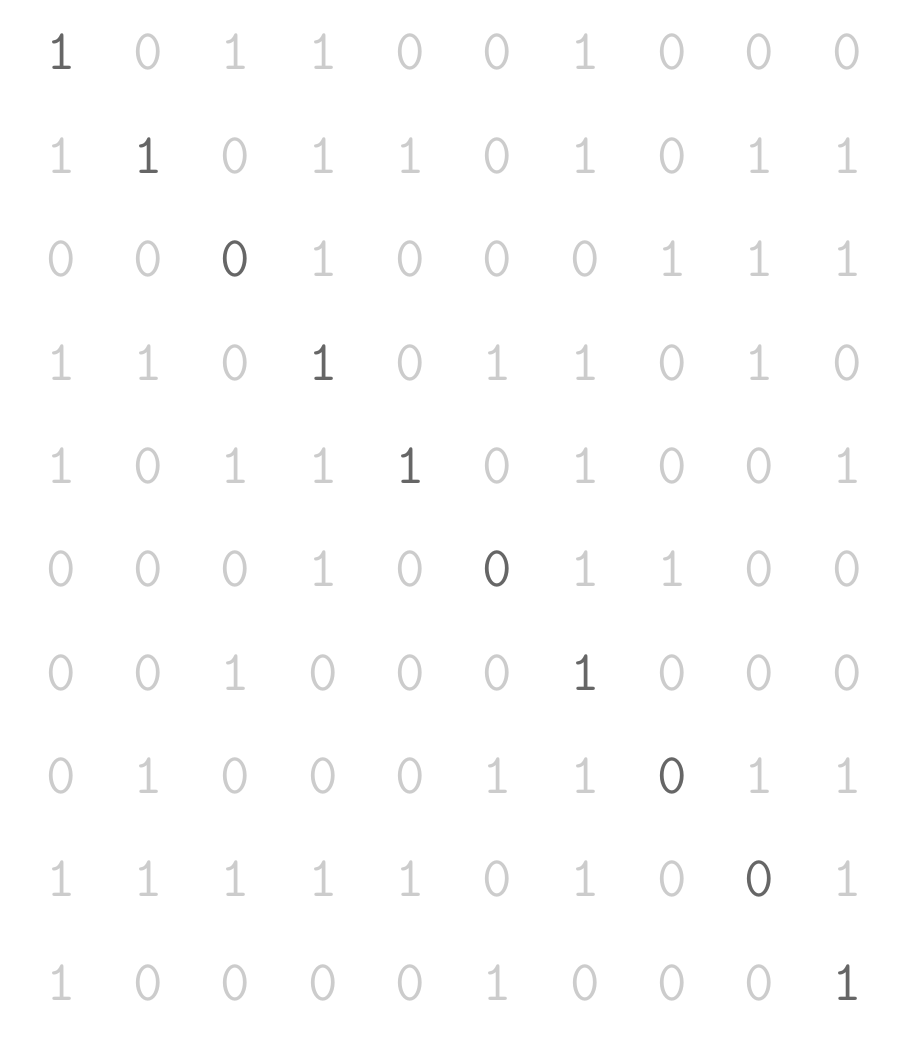
\begin{tikzpicture}[
				space/.style={minimum height=1.5em,matrix of nodes,row sep=7mm,column sep=5mm,style={font=\ttfamily}},text depth=0.5ex,text height=2ex,nodes in empty cells]
				\matrix (first) [space, style={font=\ttfamily}]
				{
				\odk & \zro & \one & \one & \zro & \zro & \one & \zro & \zro & \zro \\
				\one & \odk & \zro & \one & \one & \zro & \one & \zro & \one & \one \\
				\zro & \zro & \zdk & \one & \zro & \zro & \zro & \one & \one & \one \\
				\one & \one & \zro & \odk & \zro & \one & \one & \zro & \one & \zro \\
				\one & \zro & \one & \one & \odk & \zro & \one & \zro & \zro & \one \\
				\zro & \zro & \zro & \one & \zro & \zdk & \one & \one & \zro & \zro \\
				\zro & \zro & \one & \zro & \zro & \zro & \odk & \zro & \zro & \zro \\
				\zro & \one & \zro & \zro & \zro & \one & \one & \zdk & \one & \one \\
				\one & \one & \one & \one & \one & \zro & \one & \zro & \zdk & \one \\
				\one & \zro & \zro & \zro & \zro & \one & \zro & \zro & \zro & \odk \\
				};
				\end{tikzpicture}
				{\color{dark-gray} \noindent\rule{10.25cm}{2pt}}
				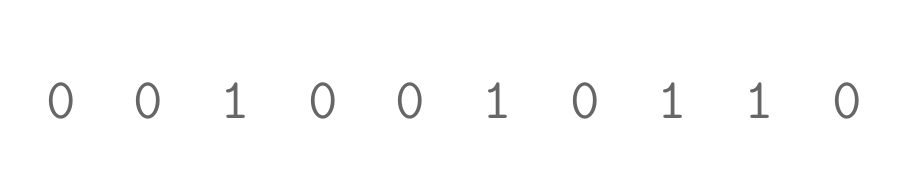
\begin{tikzpicture}[
				space/.style={minimum height=1.5em,matrix of nodes,row sep=0.1mm,column sep=5mm,style={font=\ttfamily}},text depth=0.5ex,text height=2ex,nodes in empty cells]
				\matrix (first) [space, style={font=\ttfamily}]
				{
					&&&&&&&&& \\
					\zdk & \zdk & \odk & \zdk & \zdk & \odk & \zdk & \odk & \odk & \zdk \\
				};
				\end{tikzpicture}
			\end{center}
		\end{tcolorbox}
		\vspace{1mm}
		{\fontsize{18}{20} \adforn{1}\hspace{8mm}\spacedlowsmallcaps{Tommy Monson}\hspace{8mm}\adforn{2}}
	\end{center}
\end{tcolorbox}
\end{titlepage}

\newpage

%--------------------------------------------------------------------------------
%--------------------------------------------------------------------------------
%    TABLE OF CONTENTS
%--------------------------------------------------------------------------------
%--------------------------------------------------------------------------------

\newgeometry{top=1.5cm,bottom=2.5cm,outer=4cm,inner=4cm}

\setcounter{tocdepth}{3} % Set the depth of the table of contents to show sections, subsections, and subsubsections

\tableofcontents % Print the table of contents

\newpage

%--------------------------------------------------------------------------------
%--------------------------------------------------------------------------------
%    PREFACE
%--------------------------------------------------------------------------------
%--------------------------------------------------------------------------------

\part*{Preface}
\addcontentsline{toc}{section}{Preface}

\begin{displayquote}
\textit{I wrote my first novel because I wanted to read it.}
\begin{flushright}
	---Toni Morrison
\end{flushright}
\vspace{4mm}
\end{displayquote}

% Why did you write this?
% Why do you think its worth sharing with others?
% College gave me reasoning and knowledge. Writing this guide gave me intuition.
% There are a lot of jargon terms in computer science, and a lot of them are very similar. This guide also serves as a personal dictionary of sorts.
% Wax poetic about computer science.

\newpage

%--------------------------------------------------------------------------------
%--------------------------------------------------------------------------------
%    A NOTE ON SOURCING
%--------------------------------------------------------------------------------
%--------------------------------------------------------------------------------

\part*{A Note on Sourcing}
\addcontentsline{toc}{section}{A Note on Sourcing}

\begin{displayquote}
	\textit{The origin of concepts, even for a scholar, is very difficult to trace. For a nonscholar such as me, it is easier. But less accurate.}
	\begin{flushright}
		---Peter Freyd
	\end{flushright}
	\vspace{4mm}
\end{displayquote}

% This guide was not written under the circumstances that a textbook would be. It is not intended to be a textbook.
% It was not written with sourcing in mind.
% However, all of the information here is the result of cross-referenced research.
% Philosophy of 98% accuracy.

\newpage

%--------------------------------------------------------------------------------
%--------------------------------------------------------------------------------
%    PART 0: INTRODUCTION
%--------------------------------------------------------------------------------
%--------------------------------------------------------------------------------

\part*{Introduction}
\addcontentsline{toc}{part}{\tocpartglyph Introduction}

This guide is everything you need to know in order to program computers professionally in the modern era.

% Redo this intro.
% Use short paragraphs. Be concise. Make it conversational.
% Make it inspiring. Make it motivational. Make sound accessible.
% Start with a philosophical idea of computation. Talk about how computation and calculation are human nature. Give broad overviews of the parts.
% Computation is a mechanical behavior. Let's build machines to do it for us.
% Certainty and objectivity are the pursuit of man. We pursue it via calculation and computation.
% Discuss the goal of this guide. Discuss why someone might want to read it.
% Discuss why content was chosen and why it is ordered the way it is.
% Discuss why certain topics were left out.
% Give a section by section overview. Raise some of the central questions.
% Give a warning for the Theory of Computation section lol. Or at least assure readers that things will become more applied as the guide progresses.
% Note differences in writing styles between the theory chapters (1-4) and the implementation chapters (5-7). The latter are not comprehensive overviews.
% Discuss the title. Information - data vs abstract concepts.

\newpage

%--------------------------------------------------------------------------------
%--------------------------------------------------------------------------------
%    PART I: THEORY OF COMPUTATION
%--------------------------------------------------------------------------------
%--------------------------------------------------------------------------------

\part*{Theory of Computation}
\addcontentsline{toc}{part}{\tocpartglyph Theory of Computation}

% Rewrite, be poetic about computation. Really describe it. Then discuss how the idea was generalized and formalized and found to have a lot of commonalities with language, logic, math...

The \textit{theory of computation} is a field of study that is related to both mathematics and computer science. It is concerned with a process known as \textit{computation}, which refers to any kind of \textit{calculation} (the transformation of one or more inputs into one or more outputs) that is accomplished by following an \textit{algorithm} (a set of rigorously defined steps). It is also concerned with the formalization of theoretical models of computation known as \textit{abstract machines} or \textit{abstract automata}. Also of interest are the \textit{computational problems} that can be solved by these abstract machines and how efficiently they can be solved. The theory of computation gives us the formal definition of a computer and the scope of what a computer can accomplish. \\

Much of the work in the theory of computation is$\dots$ quite abstract. While calculation and computation have been practiced by humans for thousands of years, the concept was only formalized by mathematicians, logicians, philosophers, linguists, and computer scientists in the past 150 years. This part of the guide will delve into some fairly academic topics with a decent amount of mathematical rigor, but it is written to be accessible and entertaining. \\

The field has three branches: \textit{automata theory}, \textit{computability theory}, and \textit{computational complexity theory}, each of which asks fundamental questions pertaining to how mathematical calculations can be automated, which kinds of problems can be solved by a machine, and how many resources are required to solve a particular problem. We will touch on the major discoveries made in each of these branches and discuss why they are significant to computer science and programming in general. \\

%--------------------------------------------------------------------------------
%    SECTION 1: AUTOMATA THEORY
%--------------------------------------------------------------------------------

\toclineskip
\section{Automata Theory}

% Concept of automata
% Models of computation
% Computation requires state, transition, and language

\textit{Automata theory} is the study of \textit{automata} and their behavior. An \textit{automaton} is a self-operating machine designed to follow or respond to a predetermined sequence of operations. Automata include physical devices such as cuckoo clocks, mechanical watches, robots, and computer processors as well as \textit{abstract machines}. An abstract machine is any formal description of \textit{mechanical behavior}. An abstract machine that is used to formally describe computation is called a \textit{model of computation}. This is a mathematical description of what a computer is, and it models the computation that a real, concrete computer could actually perform, if you were to implement that computer according to the model's specifications. Like their concrete counterparts, abstract machines have \textit{state}, a set of information in the \textit{present} that was acquired due to \textit{past} events. All automata begin with a \textit{starting state}, receive some sort of \textit{input}, and \textit{transition} to another state based on the value of that input and the value of its current state. \\

One \textit{abstract automaton} in particular fully models not only the computation that is performed by today's state-of-the-art computers, but also the very process of computation itself. We will spend a lot of time in this guide discussing the structure and behavior of this model as well as what its limitations imply regarding the future of computing, software, mathematics, and the meaning of life. We will also briefly explore the abstract automata that exist in pure mathematics and model computation that is not physically realizable. \\

%----------------------------------------

\subsection{States, Transitions, and Language}

% Creation of language, humanity stuff, natural language
% Alphabets, words, sentences, grammars
% Discuss language informally and formally
% Discuss grammar informally and formally

%----------------------------------------

\subsection{Exploring the Link Between Concrete and Abstract Machines}

Let's take a simple, concrete machine and try to visualize the abstract machine that underlies it. Consider a cuckoo clock. Every day, at noon, a small plank with a mechanical bird perched on its lip will extend from a hole above the clock face, powered by a working motor. Once the plank is fully extended, the bird will flap its metal wings and maybe turn its head as a song is played from a revolving music box inside the clock. Then, when it is 12:01 PM, the music will stop, the bird will still, and the plank will retract. The process will occur again the next day, at noon. \\

The machine's components here are the plank, the bird, and the music box. The components each have two states: the plank can be retracted or extended, the bird can be still or flapping its wings, and the music box can be paused or playing. The input to this machine is whether or not the clock hands both point straight at 12. We can say that this automaton has a state that can be expressed in terms of the states of its components. We can represent its starting state with the sequence (0,0,0) (i.e. the plank is retracted, the bird is still, and the music box is paused). The automaton can receive one of two inputs, 1 or 0 (i.e. both clock hands point straight at 12 or they do not). This input might be implemented with an electromechanical switch that turns the motor on or off.

\paragraph{(0,0,0) -> (1,0,0)} We start at state (0,0,0). As the morning passes, the automaton receives a constant input of 0, which keeps it in its starting state. At noon, the input switches to 1, and the automaton transitions to the state (1,0,0). As the plank extends and transitions its own state from 0 to 1, the bird remains still, and the music box remains paused. Once the plank is fully extended, we are in state (1,0,0).

\paragraph{(1,0,0) -> (1,1,1)} We expect that the plank will be fully extended well before 12:01 PM, so the input should still be 1. However, if for some reason the input is 0, we should transition back to (0,0,0), as the machine should only operate outside of its starting state between 12:00 and 12:01 PM. This is a simple example of \textit{strange input}. The input 0 at this state is unexpected, but it is technically possible. It is a better idea to define the behavior for this unexpected case, rather than to allow the input to cause unexpected behavior. On the other hand, if the input is 1 at this state, the automaton transitions to the state (1,1,1). The plank is fully extended, the bird is flapping its wings, and the music box is playing.

\paragraph{(1,1,1) -> (0,0,0)} Before 12:01 PM, the input is still 1, and that input should keep the automaton in its current state of (1,1,1). When 12:01 PM rolls around, the input will now be 0. In this case, we would like to return to the original state. On receipt of the input 0 while in state (1,1,1), the automaton transitions back to its starting state, (0,0,0). This abstract machine is shown below with a state format of (plank, bird, music) and an input specifying if the clock hands point exactly toward 12.

% Drawing of "Bad Automaton"
\begin{center}
	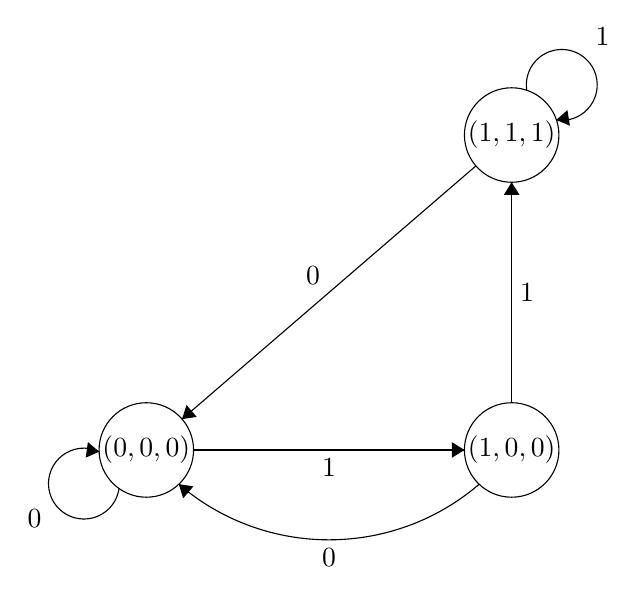
\begin{tikzpicture}[scale=0.2]
	\tikzstyle{every node}+=[inner sep=0pt]
	\draw [black] (28.4,-36.5) circle (3);
	\draw (28.4,-36.5) node {$(0,0,0)$};
	\draw [black] (51.6,-36.5) circle (3);
	\draw (51.6,-36.5) node {$(1,0,0)$};
	\draw [black] (51.6,-16.5) circle (3);
	\draw (51.6,-16.5) node {$(1,1,1)$};
	\draw [black] (31.4,-36.5) -- (48.6,-36.5);
	\fill [black] (48.6,-36.5) -- (47.8,-36) -- (47.8,-37);
	\draw (40,-37) node [below] {$1$};
	\draw [black] (51.6,-33.5) -- (51.6,-19.5);
	\fill [black] (51.6,-19.5) -- (51.1,-20.3) -- (52.1,-20.3);
	\draw (52.1,-26.5) node [right] {$1$};
	\draw [black] (26.668,-38.935) arc (-7.69924:-295.69924:2.25);
	\draw (21.78,-40.87) node [left] {$0$};
	\fill [black] (25.41,-36.61) -- (24.69,-36) -- (24.55,-36.99);
	\draw [black] (49.539,-38.673) arc (-49.35642:-130.64358:14.645);
	\fill [black] (30.46,-38.67) -- (30.74,-39.57) -- (31.39,-38.81);
	\draw (40,-42.71) node [below] {$0$};
	\draw [black] (52.56,-13.67) arc (189:-99:2.25);
	\draw (56.9,-10.25) node [right] {$1$};
	\fill [black] (54.43,-15.54) -- (55.3,-15.91) -- (55.14,-14.92);
	\draw [black] (49.33,-18.46) -- (30.67,-34.54);
	\fill [black] (30.67,-34.54) -- (31.6,-34.4) -- (30.95,-33.64);
	\draw (38.99,-26.01) node [above] {$0$};
	\end{tikzpicture}
\end{center}
\vspace{5mm}

This is a perfectly reasonable abstract machine, but something isn't right. It does not accurately simulate the behavior of the cuckoo clock we described. What happens when the clock strikes midnight? The clock hands will point at 12, producing an input of 1, but we don't want the bird to wake everyone up at midnight. We could use two bits of input: whether or not the hands are between 12:00 and 12:01, and whether it is AM or PM. Additionally, the music never plays unless the bird is flapping its wings, so we can combine those states. The abstract machine is better represented by the diagram below with a state format of (plank, bird/music) and an input format of (hands are toward 12, is PM).

% Drawing of "Good Automaton"
\begin{center}
	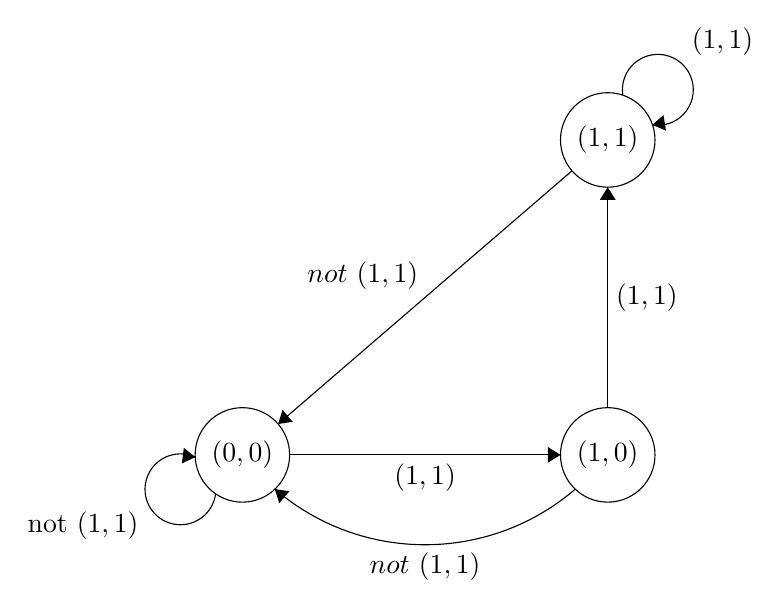
\begin{tikzpicture}[scale=0.2]
	\tikzstyle{every node}+=[inner sep=0pt]
	\draw [black] (28.4,-36.5) circle (3);
	\draw (28.4,-36.5) node {$(0,0)$};
	\draw [black] (51.6,-36.5) circle (3);
	\draw (51.6,-36.5) node {$(1,0)$};
	\draw [black] (51.6,-16.5) circle (3);
	\draw (51.6,-16.5) node {$(1,1)$};
	\draw [black] (31.4,-36.5) -- (48.6,-36.5);
	\fill [black] (48.6,-36.5) -- (47.8,-36) -- (47.8,-37);
	\draw (40,-37) node [below] {$(1,1)$};
	\draw [black] (51.6,-33.5) -- (51.6,-19.5);
	\fill [black] (51.6,-19.5) -- (51.1,-20.3) -- (52.1,-20.3);
	\draw (52.1,-26.5) node [right] {$(1,1)$};
	\draw [black] (26.699,-38.957) arc (-6.96472:-294.96472:2.25);
	\draw (21.83,-40.98) node [left] {not $(1,1)$};
	\fill [black] (25.42,-36.64) -- (24.68,-36.05) -- (24.56,-37.04);
	\draw [black] (49.539,-38.673) arc (-49.35642:-130.64358:14.645);
	\fill [black] (30.46,-38.67) -- (30.74,-39.57) -- (31.39,-38.81);
	\draw (40,-42.71) node [below] {$not\mbox{ }(1,1)$};
	\draw [black] (52.56,-13.67) arc (189:-99:2.25);
	\draw (56.9,-10.25) node [right] {$(1,1)$};
	\fill [black] (54.43,-15.54) -- (55.3,-15.91) -- (55.14,-14.92);
	\draw [black] (49.33,-18.46) -- (30.67,-34.54);
	\fill [black] (30.67,-34.54) -- (31.6,-34.4) -- (30.95,-33.64);
	\draw (36.05,-26.01) node [above] {$not\mbox{ }(1,1)$};
	\end{tikzpicture}
\end{center}
\vspace{5mm}

% Generalize this diagram to labelled transition system
% Transition system is a directed graph

% Transition system, semiautomaton, operator monoid
% F-coalgebra => transition systems are classes (math object)
% Difference between semiautomata and automata

Note that the actual complexity of the concrete cuckoo clock would be a bit more complicated than the automaton above. For example, what does the bird do specifically when it is on? Perhaps it raises and lowers its wings three times, turns its head to the right twice, and repeats. This process can be modeled by a different automaton. To fully model a concrete automaton, we must reduce it to an abstract machine, a system of states and transitions that account for every intended behavior. Abstract machines are capable of modeling systems of any arbitrary complexity. The automaton above is a model of computation called a \textit{finite-state machine} (FSM), and it will be the first abstract machine that we will discuss.
\\

% The nodes could themselves be automata => automata are recursive structures

%----------------------------------------

\subsection{Classes of Automata and the Languages They Can Understand}

Automata, in general, are machines that receive, interpret, and follow instructions that are written according to the \textit{grammar} of a \textit{formal language}. Formal languages are similar to the \textit{natural languages} that humans speak in that they have \textit{words} that conform to a \textit{syntax} that is specified in terms of symbols from an \textit{alphabet}. These words can be arranged according to a \textit{grammar} to form \textit{sentences}, from which \textit{semantic meaning} can be interpreted. However, unlike natural languages, they are defined in precise, unambiguous terms. \\

A formal language $L$ over an \textit{alphabet} $\Sigma$ is a \textit{set of words} that is a subset of $\Sigma^*$, the set of \textit{all} possible words that can be composed using $\Sigma$. Typically, formal languages conform to a \textit{formal grammar}, which is a set of precise grammatical rules. However, not all formal grammars are equal. Grammars determine how words can be arranged into sentences, which determines the kinds of thoughts that can be expressed. Thus, grammar controls how \textit{powerful} or \textit{expressive} a language is. If we intend to use a particular formal language to instruct a computer to solve a problem, the \textit{expressiveness} of the language will determine the kinds of instructions we are able to give. If we cannot express a given instruction, we will not be able to solve any problems requiring that instruction. \\

In this section, we will examine automata with different \textit{mechanical structures}. The \textit{data} that are stored in components of these structures can be interpreted as words, and the structures themselves can be used to represent the rules of a formal grammar. However, some expressive grammars cannot be represented by simpler structures. Thus, the mechanical structure of an automaton acts as an \textit{upper bound} on its \textit{capacity} to understand language, and, by extension, its computational versatility. \\\\

\begin{tcolorbox}[breakable, enhanced, colback=textbook-blue, sharp corners]
	\vspace{2mm}
	\begin{center}
		\textbf{A Brief Introduction to Formal Grammars}
	\end{center}
	\vspace{1mm}
	A formal grammar is a finite set of \textit{production rules} that specifies what a particular language is supposed to look like. It formalizes the structure of "grammatical units" in a language. This is done in order to enforce a specific alphabet, a consistent lexicon, and a predictable sentence structure, all of which contribute to how useful and distinct any given language is. \\
	
	A grammar $G$ consists of the following components:
	\begin{itemize}
		\item A finite set $N$ of \textit{nonterminal} symbols.
		\item A finite set $\Sigma$ of \textit{terminal} symbols that is disjoint from $N$.
		\item A symbol $S\in N$, designated as the \textit{start symbol}.
		\item A finite set $P$ of \textit{production rules} where each rule is of the form ${(\Sigma\cup N)^*N(\Sigma\cup N)^*\rightarrow(\Sigma\cup N)^*}$.
	\end{itemize}

	Put another way, a production rule converts a sequence of symbols to another sequence of symbols. If a rule is of the form \textit{left-hand side $\rightarrow$ right-hand side}, each side can contain terminals and nonterminals, but its left-hand side must contain at least one nonterminal. A nonterminal is a symbol that is replaced by other symbols when an appropriate rule is applied. Unlike a terminal, it does not belong to the alphabet of the language, but rather represents a sequence of symbols that do. Terminals cannot be replaced by other symbols once chosen. \\
	
	Let's construct a simple formal grammar. It is typical for the nonterminals to be uppercase and for the terminals to be lowercase. Let $N=$ \{SENTENCE, NOUN, ADJ\}, $\Sigma=$ \{the, dog, building, plays, fluffy, good\}, and $S=$ SENTENCE. The rules of $P$ are given below.
	
	\begin{itemize}
		\item SENTENCE $\rightarrow$ the NOUN plays
		\item NOUN $\rightarrow$ ADJ NOUN
		\item NOUN $\rightarrow$ dog
		\item NOUN $\rightarrow$ building
		\item ADJ $\rightarrow$ fluffy
		\item ADJ $\rightarrow$ good
	\end{itemize}
	
	We can now start with SENTENCE and apply these rules to construct a "sentence" that is valid in this language. Example sentences and their derivations are given below.
	
	\begin{itemize}
		\item SENTENCE $\rightarrow$ the NOUN plays $\rightarrow$ the ADJ NOUN plays $\rightarrow$ the good NOUN plays $\rightarrow$ the good dog plays
		\item SENTENCE $\rightarrow$ the NOUN plays $\rightarrow$ the ADJ NOUN plays $\rightarrow$ the ADJ ADJ NOUN plays $\rightarrow$ the ADJ ADJ ADJ NOUN plays $\rightarrow$ the fluffy ADJ ADJ NOUN plays $\rightarrow$ the fluffy good ADJ NOUN plays $\rightarrow$ the fluffy good fluffy NOUN plays $\rightarrow$ the fluffy good fluffy building plays
	\end{itemize}

	Notice that the first example expresses an actual thought whereas the second example, while still syntactically a sentence, is nonsensical. Because it allows meaningless sentences, the grammar described above belongs to the class of \textit{context-free grammars}.
	
	\vspace{1mm}
\end{tcolorbox}
\vspace{7mm}

Before we discuss and classify automata in depth, we should first consider what is \textbf{not} an automaton. What is an example of something that might perform some kind of calculation, but is not a computer? What about a microwave? Is a microwave a computer? No, it is not. A computer can be programmed in some meaningful, robust way. A microwave contains a microprocessor, which uses \textit{combinational logic} and basic binary inputs to set timers and operate the oven. It cannot be programmed in any meaningful way. What about a calculator? Is a calculator a computer? If we are being formal, the answer is no, but it depends on what kind of "calculator" we are talking about. \\

Calculators, such as \textit{counting boards} and the \textit{abacus}, have been around since pre-history. Calculators with four-function capabilities have been around since the invention of Wilhelm Schickard's mechanical calculator in 1642. In the late 19th century, the \textit{arithmometer} and comptometers, two kinds of digital, mechanical calculator, were being used in offices. The Dalton Adding Machine introduced buttons to the calculator in 1902, and pocket mechanical calculators became widespread in 1948 with the \textit{Curta}. None of these are computers. \\

The difference between a calculator and a computer is that a computer can be programmed and a calculator cannot. What does it mean to be programmable? That is perhaps the central question of automata theory, and we will discuss in this section several levels of "programmability". However, for now, we can certainly say that a simple, four-function electronic calculator is not a computer. It simply uses combinational circuits like full-adders, full-subtractors, multipliers, and dividers to implement its functions, and there is no potential for modifications or user-defined functions. \\

Surprisingly enough, \textit{special-purpose computers} have also been around for a long time. Early examples include the \textit{Antikythera mechanism} (an Ancient Greek analog computer), Al-Jazari's 1206 water-powered \textit{astronomical clock}, the 1774 \hrefcolor[blue]{https://www.youtube.com/watch?v=bY\_wfKVjuJM}{\underline{Writer Automaton}} (a mechanical doll that could be programmed to write messages), the 1801 \textit{Jacquard loom}, and \textit{slide rules}. Some later mechanical computers were quite powerful, such as \textit{differential analyzers} (special-purpose computers for solving differential equations) and \hrefcolor[blue]{https://www.youtube.com/watch?v=s1i-dnAH9Y4}{\underline{fire control computers}}. Charles Babbage designed the \textit{Analytical Engine}, a general-purpose computer, in 1837, and Ada Lovelace wrote a program for it, but it was never built. General-purpose computing would not reemerge until the 1940s. \\

The line between calculator and computer began to blur with the introduction of \textit{programmable calculators} in the 1960s. Many modern high-end calculators are programmable in Turing-complete languages such as TI-BASIC or even C or C++, which officially makes them computers. Once we start implementing \textit{sequential logic} with components like SR latches or D flip-flops, we are storing state, and state is a requirement for computing. Circuits that use sequential logic can be considered automata and, given enough complexity, computers. \\

We will now discuss four classes of automata, in increasing order of complexity. As they become more complex, automata are able to recognize more powerful and expressive languages. They can be told to execute \textit{instructions} in these languages, and they will be able to accomplish more complex tasks if their language is more expressive. When we reach the last of these four automata, we will be talking about the most powerful model of computation that is feasible to build, the automaton that models modern general-purpose computers. Once we explore this particularly important automaton in depth, we will learn how it can be modified to model more exotic forms of computation. \\

\subsubsection{Finite-state Machines}

A finite-state machine is a model of computation that can be in exactly one \textit{state} from a finite set of states at any given time. Given its current state and an input, an FSM can \textit{transition} to another state. \textit{Deterministic finite automata} (DFA) are FSMs that transition to at most one state for each input. In contrast, \textit{nondeterministic finite automata} (NFA) can transition to zero or more states for each input. It follows then that a DFA is a special kind of NFA. An FSM may also have a subset of states that are considered \textit{final states}. When the machine transitions to one of these states, it will finish its work and cease operation. \\

FSMs can read and understand \textit{regular languages}, which are languages that can be expressed using a \textit{regular expression} or \textit{regex}. A regex consists of constants (which denote sets of strings) and operators (which denote operations on those sets). If an FSM receives an input (such as a regex) at a given state, and its state-transition function maps that state and input to another state, we say that the FSM \textit{matches} that input. That is, it considers that input valid and will perform an action accordingly. \\\\

\begin{tcolorbox}[breakable, enhanced, colback=textbook-blue, sharp corners]
	\vspace{2mm}
	\begin{center}
		\textbf{A Quick Summary of Regular Expressions}
	\end{center}
	\vspace{1mm}

	Given a finite, non-empty input alphabet $\Sigma$, there are three constants defined as regexes:
	
	\begin{itemize}
		\item The \textit{empty set}, $\emptyset$, which denotes the set containing no elements.
		\item The \textit{empty string}, $\varepsilon$, which denotes the set containing only the empty string "".
		\item A \textit{literal character} (e.g. the character $a$ denotes the set containing only the character "$a$").
	\end{itemize}
	
	These constants can be combined and manipulated with operators to create long, complex regular expressions. There are three operators that operate on regexes, which are described below in increasing order of priority. Given regular expressions $A$ and $B$, the operations include:
	
	\begin{itemize}
		\item The \textit{concatenation} of $A$ and $B$, $AB$, which denotes the set of strings that can be created by concatenating a string in $A$ with a string in $B$.
		\item The \textit{alternation} of $A$ and $B$, $A|B$, which denotes the union set of $A$ and $B$.
		\item The \textit{Kleene star} of $A$, $A^*$, which denotes the set of all strings that can be created by concatenating a finite number of strings (including zero strings) from the set $A$.
	\end{itemize}
	
	Two additional operators are added as "syntactic sugar": $+$ and $?$. Whereas the literal character $a$ denotes the set of strings that contain a single $a$ and nothing else, the regex $a+$ denotes the set of strings that contain \textit{at least one} $a$ and nothing else and the regex $a?$ denotes the set of strings that contain \textit{at most one} $a$ and nothing else. Thus, $a+=aa^*$ and $a?=a|\varepsilon$. \\
	
	A variety of \textit{metacharacters} are also often used in order to create more concise regexes. Common metacharacters include:
	
	\begin{itemize}
		\item $\hat{}\;$, which matches the starting position in a line of text.
		\item $\$$, which matches the ending position in a line of text.
		\item $.$, the \textit{wildcard}, which matches any character.
		\item $-$, which, when placed between two regexes in brackets, denotes a range of characters.
		\item $[\;\hat{}\quad]$, which matches a single character which is not in the brackets.
	\end{itemize}
	\vspace{1mm}
\end{tcolorbox}
\vspace{7mm}

Not only is it correct to say that a finite-state machine can understand any regular expression, but also it is true that FSMs and regexes are equivalent. That is, a regex can be written in the form of an FSM and vice versa. Indeed, a regular language "program" can be expressed as a regex, a DFA, or an NFA. For example, the regex [A-Z][a-z]$^*$[0-9] describes any string that starts with a single uppercase letter, is followed by zero or more lowercase letters, and ends with a single digit. This expression can also be represented by the following DFA. Note that state $3$ is circled twice to indicate that it is a final state. The automaton will continue to run until it receives a sequence of input that allows it to transition to its final state.\\

\vspace{3mm}
\begin{center}
	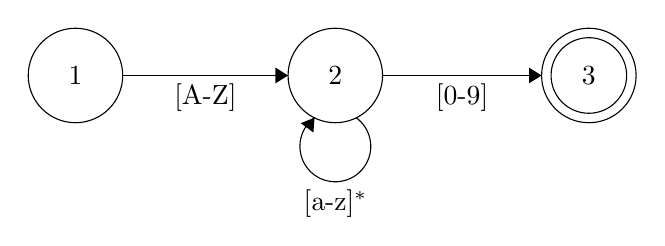
\begin{tikzpicture}[scale=0.2]
	\tikzstyle{every node}+=[inner sep=0pt]
	\draw [black] (22.9,-27) circle (3);
	\draw (22.9,-27) node {$1$};
	\draw [black] (39.4,-27) circle (3);
	\draw (39.4,-27) node {$2$};
	\draw [black] (55.5,-27) circle (3);
	\draw (55.5,-27) node {$3$};
	\draw [black] (55.5,-27) circle (2.4);
	\draw [black] (25.9,-27) -- (36.4,-27);
	\fill [black] (36.4,-27) -- (35.6,-26.5) -- (35.6,-27.5);
	\draw (31.15,-27.5) node [below] {[A-Z]};
	\draw [black] (42.4,-27) -- (52.5,-27);
	\fill [black] (52.5,-27) -- (51.7,-26.5) -- (51.7,-27.5);
	\draw (47.45,-27.5) node [below] {[0-9]};
	\draw [black] (40.723,-29.68) arc (54:-234:2.25);
	\draw (39.4,-34.25) node [below] {[a-z]$^*$};
	\fill [black] (38.08,-29.68) -- (37.2,-30.03) -- (38.01,-30.62);
	\end{tikzpicture}
\end{center}
\vspace{5mm}

Regular languages and, by extension, finite-state machines are often used in string searching algorithms. FSMs and regular languages are also often used in the lexical analysis (lexing) done by a compiler. That is, they give language designers the power to specify which words are valid in their programming language. \\

\subsubsection{Pushdown Automata}

Pushdown automata (PDA) are finite-state machines that also have access to a stack. These automata introduce a notion of \textit{history} or \textit{memory}. A PDA can push a symbol onto its stack on every transition, which will provide information in the future about actions in the past. It can also pop or peek at the stack to decide which transition to take next. \\

Pushdown automata can distinguish syntactically correct sentences from random sequences of valid words, something finite-state automata cannot do because they have no notion of what comes earlier than a given point in a given sentence. For example, a pushdown automaton would be able to tell that "my dog bites red toys" is a valid English sentence and "red my toys dog bites" is not. However, PDA cannot understand semantics. It would also consider "my dog \textit{barks} red toys" a valid English sentence, even though it has no meaning. \\

Pushdown automata can read \textit{context-free languages}, which are languages that follow a \textit{context-free grammar}. Context-free languages are formal languages whose production rules are of the form $A\rightarrow\alpha$ where $A$ is a nonterminal and $\alpha$ is a sequence that may contain terminals and nonterminals. A PDA pops terminals from its stack. When a nonterminal $A$ is at the top of the stack, the PDA can pop it and push the $\alpha$ of some production rule onto the stack. In a sense, the stack of the PDA contains the unprocessed data of the grammar. \\

Context-free grammars can be written to formalize languages such as the language of matching parentheses or the language of infix algebraic expressions (e.g. (2+4)/7*8). PDA and context-free languages are often used in the syntactic analysis (parsing) done by a compiler. That is, they give language designers the power to specify how valid sentences are structured in their programming language. \\

\subsubsection{Linear Bounded Automata}

Imagine that, instead of a stack, an automaton could have access to a finite-length list. Linear bounded automata (LBA) have a finite number of \textit{states}, a finite length of \textit{tape}, and a \textit{head} that can read and write symbols on the tape and move left or right along it, one symbol at a time. The length of the tape is a linear function of the length of the input, so we can say that the tape has $kn$ cells, where $n$ is the length of the input instructions and $k$ is a constant. \\

This machine is similar to the idea of a modern computer. The tape represents a finite amount of memory, and the head is able to read and write to it. LBA can understand \textit{context-sensitive languages}, which are languages that follow a \textit{context-sensitive grammar}. Sophisticated programming languages are context-sensitive, so a linear bounded automaton would be able to read and understand modern software. The $kn$-length tape acts as a sufficient environment for computationally demanding programming tasks, given a large enough $k$. Similarly, given enough memory, real computers can also solve very computationally difficult problems. \\

A context-sensitive language is a language where semantics matter. Using our earlier example, "my dog barks red toys" would not be a valid sentence in a context-sensitive version of English. An LBA then is actually able to differentiate data types and can tell when an operation is defined for one type and undefined for another. LBA and context-sensitive languages are often used in the semantic analysis (type checking) done by a compiler. That is, they give language designers the power to specify whether or not a syntactically correct sentence actually has any real \textit{meaning} in their programming language. \\

Where can we go from here? LBA are suitable models of real-world computers, and they can process semantic language. What more can we do? Let's try making the tape infinitely long$\dots$ \\

\subsubsection{Turing Machines}

A \textit{Turing machine} (TM) not only models real-world computers, but \textit{computation} itself. The concept, which was formalized in 1936 by Alan Turing, generalizes automata and defines the limitations of mechanical computing. It specifies a set of components that are necessary and sufficient for creating a "problem-solving machine" that is capable of solving any problem that can be solved by a machine. Weaker automata can solve \textit{some} of these machine-solvable problems, but only \textit{Turing-complete} automata (those that are functionally equivalent to TMs) have the expressive power to solve \textit{any} of them. The components of a Turing machine are listed below.

\begin{itemize}
\item An infinitely long \textit{tape} that is divided into cells, each of which contains a symbol from some finite alphabet. One symbol from this alphabet is considered blank, and the tape is initially filled with these symbols.
\item A \textit{head} that can read and write symbols on the tape and move left or right along it, one symbol at a time.
\item A \textit{state register} that stores its current state and initially stores its starting state.
\item A \textit{finite table of instructions} that, given the machine's current state and tape symbol, tells the machine to do the following sequence of actions:
	\begin{enumerate}
		\item Erase or write a symbol at the current tape cell (or do nothing)
		\item Move the head one tape cell to the left or right (or do nothing).
		\item Depending on the current state and input, transition to a different state (or the same state) or halt computation.
	\end{enumerate}
\end{itemize}

A machine like this need not be a real-world computer. In fact, in his original proof, \textit{On Computable Numbers, with an Application to the Entscheidungsproblem}, Turing refers to a person, whom he calls the "computer", as an example of a Turing machine. If we break down these components into the resources they represent, it becomes clear that many systems could be considered Turing machines.

\begin{itemize}
	\item The infinitely long tape represents \textit{infinite space for computation} or \textit{infinite memory}.
	\item The head represents three abilities:
		\begin{enumerate}
			\item Reading memory,
			\item Writing to memory,
			\item Traversing the memory freely, with no side effects.
		\end{enumerate}
	\item The state register represents the ability to \textit{know what "step" you are on} in the problem-solving process. We will clarify this ambiguous idea in a second, but for now just think of it as having an idea of your progress.
	\item The finite table of instructions represents a \textit{sequence of commands} or \textit{program} that can be followed unambiguously. The automaton can follow and obey these commands in order without any actual thought.
\end{itemize}

As long as you have unlimited space to work in, the freedom to read and write symbols anywhere in that space, a list of instructions to follow exactly, and the knowledge of what to do next, you have a Turing machine. We can now visualize the person Turing referred to as a "computer". It is a man with an infinitely large piece of paper, a pen that he writes symbols with, a list of instructions that tells him which symbols to write, where on the paper to move his pen tip, which instruction to perform next, and a knowledge of which instruction he is currently performing. Many systems of logic, such as programming languages, are Turing-complete. Many things not traditionally thought of as "systems of logic" are \hrefcolor[blue]{https://www.toothycat.net/~hologram/Turing/index.html}{\underline{also Turing-complete}}. \\\\

\begin{tcolorbox}[breakable, enhanced, colback=textbook-blue, sharp corners]
	\vspace{2mm}
	\begin{center}
		\textbf{Turing Machines and Consciousness}
	\end{center}
	\vspace{1mm}
	In 1950, Turing developed the \textit{Turing test}, a test of a machine's ability to exhibit behavior indistinguishable from that of a human. It involves an interrogator who is tasked with having two separate text conversations and determining which of the two participants is actually a machine. If the interrogator cannot distinguish a difference, the machine has passed the test. Despite its importance to the philosophy of computer science, the test is not a good indicator of whether or not a computer can think. The test says more about how gullible the interrogator is than how conscious the computer is. At the end of the day, the computer is still following its programming. \\
	
	What about this man whom Turing calls a "computer"? Would he pass the test, given the right programming? Perhaps he would. But that would not make him a \textit{person}. What kind of person is this man if he follows whatever instructions he is given? He is a slave, a person who always obeys. Could we say then that machines are also, in a certain sense of the word, slaves? Perhaps this is where the term \textit{master-slave technology} came from. Regardless, it is important to make a philosophical distinction here about what separates humans from machines or, more precisely, what distinguishes \textit{thought} from \textit{computation}. \\
	
	Essentially, this boils down to the question of consciousness. There is much debate about consciousness. Philosophers have proposed a variety of concepts that partially define it such as free will (the ability to choose) or qualia (the raw experience of existence, e.g. sounds, colors, emotions). However, \textit{intentionality} is one characteristic that is generally agreed upon as necessary for conscious thought. Intentionality is the ability of the mind to think \textit{about} something. Computers can \textit{think} things, but they cannot \textit{think about} things. They lack intentionality.\\
	
	For a Turing machine, the list of instructions is an essential component. It is capable of "thinking" if and only if some one tells it what to think. That effort is more accurately defined by the term "computation". We would also refer to the man's efforts with his pen and infinite paper as computations because they require no thought. If he were nothing more than a Turing machine, the man would not be able to perform mathematics on his own. In fact, he would not be able to do anything without instructions. It is the moment when he does something without being explicitly told to do it that he first displays consciousness. When \textit{unprompted} computation is performed for some \textit{purpose}, we can talk about consciousness. \\
	
	So calling computers slaves is a bit of an anthropomorphization. A slave is a conscious being who is forced to act like a machine. Computers don't have the prerequisite consciousness. No matter how complicated its architecture or sophisticated its artificial intelligence software, a computer is a \textit{tool} like a microwave or a calculator. Could it ever be more than that? Could a technology ever think? \hrefcolor[blue]{https://en.wikipedia.org/wiki/Artificial\_consciousness}{\underline{Perhaps}}. But such a thing would be quite different from a Turing machine or any modern computer. \\
	
	\parbreak
	\vspace{1mm}
	
	\begin{displayquote}
		\textit{In attempting to construct such machines we should not be irreverently usurping His power of creating souls, any more than we are in the procreation of children: rather we are, in either case, instruments of His will providing mansions for the souls that He creates.}
		\vspace{4mm}
		\begin{flushright}
			---Alan Turing (1950), \\
			in response to a theological objection to artificial consciousness.
		\end{flushright}
	\end{displayquote}
	\vspace{1mm}
\end{tcolorbox}
\vspace{7mm}

A single-tape Turing machine is formally defined as a septuple $(Q,\Gamma,b,\Sigma,\delta,q_0,F)$, where

\begin{itemize}
	\item $Q$ is a finite, non-empty set of \textit{states},
	\item $\Gamma$ is a finite, non-empty \textit{tape alphabet},
	\item $b\in\Gamma$ is the \textit{blank symbol},
	\item $\Sigma\subseteq\Gamma\setminus \{b\}$ is the set of symbols that can be written on the tape,
	\item $\delta$ is a partial function $\delta : (Q\setminus F)\times\Gamma\nrightarrow \Gamma\times\{L,R\}\times Q$ called the \textit{transition function}, which inputs the current state and tape symbol and outputs the symbol to write to the tape, the direction to move the head, and the next state to transition to,
	\item $q_0\in Q$ is the \textit{starting state}, and
	\item $F\subseteq Q$ is the set of \textit{final states}. The contents of the tape are \textit{accepted} if the Turing machine halts computation in a state from $F$.
\end{itemize}

We should now address what exactly "state" is in regard to computing. Many people associate it with the current instruction being fed to the machine. However, Turing made a distinction between this interpretation of state and the interpretation of state as the computer's "progress" or "state of mind". Turing's \textit{complete configuration} of state includes not only the current instruction, but the current symbol configuration of the entire tape as well and all the instructions yet to be executed. In this way, state is defined by the results of past instructions and the inevitable execution of future instructions. \\

Now we have defined what a Turing machine is, but it is still not clear why it is considered such a landmark concept in computer science. For example, if real-world computers can be sufficiently modeled by linear bounded automata, why do we instead focus so heavily on Turing machines? \\

Turing machines are the class of automata that can read \textit{recursively enumerable languages}. A formal language is called recursively enumerable, if it is a \textit{recursively enumerable subset} in the set of all possible words over the alphabet of the language. This essentially means that, for a language of this type, there exists an algorithm that can output a list of every word in the language. Consider what would be required for such an algorithm. How many valid words are there in a given language? Depending on its rules for constructing words, there may be an infinite amount. This is the case for some programming languages. A variable name could theoretically be as long as you want, provided you have enough memory to store it. In order to list all of the words in a recursively enumerable language, you would need infinite memory, which only a Turing machine can provide. \\

This does not imply that TMs can handle infinite lists of instructions. Rather, they can handle \textit{infinite looping} over a finite set of instructions. A Turing machine can "successfully" run a never-ending program. A real machine would use up all of its memory trying to run such a program, eventually crashing due to a \textit{stack overflow} (an attempt to write data outside of the limits of the memory). A TM would never run out of memory and, given infinite time, could run the program forever. \\

As previously stated, the Turing machine models not only computers, but \textit{computation}. It abstracts away the physical limitations of computers such as memory constraints, overheating, or hardware failure and asks what the fundamental limits of algorithmic computation are. It makes a statement on which mathematical problems are \textit{decidable}. It is an ideal computer, and, as such, it is not only a model of what real-world computers are today, but a model of what they \textit{could be} in the future, given sufficient advances in hardware. \\

%----------------------------------------

\subsection{The Importance of Turing Machines to Modern Computing}

The automata we have discussed so far (finite-state machines, pushdown automata, linear bounded automata, and Turing machines) form a sort of hierarchy of machine capability. The formal grammars and languages that these automata can understand likewise constitute a hierarchy that was first described by Noam Chomsky in 1956. The \textit{Chomsky hierarchy}, a classification of the expressiveness of language according to grammatical rules, is summarized below by a table with columns for grammars, the languages those grammars build, and the class of automaton that can understand those languages.

\begin{table}[H]
	\caption{The Chomsky Hierarchy}
	\label{tab:LABEL}
	\begin{tabularx}{\textwidth}{|c|c|Y|}
		\vtabularspace{3}
		\hline
		Grammar & Language & Automaton \\
		\hline
		Type-0 & Recursively enumerable & Turing machine \\
		Type-1 & Context-sensitive & Linear bounded automaton \\
		Type-2 & Context-free & Pushdown automaton \\
		Type-3 & Regular & Finite-state machine \\
		\hline
		\vtabularspace{3}
	\end{tabularx}
\end{table}

As this is a hierarchy, higher-ranking automata are capable of doing anything that lower-ranking automata can. For example, an LBA can do anything that a PDA or FSM can and \textit{more}. To give a linguistic analogy, an LBA would be fluent in all of the languages that the PDA and FSM are fluent in, but would also be fluent in additional languages. What causes this difference in language facility? It is the structure of the automaton's memory. \\

Let's recap how these four automata handle memory.

\begin{itemize}
	\item An FSM has \textit{no} memory. It simply has a finite number of states, perhaps represented by a finite list of instructions. It can transition between states, but it has no notion of how it got to any particular state. It records no history.
	\item A PDA has a \textit{stack} of memory, but this form of memory is restricted. It cannot read or write its memory in any order it likes. It can read the top entry on the stack, but it must delete data to read entries located elsewhere.
	\item An LBA has a \textit{finite array} of memory. It can read or write this memory in any order it likes, but it has limitations on how much information it can store.
	\item A TM has an \textit{infinite array} of memory. It can read or write this memory in any order it likes, and it can also store as much as it likes.
\end{itemize}

It is no coincidence that real-world computers today use array-based memory. Arrays are both an intuitive and Turing-complete way to store information. Now, technically, LBA and TMs use "tape" instead of arrays, but the differences are minimal. In tape memory, cells have relative position, but they are not \textit{labeled}. Modern computers are actually modeled by \textit{register machines}. Register machines are equivalent in expressive power to Turing machines, but their memory is composed of an infinite-length array of uniquely addressed \textit{registers}. Like a tape of cells, an array of registers can be freely accessed. \\

A subset of register machines known as \textit{random-access machines} allow for \textsc{jump} instructions (e.g. jump to register \#5623) in addition to standard sequential traversal of memory (e.g. move right, move right, move right, etc). This allows computers to accomplish a task with fewer instructions, but the expressive powers of random-access machines and Turing machines are equivalent because both are capable of \textit{eventually} solving the task. Modern computers can be described as random-access machines because they use \textit{random-access memory} (RAM). In RAM, the time to access information is independent of physical location. From a performance perspective, this means that we do not have to consider \textit{where} we store things in memory. It's all uniformly fast. This allows for the construction of \textit{node-based} data structures, which we will discuss in a later section. \\\\

\begin{tcolorbox}[breakable, enhanced, colback=textbook-blue, sharp corners]
	\vspace{2mm}
	\begin{center}
		\textbf{Exploring Exotic Automata}
	\end{center}
	\vspace{1mm}
	It is worth thinking about automata whose memory is modeled by non-list data structures. For example, a pushdown automaton uses a stack to model its memory and because of this, it is not Turing-complete. What if it used a queue instead? In this case, it would be Turing-complete because it could dequeue items to traverse the memory and then enqueue them to avoid data loss. One could envision this as a Turing machine whose infinite tape ends are glued together to form an infinite loop. The machine can only move in one direction, but it can still access every cell because its tape is circular. \\
	
	The memory can also be modeled by non-sequential data structures to create some bizarre models of computation. What if the memory of a computer was laid out not as an array, but as an undirected tree? What if it was organized according to an algebraic structure like a monoid or a ring? I'm not even going to pretend that I understand what kind of behavior this would result in. But it is an \hrefcolor[blue]{https://kluedo.ub.uni-kl.de/frontdoor/index/index/docId/4400}{\underline{area of active research}}. \\
	
	Other tweaks can be made to the properties of a Turing machine to create new, interesting automata. For example, \textit{$\omega$-automata} (or \textit{stream automata}) are Turing machines that expect an \textit{infinite} sequence of instructions. \textit{$\omega$-automata} never stop running because an infinite sequence of instructions requires an infinite sequence of instruction executions. Because they never terminate, they never move into acceptance (final) states. Rather than a set of final states $F$, they have a set of \textit{acceptance conditions} $Acc$. \\
	
	For ordinary automata, every \textit{run} $\rho$ (i.e. a sequence of $n$ states) ends with a state $r_n$, and the input is only accepted if this state is final (i.e. $r_n\in F$). For $\omega$-automata, runs are infinite sequences, so they do not end with a state $r_n$ at all. How do we tell if a run $\rho$ should be accepted as a valid set of instructions? We require that $\rho\in Acc$. That is, if the run is a member of the "set of acceptable runs", it should be accepted. What is the "set of acceptable runs"? That depends on which variant of $\omega$-automaton you are talking about. \\
	
	The class of $\omega$-automata contains multiple automata with different definitions of $Acc$. For example, for some subset $F$ (final states) of $Q$ (all states), the \textit{B\"{u}chi automaton} accepts those runs $\rho$, for which there exists a final state that occurs "infinitely often" in $\rho$. What is a state that is visited "infinitely often"? Given an infinite amount of runtime, some states in $Q$ will be visited an infinite amount of times, and others will not. For example, what if you can transition away from your starting state $q_0$, but you are not allowed to transition into it. Even given infinite time, $q_0$ would not be visited infinitely often, and if it were the only state in $F$, you would never be able to construct a run that would be considered valid by a B\"{u}chi automaton. Nondeterministic B\"{u}chi automata have applications in "always-on" or "always listening" software, such as those used in highly-autonomous robots or smart speakers like the Amazon Echo, both of which receive instructions based on a never-ending, real-time stream of sensory data. \\
	
	Wow, that's a lot of abstract mathematics. Why is any of this important for gaining a fundamental understanding of Turing machines or real-world computers? It is important because we can only really grasp their \textit{scope} if we explore outside of it. Some automata can have properties that are not practical or possible to implement in the real-world. Mathematically, they could have infinite states or continuous alphabets or hyperdimensional memory. But here, once and for all, let's define the scope of computation we will be considering for the rest of this guide. \\
	
	A modern computer has:
	
	\begin{itemize}
		\item A \textbf{finite} set of states Q. If it were instead infinite, the automaton would have a state for every possible input, and thus would be able to understand any conceivable language. This is far too powerful a machine to build. This would essentially be a universal problem solver.
		\item A \textbf{finite} alphabet $\Sigma$. If it were instead infinite, the automaton could have a continuous alphabet. What kind of alphabet's symbols exist on a spectrum? Perhaps you could call \textit{sound} a "language" with a continuous alphabet known as frequency. An automaton with an infinite alphabet would not be digital and would not use bits. It would be an analog computer. Analog computers do exist, and they were popular in the 1950s and 1960s, but nowadays we write software for digital computers. \textit{Fun fact:} analog synthesizers, which are still commonly used in electronic music, are considered a kind of analog computer.
		\item A transition \textbf{function} $\delta$. If it were instead a relation (i.e. inputs are mapped to more than one output), the automaton would be nondeterministic. It is suspected that nondeterministic Turing machines would be able to solve NP-complete problems, which is a computational feat that has not yet been accomplished in a tractable way by a deterministic Turing machine.
	\end{itemize}
	\vspace{1mm}
\end{tcolorbox}
\vspace{7mm}

While more exotic memory structures are theoretically possible, real-world computers use \textit{arrays} of memory. Since Turing machines can solve any computable problem and data structures are used by computers to solve problems, it follows that data structures can be simulated by Turing machines. Because register machines use array-based memory and are Turing-equivalent, it also follows that \textbf{all data structures can be implemented using arrays}. This is a very useful insight, and it will be discussed further in Section 3. \\

The selection of Turing machines (or register machines) as the model for real-world computers has also influenced decisions in computer architecture. In early computers, the instructions were not integrated into the machine. Code was written on punch cards, which were fed into computers. Eventually, code was stored digitally in programs that were uploaded to the computer's memory. This type of machine is known as a \textit{stored-program computer}. \\

Where should one store instructions or code in a stored-program computer? Those that have a \textit{Harvard architecture} store their instructions in an \textit{instruction memory} that is separate from the \textit{data memory}. Those that have a \textit{von Neumann architecture} store their instructions and data in the same physical memory, but partition the memory somehow to avoid overwriting the instructions. The von Neumann architecture allows "programs that write programs", such as assemblers, compilers, linkers, and loaders. Modern computers are more von Neumann than they are Harvard because their instructions and data share an address space, but they are not strictly either. We can describe modern computers as \textit{random-access stored-program} (RASP) machines with \textit{split-cache modified Harvard architectures}. \\

%--------------------------------------------------------------------------------
%    SECTION 2: COMPUTABILITY THEORY
%--------------------------------------------------------------------------------

\toclineskip
\section{Computability Theory}

% Rewrite at the end

Computation is mathematical in nature. Underneath its shiny UI and immersive applications, a computer is simply a machine that can be programmed to calculate numbers (and do it \textit{very} quickly in the case of modern computers). With that said, let me pose the central question of computability theory: could a machine (or computer) theoretically solve any given math problem, if given the correct input (or code)? We will consider this question more formally in this section, but it turns out that the answer is no. There exist problems that a computer will never be able to solve with computation, even given infinite resources. \\

In this section, we will discuss what makes a problem \textit{solvable} and thus within the scope of computational analysis. We will also briefly discuss \textit{unsolvable} problems and how they can be organized into a hierarchy of \textit{unsolvability}. That said, before we discuss either solvable or unsolvable problems, we need to formalize our definition of the term \textit{problem} with regard to the field of computer science. \\

%----------------------------------------

\subsection{The Scope of Problem Solving}

% Rewrite -- what are problems, why are they worth solving, what is calculation, what is computation?

Since computation is mathematical, it follows that the natural use of computers is to solve \textit{mathematical problems}. A mathematical problem is a problem that is amenable to being represented with mathematics. Are there problems that are not mathematical? That is, are there problems that either \textit{cannot} be formalized with mathematics or \textit{should not} be formalized with mathematics because the result would produce no valuable insight? Of course. You might say that certain "human" problems are not mathematical in nature. For example, can an ethical problem be solved \textit{mathematically}? Furthermore, what does it mean for a problem to have a mathematical solution? It turns out that the answer lies in the difference between \textit{reasoning} and \textit{logic}. \\

\subsubsection{Reasoning and Informal Logic}

Reasoning is a cognitive act performed by rational beings. It is the application of \textit{reason}, the capacity for making a conscious effort to understand something using presently available information and the ingenuity of thought. It may or may not involve the application of logic. Reasoning could also be described as the providing of good \textit{reasons} to explain or justify things. However, as you might expect, there is much debate over whether or not any particular reason is "good". Reasoning is broad, and it comes in different flavors, but ultimately it is the pursuit of \textit{truth}. \\

Humans, while not purely rational beings, are capable of reason when it suits them. People reason in order to \textit{learn}. They acquire \textit{knowledge} through learning, and some of that knowledge can serve to orient a person in the Universe or to aid them in some other way. Thus, human beings are inclined to engage in the mental act of reasoning from time to time. Human beings are also inclined to \textit{communicate} their thoughts, as they are social animals, and this includes the communication of \textit{rational thoughts}, thoughts that employ reasoning. \\

\textit{Information}, in the form of abstract ideas or concrete \textit{data}, is communicated through many different channels and received by a variety of \textit{senses}. This communication is not limited to humans. Animals communicate in a multitude of ways, with varying degrees of expressiveness. However, human beings are considered unique in their ability to communicate abstractly 

Methods of reasoning can be divided into two categories: those that can support an \textit{argument} and those that can't. The former is known as \textit{logical reasoning} and the latter as \textit{intuitive reasoning}. An argument is 

% An argument is a "calculus"
% Argument - set of statements (premises) and a conclusion in a language
% Premises can be axioms or theorems
% Logical consequence
% Truth-bearer
% Deductive reasoning is applied to an argument to create a deduction (argument + steps of reasoning)
% Composing a deduction is a way to prove validity
% Composing an induction is a way to assess strength
% Venn diagrams
% Reasoning is a set of rules of inference
% Inductive/deductive "steps"
% Proof - deduction from "known truths" (axioms and proven theorems), proves soundness
% Data validation proves cogency?
% Argument vs explanation
% Validity/soundness

\paragraph{Intuitive Reasoning} \hspace*{1mm} \vspace*{2mm}

\paragraph{Logical Reasoning} \hspace*{1mm} \vspace*{2mm}

Logical reasoning is the \textit{inference} of new information from present information. It involves \textit{rule of inferences} that are used to relate sets of \textit{premises} to \textit{conclusions}. There are three kinds of logical reasoning: \textit{deductive}, \textit{inductive}, and \textit{abductive}. Each is classified according to which piece of information (premises, rule, or conclusion) is missing and must be inferred from the others. \\

% Explanatory vs ampliative
% Certainty vs uncertainty (probability)
% Classic distinction is deductive and inductive. They are opposites. Abduction is something totally different.
% General to specific vs specific to general
% Logical truths vs facts
% Abduction = induction + justification

% Describe deductive/inductive with machine learning

\subparagraph{1. Deductive Reasoning} \hspace*{1mm} \vspace*{2mm}

\textit{Deductive reasoning} is the inference of a \textit{conclusion}, given a set of premises and a rule. It is consequential in nature. That is, it cannot say anything more than what its premises imply. For example, given the first premise "When it rains, the grass gets wet" and the second premise "It is raining", we can infer the conclusion "The grass is wet". This conclusion is a \textit{logical consequence} of its premises. \\

The above inference is allowed due to a deductive rule known as \textit{modus ponens} (Latin for "method that affirms"). Given a \textit{conditional statement} of the form $P\rightarrow Q$ (i.e. $P$ \textit{implies} $Q$) and the \textit{antecedent} $P$ as premises, this rule can be used to infer the \textit{consequent} $Q$ as a conclusion. There are other deductive rules of inference as well, such as \textit{modus tollens} (a "method that denies"). Given the same conditional $P\rightarrow Q$ and the \textit{negation of the consequent} $\lnot Q$, this rule infers the antecedent $\lnot P$. \\

Deduction is the primary method of inference that is studied today, and it is the basis of \textit{mathematical logic}. Deductive arguments are evaluated based on their \textit{validity} and \textit{soundness}, both of which are related to but distinct from the concept of \textit{truth}. Truth, in the context of deductive reasoning and logic, is a simple, binary value. A statement can be assigned a value of \textit{true} or \textit{false}. Given this dichotomy, an argument is \textit{valid} if it is impossible for its conclusion to be false, assuming that its premises are true. An argument is \textit{sound}, if it is valid and its premises are actually true. We will discuss what "actually true" means later in this section. \\

\subparagraph{2. Inductive Reasoning} \hspace*{1mm} \vspace*{2mm}

% Analogical reasoning

\textit{Inductive reasoning} is the inference of a \textit{rule} that relates a set of premises to a conclusion. It is observational in nature. For example, we might observe that "It is raining" and "The grass is wet". If these two events happen in tandem multiple times, we might be inclined to infer a rule that states that one of these events implies the other: "When it rains, the grass gets wet". \\

This explanation of events is called a \textit{hypothesis}. While this particular hypothesis is \textit{probable}, it is not necessarily \textit{certain}. For example, while this rule might hold most of the time, it would be invalid if a canopy were placed over the grass one day. In contrast, the deductive argument was given "When it rains, the grass gets wet" as a premise that was assumed to be true for all scenarios involving rain and grass, so no canopy-like loopholes are possible in this case. The conditional does not have the same certainty in the inductive argument. \\

Inductive arguments exist on a spectrum between \textit{weak} and \textit{strong}. Those that are stronger and more persuasive have a higher probability of having a true conclusion. Inductive reasoning is associated with \textit{science} and \textit{critical thinking} because it allows one to make generalizations about complex phenomena given limited evidence. Unlike deductive reasoning, it attempts to find new knowledge that is not simply contained within its premises. \\

Statements made by induction are bolstered with evidence whereas deductive statements are as true as their premises. This leaves inductive reasoning susceptible to \textit{faulty generalizations} and \textit{biased sampling}. Induction must also assume that future events will occur exactly as they have in the past, which is not always the case. For example, a turkey that is fed every morning with the ring of a bell may infer by induction that bell $\rightarrow$ food. However, he will see the error in his reasoning when the farmer rings the bell on Thanksgiving Day and instead slits his throat. \\

\subparagraph{3. Abductive Reasoning} \hspace*{1mm} \vspace*{2mm}

\textit{Abductive reasoning} is the inference of a \textit{premise}, given a conclusion and a rule. It is investigative in nature. For example, given a conclusion "The grass is wet" and a rule "When it rains, the grass gets wet", we might determine that rain is the best explanation for the wetness of the grass. Thus, we abduce that "It might have rained". \\

Like induction, abduction can also produce a hypothesis. However, abduction does not seek a new relationship between two previously unconnected statements. Rather, it uses established relationships to find a reasonable explanation for a statement that is assumed to be true. It is often used by detectives or diagnosticians who need to find a probable cause of an event. It is also used in Bayesian statistics. While multiple premises may be abduced, typically we want to abduce a single, "best" premise. \\

Abductive reasoning allows us to ignore the many causes that are unlikely in favor of those few that may be relevant to the problem at hand. For example, doctors are often taught to heed the following proverb: "When you hear hoofbeats, think of horses, not zebras". That is, when a patient exhibits certain symptoms, a doctor should abduce from them a commonplace disease before considering more exotic possibilities. However, "zebras" do exist. Sometimes the most likely cause is not the actual cause. For this reason, abduction is also considered to be equivalent to a deductive fallacy called \textit{affirming the consequent}, which is like a \textit{modus ponens} performed in reverse. That is, given a conditional $P\rightarrow Q$ and the consequent $Q$, abduction infers $P$ from $Q$ by assuming that the converse $Q\rightarrow P$ of the conditional is also true. This is not a deductively valid inference. Considering our example again, the grass might be wet from rain, but this is not \textit{necessarily} true. It is also possible that the sprinkler system is on. Or perhaps there is a zebra-esque scenario like a flood. \\\\

\begin{tcolorbox}[breakable, enhanced, colback=textbook-blue, sharp corners]
	\vspace{2mm}
	\begin{center}
		\textbf{What is Absolute Truth?}
	\end{center}
	\vspace{1mm}
	Truth, in the absolute sense, has been discussed and debated since the dawn of man. It is a concept that seems obvious to us, and yet it always seems to elude our understanding. Philosophers have formulated dozens of theories of truth over the years, with some asserting that truth is an objective property of our universe and others asserting that truth is a useful lie that mankind has invented. And while there is merit in those claims that truth is not real, we still see around us the technology that was born out of our intuitive sense of true and false. Especially in computer science where everything is represented in binary. \\
	
	The traditional theories of truth have been termed \textit{substantive}. That is, they assert that truth has some basis in reality and that it is a meaningful thing to discuss. Early theories of truth from Ancient Greece are considered the foundation of \textit{correspondence theory}, the idea that statements are true if their symbols are arranged in such a way that they express an abstract thought that accurately describes reality. This theory defines truth in the context of a relationship between language and objective reality. It is a useful philosophy that allows us to orient ourselves in the world around us. However, many philosophers believe that truth cannot be explained by such a simple rule. In fact, there are many more factors that could play a role in the concept. \\
	
	Objections to a strict correspondence theory usually take issue with the treatment of language as something monolithic and easy to classify within a true-false dichotomy. For example, a statement encoded as a sentence in a language is only meaningful to people who can read that language. What does this imply about a particular language's relationship with truth? Is a statement only true for those who understand it? Furthermore, there is no guarantee that readers of the same language will even be able to agree on the meaning expressed by a particular sentence. Languages often encompass multiple dialects that might parse words differently. Words themselves also may not be precise, and some abstract thoughts may not have suitable words in some languages. These are the points raised in \textit{social constructivism}, a theory which avers that human knowledge is historically and culturally specific. Social constructivists also believe that truth is \textit{constructed} and that language cannot faithfully represent any kind of objective reality. \\
	
	Other substantive theories find the essence of truth nestled in other abstract concepts. \textit{Consensus theory}, as the name implies, defines truth as something that is agreed upon either by all human beings or by a subset (such as academic groups or standards bodies). This is another anthropocentric definition that is at constant risk of philosophical division on any given topic. \textit{Coherence theory} takes a more objective approach, claiming that a statement can only be true if it fits into a system of statements that support each other's truth. This is similar to the notion of \textit{formal systems}, which we will discuss in depth. However, traditional coherence theories attempt to explain all of reality within a single coherent system of truths, which is incompatible with our modern understanding of formal systems. \\
	
	Modern developments in philosophy have resulted in theories that deviate from the long-held, substantive opinions on the nature of truth. These \textit{minimalist} theories assert instead that truth is either not real or not a necessary property of language or logic. They claim that statements are \textit{assertions} and thus are implicitly understood to be true. For example, it is understood that by putting forth the sentence "$2+2=4$", you are endorsing the semantic meaning "$2+2=4$ is true". The clause "is true" is called a \textit{truth predicate}, and minimalist theories of truth often consider its use redundant. \\
	
	This idea of a truth predicate is borrowed from Alfred Tarski's \textit{semantic theory of truth}, which is a substantive theory that refines the correspondence concepts espoused by Socrates, Plato, and Aristotle for formal languages. This theory makes a distinction between a statement made in a formal language and a truth predicate, which evaluates the truth of the statement. Tarski made this distinction in order to circumvent the \textit{liar's paradox}, which is often presented with the following example: "This sentence is false". If the predicate "is false" is considered to be an element of "this sentence", the truth of this statement cannot be decided. For this reason, Tarski states that a language cannot contain its own truth predicate. This is enforced by requiring that "this sentence" be written in an \textit{object language} and that "is false" be written in a \textit{metalanguage}. \textit{Convention T}, the general form of this rule, can be expressed as
	
	\begin{center}
		\textit{"$P$" is true if and only if $P$}
	\end{center}

	where "$P$" is simply the metalanguage sentence $P$ rendered in the object language. That is, the \textit{syntactic representation} is assigned a \textit{truth value} of true if and only if the semantic meaning it represents is considered true (according to whatever theory of truth you employ). By this rule, we say that "$2+2=4$" is true if and only if \textit{the sum of the number $2$ with the number $2$ is equal to the number $4$}. Minimalist redundancy theories modify Tarski's theory by interpreting "$P$" as an implicit assertion of the truth of $P$. The sentence "$P$", which asserts that $P$ is true, is then false if and only if its semantic meaning $P$ is false. \\
	
	\parbreak
	\vspace{4mm}
	
	The debate on the nature of truth rages on \textit{in perpetuum}. However, for our purposes, we must be practical. There is truth in logic and mathematics and computer science as well, but, in practice, it has little to do with the debates on \textit{absolute truth} described above. Their truth is \textit{relative}. That is, it relies on the assumption that our premises are true. Cognizant of this, we move forward with our thinking, searching for truths within these arbitrary boundaries. We will discuss \textit{relative truth} in the upcoming section on logic. \\
	\vspace{1mm}
\end{tcolorbox}
\vspace{7mm}

% Discuss the logical reasonings comparatively. 3 paths in life. Certain vs uncertain. Binary vs multi-valued.

% Fallacious reasoning
% Formal vs informal (indep of interpretation)

\subsubsection{Formal Logic}

% Open/closed world assumption
% Domain of discourse / universe
% Deduction is impossible in non-axiomatic systems because we don't know what the axioms of the Universe are.

% What is logic?
Logic is a long-standing, far-reaching field, and its definition has changed over the ages, but it can be broadly described as the study of \textit{argument}. 

% Logic - a study of i inference, an instrument (organon) that allows us to think more powerfully

% What is early logic?
The practice and analysis of logic can be done in many different ways. For example, the early study of logic was mostly done in the context of \textit{natural language} arguments made during oration.

% Syllogistic logic (categorical reasoning, motivated by science 13:45)
% Stoic logic

% Informal logic is not always explicit. It may have implicit elements that must be made explicit by analysis.
% Formal logic, traditionally symbolic logic, now called mathematical logic

% What is modern logic? ("Arguments and the forms they make take")
Modern logic, however, is \textit{formal}. That is, it observes the abstract \textit{forms} of arguments instead of the arguments themselves. \\

% Hobbes - thought as computation
% Boolean logic
% Frege, logicism
% Class - Russell's paradox

Formal logic is the study of \textit{inference} with regard to \textit{formul{\ae}}. Formul{\ae}, Latin for "small forms" or "small rules", are finite sequences of symbols from an alphabet. They are purely \textit{syntactic objects}, much like strings of text. Inference is the act of processing a formula $A$ and deducing that a formula $B$ is a \textit{logical consequence} of $A$. This means that, given a set of \textit{rules of inference}, the string $A$ can be transformed into the string $B$ by means of a finite series of applications of said rules. \\


% Logical and non-logical symbols
% Categorematic and syncategorematic terms (individual meaning)
% Semantic consequence
% Formal systems
% Reason vs. logic -> Humans vs. computers

and they are studied in within \textit{formal systems}. These systems of abstract thoughts are used to infer the existence of formul{\ae} by means of logical deduction starting from a given set of axioms. A formal system has:

\begin{enumerate}
	\item A finite \textit{alphabet} of \textit{symbols}, from which a formula may be constructed
	\item A formal \textit{grammar}, to which a formula must conform if it is to be considered \textit{well-formed} in the system
	\item A set of initial formul{\ae}, known as \textit{axioms}, from which inferences can be made
	\item A set of inference rules, known as a \textit{logical calculus}, which prescribe how inferences are to be made
\end{enumerate}

%%%

Formul{\ae}, which are finite sequences of symbols from a system's alphabet, are purely \textit{syntactic} objects, but, given an \textit{interpretation}, they can be endowed with \textit{semantic} meaning. For example, an interpretation of first-order logic requires the following assignments of semantic meaning:

\begin{enumerate}
	\item Variables are assigned \textit{objects} (things that can be modeled) from a \textit{domain of discourse} (a well-defined set of objects)
	\item Predicates are assigned \textit{properties} of objects
	\item Formul{\ae}, which contain variables and predicates, are assigned a \textit{truth value} of true or false
\end{enumerate}

A well-formed formula with such an interpretation is called a \textit{sentence}, and the meaning expressed by a sentence is called a \textit{statement} or \textit{proposition}. A sentence expressing a true statement (according to the axioms and inference rules of the formal system) is called a \textit{theorem}, and a set of theorems is called a \textit{theory}. For example, ZFC set theory is a first-order \textit{theory} of sets. It has a collection of theorems written in first-order logic that form an \textit{axiomatic set}, and these theorems are used to prove other theorems that also belong to the theory using a set of inference rules. \\

\begin{tcolorbox}[breakable, enhanced, colback=textbook-blue, sharp corners]
	\vspace{2mm}
	\begin{center}
		\textbf{What is Relative Truth?}
	\end{center}
	\vspace{1mm}
	A logical argument begins from \textit{premises} that are decided true. It then progresses by truth-preserving \textit{rules of inference} to other statements whose truth is ultimately dependent on the individual truths of the premises, concluding with a final statement called a \textit{conclusion}. A \textit{proof} of this conclusion thus depends on both the \textit{truth} of its premises and the \textit{validity} of its argument. \\

	Validity can be determined within a logical system. A logical argument that is valid simply applies rules of inference as they are prescribed. Verifying premises is more complicated. Their truth values are external to logic. An argument that is founded on \textit{false premises} may be logically valid, in which case it will produce a conclusion that is nominally true. Sometimes, however, this conclusion will \textit{feel} wrong or evidence to the contrary will arise, and this assertion of truth will prompt an inquiry into the basis of the argument. \\
	
	Occasionally, logical arguments that are accepted for hundreds or thousands of years are refuted on grounds of starting from false premises. Such discoveries are accompanied by foundational changes such as a collective shift in philosophical mindset or the adoption of a new theory. For example, before the 1930s, it was assumed that a formal language could produce a sentence to express any abstract thought and that 

	\vspace{1mm}
\end{tcolorbox}
\vspace{7mm}

% First-order logic for math
% ZFC set theory
% Ethics and logic
% Proofs are Boolean

\subsection{Decision Problems and Function Problems}

First-order logic is also called \textit{predicate calculus}. It is a system for calculating \textit{predicates}, which are Boolean-valued functions. In mathematics, a predicate maps \textit{propositions} written in first-order logic to Boolean values (i.e. $P:X\rightarrow \{\textsc{true},\textsc{false}\}$). In linguistics, a proposition can be written in the form of a \textit{yes-no question} without sacrificing any semantic meaning. For example, evaluating the proposition "The sky is blue." as true or false is the same thing as answering the question "Is the sky blue?" with either yes or no. \\

More generally, a predicate is a function that receives an input and makes a binary decision about it. In computability theory, the analogous concept is called a \textit{decision problem}, a problem that can be posed as a yes-no question. Decision problems are fundamental to mathematical practice. A proof of a mathematical statement is a decision problem. Additionally, formal verification of a proof involves solving a series of decision problems regarding whether or not each statement in the proof can be reduced to its axioms. The proof is valid if and only if all of its statements are. Decision problems are problems that can be solved by \textit{making a decision} (mapping the question to a yes-no answer).  \\

It is natural to expect that computers, which are tools for doing math, should be able to solve decision problems. That said, computers can handle more than just Boolean-valued functions. They can represent functions of \textit{arbitrary} return type (e.g. integers, words, objects, etc.). This allows them to solve the broader class of \textit{function problems}, problems where a single output is expected for every valid input. Function problems are problems that can be solved by \textit{calculating a function} (mapping the problem input to a solution output). \\

One important example of a decision problem is whether or not a given function problem is solvable. Let $F$ be a \textit{function problem}, and let $D$ be the \textit{decision problem} of whether or not $F$ is solvable for each of its inputs. Let $f:X\rightarrow Y$ be a \textit{function} that solves $F$, where $X$ is the set of all problem inputs and $Y$ is the set of all problem outputs. Let $G(f)$ denote the set of all ordered pairs $(x,f(x))$ such that $x\in X$. $G(f)$ is known as the \textit{graph} of the function $f$. Let $d:X\rightarrow \{\textsc{true},\textsc{false}\}$ be a decision that solves $D$. For each $x\in X$, $d(x)$ is $\textsc{true}$ if and only if there exists an ordered pair $(x,f(x))$ in $G(f)$. Otherwise, $d(x)$ is $\textsc{false}$. \\

Here's a more concrete example. Let $x$ be any natural number (including $0$). $F$ asks "What is $\rfrac{2}{x}$ for all $x$?". $D$ asks "Does $\rfrac{2}{x}$ exist for all $x$?". In both cases, $f(x)=\rfrac{2}{x}$, but $F$ is interested in the \textit{value} of each of the outputs while $D$ is interested in the \textit{existence} of each of the outputs. There is one input for which $f$ has no defined output and that is $x=0$. In this case, the answer to $D$ is negative, and $F$ is technically unsolvable. That said, we can just move the goalposts a little bit to make $F$ solvable by allowing $f$ to be a partial function: $f:\mathbb{N}\nrightarrow \mathbb{N}$. Partial functions do not necessarily map every member of their domain to a value. Thus, they can be \textit{undefined} for some input values. As long as "undefined" is considered a valid answer to $F$, $F$ can be considered solvable for its whole domain. \\

In computability theory, we are interested in determining whether or not an output exists for each of a problem's inputs. If an output exists, we can be sure it has \textit{a} value, but the particular value is inconsequential. While computers do solve function problems, it is enough to consider only the corresponding decision problem when proving whether a function problem is \textit{solvable} or not. \\

\subsubsection{"Effective Calculability"}

Before the study of computer science, mathematicians sometimes informally described functions as \textit{effectively calculable}. This meant that a correct output could be calculated for any input from the domain of the function, using an \textit{effective method}. A method, in general, is just a "procedure" that does "something". A method is \textit{effective} if it consists of a finite number of instructions and solves a particular problem. \\

A particular method can be effective for some problems and ineffective for others. For example, typing is a method. If I want to put characters into a text document, typing is an effective method. If I want to plant a flower, typing is not an effective method. However, if I want to plant a flower, building a flower-planting robot and programming it, via typing, to plant a flower \textit{is} an effective method because it actually accomplishes the objective. An effective method that is used to calculate the values of a function is called an \textit{algorithm}. \\

Much work was done in the 1930s to formalize "effective calculability". The results established \textit{Turing computability} as the correct formalization. This model gives the following fundamental definition: any function whose outputs can be calculated by an algorithm is a \textit{computable function}. Computable functions are precisely those functions that can be computed by a Turing machine. In the mathematical sense, they could also be called \textit{solvable}. A computable or solvable \textit{decision} is predictably called \textit{decidable}. If the functions model mathematical proofs, they could also be called \textit{provable}. Despite a few minor differences, all of these terms get at the same idea.

We will now discuss the history preceding and the circumstances of this foundational work in formalizing "effective calculability" as computability. Much of this work was done between the 1930s and the 1950s, but it built heavily on set-theoretical concepts discovered by German mathematician Georg Cantor in the late 19th century. After a crash course in Cantorian set theory, we will examine computable functions from a variety of angles. Computability is interdisciplinary. The concept \textit{permeates} our reality, and as such its eventual formalization was made possibly by the collective efforts of mathematicians, logicians, linguists, and computer scientists. Today, research on computability is widespread in the study of anything scientific. \\

After a rigorous study of what is computable, we will conclude this section with a brief exploration of what is not computable. This is a topic that is important to theoretical computer science. By assuming that certain aspects of an abstract machine are \textit{hypercomputational}, we can envision the kind of problems that could be solved if computation were ever to transcend Turing machines. \\

%----------------------------------------

\subsection{The Ballad of Georg Cantor}

Georg Cantor (1845-1918) was a German mathematician whose work established \textit{set theory}, a fundamental theory in mathematics. Much of his work was built on generalizations of the set of natural numbers, namely the \textit{ordinal numbers} and the \textit{cardinal numbers}. These sets include both finite and \textit{infinite} quantities, a concept that was considered very controversial in the late 19th century. Despite an extreme amount of backlash, Cantor stood by his set theory and formalized what has been called "the first truly original idea in mathematics since those of the Greeks". \\

\subsubsection{The First Article on Set Theory}

Cantor began his work in number theory, until his mentor, Leopold Kronecker, suggested that he answer an open question in real analysis: "If a given function can be represented by a trigonometric series, is that representation unique?". A trigonometric series is a series of the form
\begin{align*}
\frac{A_0}{2}+\sum_{n=1}^{\infty}(A_n\cos nx + B_n\sin nx).
\end{align*}
One common example of a trigonometric series is a Fourier series, which has coefficients $A_n$ and $B_n$ of the form
\begin{align*}
A_n&=\frac{1}{\pi}\int_{0}^{2\pi}f(x)\cos nx\,dx, \\[1mm]
B_n&=\frac{1}{\pi}\int_{0}^{2\pi}f(x)\sin nx\,dx,
\end{align*}
where $f$ is an integrable function. That said, Cantor's work concerned the general definition of a trigonometric series. He proved that any countable, closed set of natural numbers could encode a trigonometric series that uniquely represents a function. The qualifiers \textit{countable} and \textit{closed} are significant. A countable set is a set whose elements can be counted or enumerated. A closed set is a set that contains its limit points. For a trigonometric series, this means the set of all $n$ must contain a countable number of elements, two of which must be $1$ and $\infty$. $1$ is no problem, but what does it mean for a set to contain $\infty$? And, for example, how can the natural numbers between and including $1$ and $\infty$ be "countable"? \\

The concept of infinity had been around for a long time by the 1870s, but it had, until this point, been considered a philosophical topic. Aristotle identified a dichotomy between the "potential infinite" and the "actual infinite" in which the former can always have elements added to it while the latter is instead considered "complete". This mindset persisted for around two-thousand years with the majority of scholars believing that "actual infinity" was outside of the purview of mathematics. It was used in mathematical practice, but only in a non-rigorous, conceptual way, as seen in the characterization of limits "tending toward infinity". Actual infinity was considered an "ideal entity", not something that could be studied like finite numbers. \\

Here, however, Cantor had found a rigorous mathematical object containing infinity as an actual numerical quantity. If a set could represent a countable number of terms in a trigonometric series and was closed on $[1,\infty]$, it could look like $\{1,2,3,\dots,\infty\}$. It was this discovery that caused Cantor to think about the differences between a set like this, and a set like the real numbers, which, in addition to these values, could contain many more. He published his first article on set theory in 1874, stating two theorems that ushered in a new epoch of mathematical thought. \\

Cantor's first theorem from his 1874 article states that the set of real algebraic numbers can be put into one-to-one correspondence with the set of positive integers. An \textit{algebraic number} is any complex number that is a root of a non-zero polynomial with rational coefficients. That is, it is any $x\in\mathbb{C}$ that satisfies the following equation:
\begin{align*}
a_nx^n+a_{n-1}x^{n-1}+\cdots+a_2x^2+a_1x+a_0=0,
\end{align*}
where $a_0,\dots,a_n\in\mathbb{Q}$, at least one of which must be non-zero. A \textit{real algebraic number} or \textit{algebraic real} is then, logically, any algebraic number with an imaginary part of $0$. Complementary to the algebraic numbers are the \textit{transcendental numbers}, the real or complex numbers that are \textit{not} roots of any such polynomials, such as $\pi$ or $e$. \\

Cantor is stating here then that there exists a \textit{one-to-one correspondence} or \textit{bijection} between these algebraic reals and the positive integers (also known as the \textit{natural} or \textit{counting} numbers). An intuitive example of a bijection occurs when you touch the fingertips of your left hand to those of your right hand. Each left fingertip is paired with exactly one right fingertip, and vice versa. No fingertip is left unpaired. With this theorem, Cantor proves that the algebraic reals and the naturals are like the left and right hand. When paired one-to-one, no number from either set is left unpaired. \\

This discovery is almost unbelievable, and it is totally foreign to anything in finite mathematics. To put this into perspective, consider the fact that the algebraic reals contain the rational numbers. One would think that there would be far more rational numbers than positive integers, but when discussing infinite sets, it turns out that that is not the case. The rationals $\mathbb{Q}$, algebraic reals $\mathbb{A}_\mathbb{R}$, integers $\mathbb{Z}$, and naturals $\mathbb{N}$ are all examples of \textit{countably infinite} sets. That is, all of their elements can be put into a \textit{list}. While it may be difficult to see this quality in the rational numbers, it is made easier when you consider that the rational numbers are also called the \textit{measuring} numbers. While there are an infinite number of positive fractional measurements you could make while woodworking or cooking, these measurements can also be listed:
\begin{align*}
\Bigg\{\underbracket[0.25mm][2mm]{\frac{0}{1}}_0,\;\underbracket[0.25mm][2mm]{\frac{1}{1}}_1,\;\underbracket[0.25mm][2mm]{\frac{1}{2},\;\frac{2}{1}}_2,\;\underbracket[0.25mm][2mm]{\frac{1}{3},\;\frac{2}{3},\;\frac{3}{1},\;\frac{3}{2}}_3,\;\underbracket[0.25mm][2mm]{\frac{1}{4},\;\frac{3}{4},\;\frac{4}{1},\;\frac{4}{3}}_4,\;\underbracket[0.25mm][2mm]{\frac{1}{5},\;\frac{2}{5},\;\frac{3}{5},\;\frac{4}{5},\;\frac{5}{1},\;\frac{5}{2},\;\frac{5}{3},\;\frac{5}{4}}_5,\;\underbracket[0.25mm][4.4mm]{\cdots}_n\Bigg\}
\end{align*}
Note that each bracket has a number $n$ associated with it. Starting with $n=1$, the numbers in each bracket begin with $\rfrac{1}{n}$ and the numerator is incremented until you reach $\rfrac{n}{n}$. Then, you continue with $\rfrac{n}{1}$, incrementing the denominator until you reach $\rfrac{n}{n}$ again. Fractions whose values are already in the list are skipped. Negative rational numbers can be added by simply placing a number's complement immediately after itself in the list. Thus, $\mathbb{Q}$ is enumerable and countably infinite. \\

In his second theorem from his 1874 article, Cantor states that, given any sequence of real numbers $x_1,\,x_2,\,x_3,\,\dots$ in a closed interval $[a,b]$, there exists a number in $[a,b]$ that is not contained in the given sequence. Essentially, this means that, unlike the sets we just discussed, the set of real numbers $\mathbb{R}$ is \textit{not} enumerable or countably infinite. It cannot be expressed as a list or sequence because there will always be a real number missing. There exists no proper way to "count" the reals. With these two theorems, Cantor discovered that differences can exist between infinite sets. There are \textit{distinct} infinities. He comments on this in the same article:
\begin{displayquote}
	\textit{I have found the clear difference between a so-called continuum and a collection like the totality of real algebraic numbers.}
	\vspace{4mm}
\end{displayquote}

The truth of this "so-called continuum" of the real numbers would continue to evade Cantor for the rest of his life. In the years following his first article of set theory, he made a number of foundational discoveries related to this territory he termed the \textit{transfinite}. He began looking for a bijection between the unit line segment $[0,1]\in\mathbb{R}$ and the unit square (i.e. a square with sides of length $1$). In 1877, in a letter to his friend Richard Dedekind (of \textit{Dedekind cuts} fame), Cantor instead wrote a proof for the existence of a bijection between the unit line and all of the points in an $n$-dimensional space. Not only could the real numbers between $0$ and $1$ map \textit{one-to-one} with those in a $1\times1$ grid, they could map to all of the points in the plane, all of the points in 3-dimensional space, and all of the points in \textit{any} arbitrary dimension. Such was the nature of uncountably infinite sets. Cantor wrote to Dedekind below his proof: "I see it, but I don't believe it!" \\

\subsubsection{Ordinals and Cardinals}

To aid his exploration into the continuous nature of the real numbers, he formulated the \textit{transfinite arithmetic}, the arithmetic of infinite numbers whose size is somewhere between finite and uncountably infinite. He generalized the natural numbers, introducing two countably infinite sets, those of the \textit{ordinal} and \textit{cardinal} numbers. \\

Ordinal numbers describe order in a collection. More specifically, they describe the \textit{ordinality} of a number in an ordered set (e.g. $1^\textit{st}$, $2^\textit{nd}$, $3^\textit{rd}$, $\dots$). They include both finite natural numbers such as $1,\,2,\,3,\,\dots$ and transfinite numbers such as
\begin{align*}
\omega,\,\omega+1,\,\omega+2,\,\dots,\,2\omega,\,3\omega,\,4\omega,\,\dots,\,\omega^2,\,\omega^3,\,\omega^4,\,\dots,\,\omega^\omega,\,\omega^{\omega^\omega},\,\omega^{\omega^{\omega^\omega}},\,\dots
\end{align*}
where $\omega$ is the "first infinite ordinal". Note that this sequence of transfinite quantities never ends. Cantor commented on this property, stating that the set of all ordinals $\Omega$ cannot have a greatest member. Because $\Omega$ is well-ordered, there must exist some number $\delta$ that would be greater than all of the numbers in $\Omega$. But $\delta$ would belong to $\Omega$ because $\Omega$ contains all ordinal numbers. This implies that $\delta>\delta$, which is a contradiction. Cantor, a devout Lutheran, called this illusive $\Omega$ the Absolute Infinite, a number or set that is bigger than any conceivable quantity, finite or transfinite. This kind of thinking later led to the discovery of a number of \textit{mathematical paradoxes} or \textit{contradictions} in set theory, many of which still exist today. \\

Cardinal numbers describe the size or \textit{cardinality} of a set (i.e. a set could contain $1$ element, $2$ elements, $3$ elements, $\dots$). Like the ordinals, the cardinals include both finite natural numbers and transfinite numbers, the smallest of which is $\aleph_0$ (aleph-null). $\aleph_0$ is the cardinality of any countably infinite set, such as the natural numbers. In contrast to this, Cantor describes uncountably infinite sets, such as the real numbers, as having cardinality $\aleph_1$ (aleph-one). There are other greater aleph numbers that are studied for their own sake such as $\aleph_\omega$, the first uncountable cardinal number \textit{not} equal to $\aleph_1$. That said, $\aleph_0$ and $\aleph_1$ are sufficient for our purposes. Like the set of all ordinal numbers, the set of all cardinal numbers cannot be completed in any meaningful way and thus it can be described as a set of Absolute Infinite cardinality. \\

\subsubsection{The Continuum Hypothesis}

For much of his career, Cantor tried to prove the \textit{continuum hypothesis}, which states that there is no set whose cardinality is strictly between that of the integers and the real numbers. This would imply that there is no cardinal number between $\aleph_0$ and $\aleph_1$. If this hypothesis were true, the cardinality of $\mathbb{R}$ ($\aleph_1$) would be equal to the \textit{cardinality of the continuum} $\mathfrak{c}$ (a "continuum" being a set whose numbers "blend" into each other seamlessly). \\

To prove that $\mathfrak{c}=\aleph_1$, Cantor sought to relate $\mathfrak{c}$ to $\aleph_0$, and in doing so, he formulated a concept that is very relevant to combinatorics. He defined the \textit{power set operator} $\mathcal{P}$, which maps any set $S$ to its \textit{power set} $\mathcal{P}(S)$, the set of all subsets of $S$. For example, for a set $S=\{1,2,3\}$, $\mathcal{P}(S)$ contains the following sets:
\begin{align*}
\{\}\qquad\{1\}\qquad\{2\}\qquad\{3\}\qquad\{1,2\}\qquad\{1,3\}\qquad\{2,3\}\qquad\{1,2,3\}
\end{align*}
Notice that $S$ has cardinality $3$ and that $\mathcal{P}(S)$ has cardinality $2^3=8$. For any set $S$ with cardinality $x$, $\mathcal{P}(S)$ has cardinality $2^x$, and it turns out that this holds for transfinite cardinals as well. Thus, $\mathcal{P}(\mathbb{Z})=2^{\aleph_0}$. This expression is denoted with the character $\beth_1$ (beth-one) according to the following rule: $\beth_{\alpha+1}=2^{\aleph_\alpha}$. By \textit{Cantor's theorem}, $\beth_1 > \aleph_0$, so we can define $\mathfrak{c}=2^{\aleph_0}=\beth_1$ and state that $\mathfrak{c} > \aleph_0$. The continuum has a greater cardinality than a discrete set like the integers. The question then becomes: Could $\mathfrak{c}$ be anything less than $\aleph_1$, the cardinality of the real numbers? Or is the set of real numbers the smallest example of a continuum? \\

With the work of Kurt G\"odel in 1940 and of Paul Cohen in 1963, it was established that the continuum hypothesis cannot be proven or disproven. It is \textit{independent} of the axioms of Cantor's set theory. It is also independent of the axioms of the current foundation of mathematics, the \textit{Zermelo-Fraenkel set theory with the axiom of choice} (ZFC set theory). That said, since set theory works regardless of whether or not the continuum hypothesis is true, most mathematicians operate assuming that it \textit{is} true because the set of real numbers does appear to exhibit the behavior we would expect from a "continuum". Thus, independent of any particular set theory, we may assume that, for any transfinite cardinal $\lambda$, there is no cardinal $\kappa$ such that $\lambda<\kappa<2^\lambda$. \\\\

\begin{tcolorbox}[breakable, enhanced, colback=textbook-blue, sharp corners]
	\vspace{2mm}
	\begin{center}
		\textbf{Backlash Against Cantor's Set Theory}
	\end{center}
	\vspace{1mm}
	Typically, when a proof is submitted, it is either quickly accepted by the mathematical community or quickly shown to be flawed. In the case of Georg Cantor's set theory, controversy loomed for many decades and objections came from many different angles. Most of the grievances came from the \textit{constructivists}, a group that was partially founded by Cantor's mentor, Leopold Kronecker. \\
	
	Constructivism is a \textit{philosophy of mathematics} that asserts that it is necessary to find or \textit{construct} a mathematical object in order to prove that it exists. Unlike \textit{classical mathematics}, \textit{constructive mathematics} does not adhere to the \textit{law of the excluded middle}, which states that a well-formed proposition must be true or false. This implies that a \textit{proof by contradiction} (a proof of an object's existence founded in disproving the object's non-existence) is invalid. Constructivists took issue with the characterization of \textit{actual infinities} (e.g. the uncountably infinite set $\mathbb{R}$) as legitimate mathematical objects worthy of study. Their mathematical philosophy only permitted the existence of \textit{potential infinities} (e.g. the countably infinite set $\mathbb{N}$). Kronecker did not consider Cantor's original 1874 proof of a difference in cardinality between $\mathbb{N}$ and $\mathbb{R}$ as constructive. He remained staunchly opposed to Cantorian set theory and its hierarchy of the infinite, stating that 
	\begin{center}
		\begin{displayquote}
			\centering
			\textit{God created the natural numbers; all else is the work of man.}
			\vspace{4mm}
		\end{displayquote}
	\end{center}
	
	There were other mathematical objections to Cantor's findings, such as those directed toward the uncountability of the transcendental numbers. By 1874, only a handful of transcendentals had been discovered. The constant $e$ was proven to be transcendental the year prior, and $\pi$ would not be proven to be transcendental until 1882. In stating that the algebraic reals were countable and the reals were not, Cantor implied that \textit{almost all} real numbers were transcendental. That is, if you remove a countable subset ($\mathbb{A}_\mathbb{R}$) from an uncountable set ($\mathbb{R}$), you are left with an uncountable subset ($\mathbb{A}_\mathbb{R}^c$, the \textit{complement} of the algebraic reals, also known as the transcendental reals). Many could not accept that something previously thought to be incredibly rare had instead an uncountably infinite number of examples. Other mathematicians, including Kronecker, refused even to accept Cantor's work as mathematical in nature, believing it to be, at best, philosophical. \\
	
	In addition to objections from mathematicians, Cantor's set theory received a number of complaints from Christian theologians. Some saw the formalization of an uncountable infinity as a challenge to the uniqueness of the absolute infinity of God. Some associated the transfinite hierarchy with pantheism. Cantor felt strongly that his set theory could exist harmoniously within a Christian framework. Even his notational choices ($\aleph$, $\omega$, and $\Omega$) can be considered an homage to the title of "Alpha and Omega". He associated the Absolute Infinite with God, and felt that transfinite quantities, while infinite, were no challenge to the supremacy of the Lord, averring that
	\begin{displayquote}
		$\dots$\textit{the transfinite species are just as much at the disposal of the intentions of the Creator and His absolute boundless will as are the finite numbers.}
	\end{displayquote}
	Furthermore, Cantor wrote to numerous prominent theologians, including the Pope, in an attempt to clear up this confusion between the abstract notion of infinity and the actuality of infinity, as he saw it, in God and in Nature:
	\begin{displayquote}
		\textit{The actual infinite was distinguished by three relations: first, as it is realized in the supreme perfection, in the completely independent, extraworldly existence, in Deo, where I call it absolute infinite or simply absolute; second to the extent that it is represented in the dependent, creatural world; third as it can be conceived in abstracto in thought as a mathematical magnitude, number or ordertype. In the latter two relations, where it obviously reveals itself as limited and capable for further proliferation and hence familiar to the finite, I call it Transfinitum and strongly contrast it with the absolute.}
		\vspace{4mm}
	\end{displayquote}

	The onslaught of criticism began to wear Cantor down. Frustrated with the disapproval from his mentor and high-ranking members of his faith and with his inability to solve the continuum hypothesis, he fell into a chronic depression that persisted until his death. He ceased mathematical study for years at a time, writing and lecturing instead on Shakespeare. Nevertheless, some mathematicians, such as David Hilbert, supported his set theory. \\
	
	Hilbert championed the \textit{transfinitist} philosophy, which claims that infinite sets are legitimate mathematical objects. He believed that Cantor's set theory was the key to axiomatizing all of mathematics, a goal that he would pursue for much of his life. He gave lectures on transfinite arithmetic after Cantor's death, employing an intuitive thought experiment known as \textit{Hilbert's Grand Hotel}. Ultimately, set theory was generally accepted, thanks in large part to Hilbert, who believed in Cantor's work even in the face of a considerable opposition to its fundamental principles. \\
	
	\parbreak
	\vspace{1mm}
	
	\begin{displayquote}
		\centering
		\textit{No one will drive us from the paradise which Cantor created for us.}
		\vspace{4mm}
		\begin{flushright}
			---David Hilbert
		\end{flushright}
	\end{displayquote}
	\vspace{1mm}
\end{tcolorbox}
\vspace{7mm}

\subsubsection{Cantor's Later Years and Legacy}

In the early 20th century, mathematicians and philosophers had found a variety of paradoxes within Cantor's set theory. The most famous example was \textit{Russell's paradox}, which was discovered by Bertrand Russell in 1901. It posits that, given a set $S$ that is "the set of all sets that are \textit{not} members of themselves", it is unclear whether $S$ contains itself. If it does, it contains a set that \textit{is} a member of itself. If it does not, it does not contain all sets. An alternative, colloquial form of this is the \textit{barber's paradox}: Given a barber who shaves all those, and only those, who do not shave themselves, does the barber shave himself? There is no answer to this question. It cannot be answered within its own axiomatic system. \\

When he was not hospitalized for disease or depression, Cantor lectured on these paradoxes of his set theory until his retirement in 1913. He lived in poverty, suffering from malnourishment during World War I before succumbing to a heart attack in a sanatorium in 1918. \\

Georg Cantor's work was revolutionary and had far reaching consequences in every field that made use of mathematics. It drew a line in the sand between \textit{discrete} and \textit{continuous} phenomena. It was Cantor's investigation into and formalization of the infinite that laid the groundwork for ZFC set theory, the current "common language" of mathematics. More than that, however, he shifted the collective perception of the \textit{purpose} of mathematics. \\

Before this point, mathematics was typically done to understand the natural world. Cantor believed not only that mathematics could describe what he saw around him, but that it could also solve problems that were purely logical, those that existed in the mind. Mathematics was a universe in the abstract, worthy of exploring in the same way that the natural one was. For Cantor, mathematics allowed one to see beyond the limitations of the human senses into worlds of arbitrary dimension, unshackled by physical laws. This philosophy has encouraged the continued development of abstract theories, many of which are later found to have concrete implications for the nature of our reality. Cantor stood firm in opposition to the "oppression and authoritarian close-mindedness" he faced from Kronecker et al. and called for objectivity and truth among his peers, bringing humanity, kicking and screaming, into the modern era of mathematical thought. \\

\begin{center}
	\begin{displayquote}
		\centering
		\textit{The essence of mathematics is in its freedom.}
		\begin{flushright}
		---Georg Cantor
		\end{flushright}
	\end{displayquote}
\end{center}
\vspace{4mm}

\subsection{The Diagonal Argument for Computable Functions}

While the story of Georg Cantor and his set theory is interesting in its own right, its relevance to Turing computability and to computer science in general may not be readily apparent. For this reason, I would like to discuss the implications of one final topic related to Cantor, his 1891 \textit{constructive} proof of transfinite cardinality known as the \textit{diagonal argument}. The theorem and its short, elegant proof are recreated below.

\begin{center}
\begin{tcolorbox}[breakable,enhanced,colback=white,width=12cm,sharp corners,frame hidden]
	\textit{Theorem:} Given the set $T$ of all infinite sequences of binary digits, if $s_0,\,s_1,\,s_2,\,\dots,\,s_n,\,\dots$ is any enumeration of elements from $T$, there exists an element $s\in T$ which does not correspond to any $s_n$ in the enumeration. \\
	
	\textit{Proof:} We start with an enumeration of elements from $T$: \\
	\begin{align*}
		s_0=(1,\, 0,\, 1,\, 1,\, 0,\, 0,\, 1,\, 0,\, 0,\, 0,\, \cdots) \\
		s_1=(1,\, 1,\, 0,\, 1,\, 1,\, 0,\, 1,\, 0,\, 1,\, 1,\, \cdots) \\
		s_2=(0,\, 0,\, 0,\, 1,\, 0,\, 0,\, 0,\, 1,\, 1,\, 1,\, \cdots) \\
		s_3=(1,\, 1,\, 0,\, 1,\, 0,\, 1,\, 1,\, 0,\, 1,\, 0,\, \cdots) \\
		s_4=(1,\, 0,\, 1,\, 1,\, 1,\, 0,\, 1,\, 0,\, 0,\, 1,\, \cdots) \\
		s_5=(0,\, 0,\, 0,\, 1,\, 0,\, 0,\, 1,\, 1,\, 0,\, 0,\, \cdots) \\
		s_6=(0,\, 0,\, 1,\, 0,\, 0,\, 0,\, 1,\, 0,\, 0,\, 0,\, \cdots) \\
		s_7=(0,\, 1,\, 0,\, 0,\, 0,\, 1,\, 1,\, 0,\, 1,\, 1,\, \cdots) \\
		s_8=(1,\, 1,\, 1,\, 1,\, 1,\, 0,\, 1,\, 0,\, 0,\, 1,\, \cdots) \\
		s_9=(1,\, 0,\, 0,\, 0,\, 0,\, 1,\, 0,\, 0,\, 0,\, 1,\, \cdots)
	\end{align*}
	\begin{center}
		$\vdots$ \\
		\vspace{4mm}
	\end{center}
		
	We then construct a sequence of binary digits $s^\star$ by making the $n^\textit{th}$ digit of $s^\star$ equal to the negation of the $n^\textit{th}$ digit of the $n^\textit{th}$ sequence given above. Put more simply, we highlight the digits along a diagonal, and flip their values to make $s^\star$:
	
	\begin{align*}
		s_0=(\hl{1},\, 0,\, 1,\, 1,\, 0,\, 0,\, 1,\, 0,\, 0,\, 0,\, \cdots) \\
		s_1=(1,\, \hl{1},\, 0,\, 1,\, 1,\, 0,\, 1,\, 0,\, 1,\, 1,\, \cdots) \\
		s_2=(0,\, 0,\, \hl{0},\, 1,\, 0,\, 0,\, 0,\, 1,\, 1,\, 1,\, \cdots) \\
		s_3=(1,\, 1,\, 0,\, \hl{1},\, 0,\, 1,\, 1,\, 0,\, 1,\, 0,\, \cdots) \\
		s_4=(1,\, 0,\, 1,\, 1,\, \hl{1},\, 0,\, 1,\, 0,\, 0,\, 1,\, \cdots) \\
		s_5=(0,\, 0,\, 0,\, 1,\, 0,\, \hl{0},\, 1,\, 1,\, 0,\, 0,\, \cdots) \\
		s_6=(0,\, 0,\, 1,\, 0,\, 0,\, 0,\, \hl{1},\, 0,\, 0,\, 0,\, \cdots) \\
		s_7=(0,\, 1,\, 0,\, 0,\, 0,\, 1,\, 1,\, \hl{0},\, 1,\, 1,\, \cdots) \\
		s_8=(1,\, 1,\, 1,\, 1,\, 1,\, 0,\, 1,\, 0,\, \hl{0},\, 1,\, \cdots) \\
		s_9=(1,\, 0,\, 0,\, 0,\, 0,\, 1,\, 0,\, 0,\, 0,\, \hl{1},\, \cdots)
	\end{align*}
	\begin{center}
		$\vdots$ \\
		\vspace{2mm}
		\rule{5.75cm}{0.75pt} \\
		\vspace{3mm}
		$s^\star=(\hl{0,\, 0,\, 1,\, 0,\, 0,\, 1,\, 0,\, 1,\, 1,\, 0,\, \cdots})$ \\
		\vspace{4mm}
	\end{center}

	$s^\star$ must differ from each $s_n$ because their $n^\textit{th}$ digits differ. Thus, $s^\star$ does not belong to the given enumeration of $T$. Given any enumeration of $T$, you can always construct an infinite binary sequence that does not appear in it. $\quad\square$
\end{tcolorbox}
\end{center}

With this information, we can go a step further and say that $T$ is \textit{uncountably infinite}. Note that this result requires that the sequences be countably infinite. This argument has become a common technique in proofs to prove the uncountability of a set whose members are countably infinite. Turing used a diagonal argument to formalize the notion of computability and to prove that the \textit{Entscheidungsproblem}, one of the most important mathematical problems of the 20th century, is undecidable. Next, we will use the diagonal argument to formalize the set of computable functions. \\

\subsubsection{Uncountably Many Languages}

Consider the alphabet $\{0,1\}$. With this alphabet, one can construct the set of all binary strings $S$ using the regular expression $\{0,1\}^*$ (i.e. $\{\varepsilon,\,0,\,1,\,00,\,01,\,10,\,11,\,000,\,001,\,\cdots\}$). Strings like these are often called \textit{words} in computability theory, but they could potentially represent very long pieces of text that you might not think of as "words". It may be helpful to think of them instead as syntactically valid building blocks of a particular language. Two other things to note:
\begin{enumerate}
	\item These binary strings are finite in length, by definition of the Kleene star $^*$. They are the set of finite words that can be constructed using the alphabet $\{0,1\}$.
	\item While this example uses a binary alphabet, the set $S$ could be constructed similarly over a ternary alphabet or an $n$-ary alphabet where $n\in \mathbb{N}$. Formally, the set of all words over an alphabet $\Sigma$ is denoted $\Sigma^*$. Likewise, the symbols of $\Sigma$ need not be numbers. An alphabet can contain any symbols, as long as they are distinct and there are a finite number of them. \\
\end{enumerate}

We can then consider the power set of $S$,
$$\mathcal{P}(S)=\{\{\varepsilon\},\,\{0\},\,\{1\},\,\{10\},\,\{0,\,1\},\,\{0,\,10\},\,\{1,\,10\},\,\{0,\,1,\,10\},\,\,\cdots\}$$
to be the set of all \textit{languages} that can be created using these binary words. A language $L$ is simply a subset of the set of all possible words over a finite alphabet. Stated formally, $L\subseteq\Sigma^*$. As we discussed previously in the section on automata, languages can conform to a grammar, but for now we will consider them simply as countable sets of words. Words that belong to a given language are called \textit{well-formed words} and those that do not are called \textit{ill-formed words}, but only in relation to that language. \\

Because $S$ is a countably infinite set and because the power set of a countably infinite set is uncountably infinite (by \textit{Cantor's theorem}), we know that $\mathcal{P}(S)$ is an uncountably infinite set. Each member of $\mathcal{P}(S)$ is a countable set of words, also known as a language. Thus, there exists an \textit{uncountable number} of languages of binary words (and of languages in general). The diagonal argument supports this. \\

Let each sequence $s_n$ from the above proof represent a language. The "columns of the matrix" each correspond to a binary word from $S$. Thus, the digits in each sequence represent whether or not a particular word is well-formed ($1$) or ill-formed ($0$) with regard to the language the sequence represents. For example, the language $\{0,1,01,10,11\}$ would have a $1$ in its sequence for the columns corresponding to words $0,1,01,10,11$ and a $0$ everywhere else. We can enumerate the languages as in the proof and flip the values along the diagonal of the enumeration to construct a new language. Thus, the set of all languages of binary words is not enumerable. Rather, there are uncountably many languages. \\

\subsubsection{Countably Many Turing Machines}

Now, let's require that the sequences be \textit{finite}. Because a Turing machine has a finite number of states and transitions, it can be represented with a finite binary string. Similarly, every natural number can be represented with a finite binary string. Thus, there is a one-to-one correspondence between the set of all Turing machines and the set of all natural numbers. So while there are uncountably many languages, there are only countably many Turing machines to recognize those languages. \\

We know that Turing machines recognize exactly the recursively enumerable languages $R$, so we know there are also countably many of these. Taking the complement of $R$ implies that there are also uncountably many \textit{non-recursively enumerable languages} that a Turing machine cannot recognize. In fact, \textit{almost all} languages cannot be recognized by a Turing machine. \\

Before we define the recursively enumerable languages, we should first define a strict subset of them known as the \textit{recursive languages}. A recursive language can be represented by a \textit{recursive set} of natural numbers. A subset $L$ of the natural numbers is called \textit{recursive} if there exists a total function $f$ such that
\begin{align*}
	f(w)=
	\begin{cases}
		1 & \text{if } w\in L \\
		0 & \text{otherwise}
	\end{cases}
\end{align*}
Such a function represents the following decision problem: "Let $L$ be a language represented by a set. Given a word $w$, is $w$ a well-formed word in $L$?" In the case of a recursive $L$, this decision problem is called \textit{decidable}. \\

Similarly, a recursively enumerable language can be represented by a \textit{recursively enumerable set} of natural numbers. A subset $L$ of the natural numbers is called \textit{recursively enumerable} if there exists a partial function $f$ such that
\begin{align*}
f(w)=
\begin{cases}
1 & \text{if } w\in L \\
\text{undefined} & \text{otherwise}
\end{cases}
\end{align*}
The decision problem can be phrased in the same way, but, in the case of a recursively enumerable $L$, it is called \textit{partially decidable} or \textit{semidecidable}. That is, we can decide a word \textit{is} in the language, but we cannot formally decide that it is \textit{not}. In mathematical terms, statements like this can be \textit{proven}, but not \textit{disproven}. If that sounds incredibly unintuitive, that's because it is. This concept will come up later in a discussion of Kurt G\"odel's contribution to computability. \\\\

\begin{tcolorbox}[breakable, enhanced, colback=textbook-blue, sharp corners]
	\vspace{2mm}
	\begin{center}
		\textbf{Decidability and Semidecidability for Humans and Computers}
	\end{center}
	\vspace{1mm}
	Recall that recursive languages are also recursively enumerable. That is, their recursive nature is \textit{countable}. This is because recursive languages can construct only \textit{finite} sentences that have an end. On the other hand, a recursively enumerable language can have sentences that expand forever, always ready to accept another clause before its period. \\
	
	The following sentence is recursive (and, thus, also recursively enumerable): 
	\begin{align*}
		\textnormal{Alice} 
		\underbracket{\textnormal{said that Betty}
		\underbracket{\textnormal{said that Charlie}
		\underbracket{\textnormal{said that David}
		\underbracket{\textnormal{got a kitten.}}}}}
	\end{align*}
	\vspace{1mm}
	
	This sentence is composed of a countable, finite number of building blocks called \textit{clauses} that each contain a \textit{subject} and a \textit{predicate}. In this case, the subjects are the names and their respective predicates are marked by brackets. \\
	
	All but one of these clauses are \textit{nested} in the predicate of a previous clause. If a sentence can be defined in terms of smaller sentences, it is said to be defined recursively. This sentence qualifies: it contains a full sentence starting with Betty, which contains a full sentence starting with Charlie, which contains a full sentence starting with David. It can also be called recursively enumerable, because the clauses can be counted. \\
	
	This next "sentence", on the other hand, is recursively enumerable, but it is \textit{not} recursive:
	\begin{align*}
	\textnormal{Alice} 
	\underbracket{\textnormal{said that Betty}
		\underbracket{\textnormal{said that Charlie}
			\underbracket{\textnormal{said that David}
				\underbracket{\textnormal{said that}\dots\vphantom{\textnormal{g}}}}}}
	\end{align*}
	\vspace{1mm}
	
	In this case, you can count the potentially infinite number of recursions that occur. However, this "sentence" cannot be called recursive because, due to the absence of a period, it actually contains no full sentences. \\
	
	How can we understand this concept in the context of computation? We can think about sentences as programs. When someone says a sentence to you, you process information as the sentence is being said. When the sentence finally ends, you have all of the information necessary to understand the thought this person is trying to convey to you. As a result, you gain insight from this person. Similarly, when a programmer executes a program, the computer processes information as it moves forward through the instructions. When the program terminates, the computer has all of the information it needs to compute an answer. It is then able to return a value, which is the kind of insight that is produced by an algorithm. \\
	
	What if, instead, someone said a sentence to you that never ended? You could listen intently, trying to keep track of everything they've said, but the punchline will never come. You will never understand what they are trying to tell you. Similarly, if a program's instructions never end, a computer will never be able to produce any meaningful answer. This is called an \textit{infinite recursion}, which is a kind of infinite loop. \\
	
	This conclusion assumes that the computer we are talking about is a real computer in the real world, where time and space are finite. The reason that a Turing machine is a helpful abstraction is that it has an infinite amount of time and space at its disposal. Theoretically, it could run a program composed of a set of infinitely looping instructions to its "completion". Note the choice of the phrase "a set of infinitely looping instructions" instead of "an infinite set of instructions". The latter is called a \textit{stream}, and it is not Turing-recognizable. $\omega$-automata, however, can recognize it. \\
	
	Many well-known functions can be defined recursively, such as the factorial function $f(n)=n!$. What is an example of a function that is recursively enumerable, but not recursive? To answer this, I would like to recommend \hrefcolor[blue]{https://www.youtube.com/watch?v=7Kd3R\_RlXgc}{\underline{this video}}, in which a mechanical calculator is instructed to divide a number by zero. The calculator knows the method for division, but this method is only effective in the cases where the denominator is not zero. In the case where the denominator is zero, it attempts to carry out the calculation, faithfully incrementing its count of how many times the denominator fits into the numerator. Of course, zero fits into any number an infinite amount of times, so the calculator will continue to calculate until, as the videographer suggests, it potentially catches fire. The program will never terminate, and a result will never be returned, so we can say that division over any set including zero is only semidecidable.
	\vspace{1mm}
\end{tcolorbox}
\vspace{7mm}

The problems that Turing machines can solve are either decidable or semidecidable. What, then, is \textit{undecidable}? What kinds of problems do non-recursively enumerable languages describe? Consider the same decision problem from before: "Let $L$ be a language represented by a set. Given a word $w$, is $w$ a well-formed word in $L$?" If $L$ is non-recursively enumerable, a Turing machine cannot ever decide this problem because it cannot recognize $L$. Thus, such decision problems are \textit{undecidable} for all inputs, and any related function problems have no answer. \\

\subsubsection{Computable Functions and Computable Numbers}

Because all recursive languages are recursively enumerable, a Turing machine can recognize a language from either class. $f$ in both cases is known as a \textit{computable function}, a function whose output can be correctly \textit{computed} by an algorithm performed by a Turing machine. This means that a Turing machine can be considered a \textit{formalization} of the countable set of computable functions:

\begin{center}
	\begin{tcolorbox}[breakable,enhanced,colback=white,width=12cm,sharp corners,frame hidden]
		A partial function $f:\mathbb{N}^k\nrightarrow\mathbb{N}$ is \textit{computable} if and only if $\exists$ a Turing-recognizable computer program with the following properties: \\
		\begin{enumerate}
			\item If $f(\mathbf{x})$ is defined, the program will eventually halt on the input $\mathbf{x}$ with $f(\mathbf{x})$ stored in the tape memory.
			\item If $f(\mathbf{x})$ is undefined, the program never halts on the input $\mathbf{x}$.
		\end{enumerate}
	\end{tcolorbox}
\end{center}

While algorithms are typically written using natural numbers or integers, this is not a requirement. The finite-length $k$-tuple $\mathbf{x}$ can belong to any $A^k$ where $A$ is a countable set. Likewise, the codomain of $f$ can be any countable set. This generalization allows us to investigate \textit{computable numbers}, the numbers that an algorithm can produce. \\

Consider a partial function $g:\mathbb{Q}^k\nrightarrow\mathbb{Q}$. Like $\mathbb{N}$, $\mathbb{Q}$ has cardinality $\aleph_0$. Thus, if a program, as defined above, exists, $g$ is computable. If we add a countably infinite set of numbers to $\mathbb{Q}$, we can construct $\mathbb{A}_\mathbb{R}$, the algebraic reals. Because $\mathbb{A}_\mathbb{R}$ also has cardinality $\aleph_0$, a function $g:\mathbb{A}_\mathbb{R}^k\nrightarrow\mathbb{A}_\mathbb{R}$ is also potentially computable. This coheres with our informal notion of computability, as well: The algebraic reals are those real numbers that are the roots of a non-zero polynomial, and an algorithm can compute them by solving their corresponding polynomial equation. \\

From here, we can add a countably infinite set of transcendental reals to our set of algebraic reals to form the set of \textit{computable numbers}. These are the real numbers that can be computed with an arbitrary level of precision by a finite, terminating algorithm. This implies that a countable number of transcendental reals can be computed. It may be surprising to hear, for example, that the transcendental constant $\pi$ is computable, but its algorithm is simple. Given a circle, $\pi$ is the ratio of the circle's circumference to its diameter. These quantities can be stored with an arbitrary level of precision in a TM's countably infinite memory, and instructions can be written to divide one by the other. In general, computable transcendentals can be found by enumerating $S:=\mathbb{A}_\mathbb{R}$ and using the diagonal argument to construct a computable real $s\notin S$. Add $s$ to $S$, apply the argument again, and repeat to add a countably infinite number of computable transcendentals to $S$.\\

The set of computable numbers is countably infinite, which means that almost all real numbers are uncomputable. The question naturally arises: Does a number really exist (or have any \textit{worth}) if it is impossible to compute its value? A constructivist would argue that it does not. There are efforts to use the computable numbers instead of the real numbers for all of mathematics, and the resulting theory is called computable analysis. Regardless, one could argue that theoretical computer science is an exploration of the mathematics that can be done within this set. \\

%----------------------------------------

\subsection{Hilbert's Program and G\"odel's Refutation of It}

In 1900, David Hilbert gave an address to the International Congress of Mathematicians in Paris. In his speech, he described twenty-three problems that he felt would be some of the most important of the century. While these problems are diverse in subject matter, they are all \textit{deep} questions. In each of their answers (or lack of answers) lies some fundamental truth about the structure of mathematics itself. They are known as \textit{Hilbert's problems}, and many of them remained unsolved and of great interest today. \\

This presentation of problems was, in essence, the inception of \textit{Hilbert's program}, a worldwide goal to solve what was known at the time as the \textit{foundational crisis of mathematics}. With the general acceptance of Cantor's set theory came the discovery of many paradoxes and inconsistencies that called into question the \textit{consistency} of mathematics. It had been assumed until this point that mathematics was something that could be trusted, that a statement could be proven true from previous mathematical truths. The creation of Zermelo-Fraenkel set theory in the late 1920s resolved some of these paradoxes, such as Russell's paradox, but not all inconsistencies were resolved. Mathematics was still curiously "broken" in certain ways. \\

% Blue box on philosophy of mathematics and metamathematics

As a proponent of the philosophy of mathematics known as \textit{formalism}, Hilbert believed that mathematics was not a description of some abstract part of reality, but was rather akin to a game where pieces could be moved according to a set of rules. He believed that a mathematical "game" was played with "pieces" from an arbitrary set of \textit{a priori} truths. These pieces are called \textit{axioms}, and they are manipulated according to an arbitrary set of \textit{inference rules} to construct \textit{conclusions}. These conclusions can then be used as \textit{premises} for the inference of further conclusions. Thus, formalism avers that mathematics is purely \textit{syntactic}. It is nothing more than the manipulation of strings of symbols by logical rules, and any sort of \textit{semantic meaning} derived from these strings is merely the product of an \textit{interpretation}. \\

In the early 20th century, Hilbert made it his life's goal to construct a set of axioms, from which all existing and future mathematical theories could be derived in a consistent manner. His peers agreed that the search for such an axiomatization was direly needed. By this point, no one had been able to prove the consistency of the standard \textit{Peano arithmetic}, which includes basic axioms such as $x+y=y+x$ and $x\times0=0$. Proving a consistent set of axioms of arithmetic was the second of Hilbert's famous twenty-three problems, preceded only by the problem of deciding Cantor's continuum hypothesis. \\

Stated more generally, Hilbert intended to construct a \textit{formal system} that was \textit{complete}, \textit{consistent},

In order for Hilbert's program to succeed, there would have to exist a formal system with the following properties:
\begin{itemize}
	\item Completeness, the ability to prove all true mathematical statements
	\item Consistency, the absence of contradictions
	\item Conservation, the ability to prove results involving countable quantities without the use of uncountable ones
	\item Decidability, the existence of an algorithm that could decide the truth or falsity of any mathematical statement
\end{itemize}

As a professor at the prestigious University of G\"ottingen, Hilbert gave many lectures on his program, both inside and outside of Germany. At one such lecture given in Bologna in 1928, Kurt G\"odel was in attendance. The concepts of mathematical logic discussed at this lecture would inspire G\"odel throughout his career, but in only three years he would deal a fatal blow to Hilbert's program. \\

\subsubsection{Mathematical Objects and Model Theory}

Before we discuss G\"odel's landmark theorems in mathematical logic, we must understand a bit about the theory that they describe. G\"odel's theorems on the \textit{completeness}, \textit{soundness}, and \textit{incompleteness} of logical theories are foundational to a discipline in mathematical logic known as \textit{model theory}. \\

% Maybe edit above paragraph as you learn more

Most mathematical disciplines focus on a particular mathematical object or structure. An \textit{object} in mathematics is anything that can be formally defined using logic (typically, first-order logic). Given a set-theoretic foundation for mathematics, every mathematical object can be defined as a \textit{set}. A set is a collection of well-defined, distinct objects, and it is itself also an object. Sets can represent objects such as \textit{numbers}, \textit{matrices}, \textit{functions}, \textit{relations}, \textit{points}, \textit{polygons}

\subsubsection{G\"odel's Completeness Theorem}

In 1929, G\"odel published his \textit{completeness theorem} of mathematical logic as his doctoral thesis. This was a mathematical proof that elucidated something fundamental about the first-order logic mathematics is based on. Although it is a bit difficult to understand at first, the result is ultimately quite simple, and it supports what mathematicians have implicitly understood about abstract, general proofs since about 300 \textsc{BCE}, when Euclid introduced the \textit{axiomatic method}.

%%%

All of G\"odel's theorems that we will discuss in this section are statements about theories, which are represented as mathematical objects so that they can be studied mathematically. A theory is similar to a formal system, but it does not necessarily have inference rules. However, it \textit{is} a set of axioms written in a language, which has an alphabet and a grammar. A theory can be coupled with a set of inference rules and often these rules are understood from context (e.g. by examining the logical structure of the language that the axioms are written in). Mathematical theories, for example, typically employ a first-order logical calculus because first-order logic is the standard formalization of mathematics. However, theories need not be mathematical. Political theories are still theories. They are composed of theorems expressed with the alphabet and grammar of a natural language. They have sets of fundamental beliefs from which other beliefs are derived, and they may be coupled with some form of deductive reasoning, though this reasoning may not necessarily be first-order logical. That said, we will focus on first-order logical theories written in the syntax of mathematics. \\

A theory coupled with a deductive logical calculus is called a \textit{deductive system}. A formula that is found to be true, independent of interpretation, by means of this system (i.e. via a series of inferences that starts at the axioms) is called \textit{logically valid}. The axioms of a theory are assumed to be true, so a logically valid formula deduced within a \textit{truth-preserving} system must also be true, but only within the theory. All truth is relative, and, as such, the truth value of any given formula is necessarily dependent on the choice of axioms and the inference rules that are allowed. There is more than one way to reason about a given theory, and, as such, a theory can be coupled with different logical calculi to form different deductive systems. Examples of first-order logical deductive systems include \textit{natural deduction}, the \textit{Hilbert-Ackermann system}, and \textit{sequent calculus}. \\

A theory is syntactic in nature. It is a set of strings written in a language $\mathcal{L}$, and these strings are called $\mathcal{L}$-formul{\ae}. Any logical calculus that is applied to a theory $\mathcal{T}$ will simply map these strings to other strings according to some set of rules. Theories have no inherent meaning. On the other hand, a \textit{model} is semantic in nature. A model $\mathcal{M}$ is an ordered pair $(\mathcal{T},I)$ where $\mathcal{T}$ is a theory (a set of $\mathcal{L}$-formul{\ae}) and $I$ is an \textit{interpretation function} with domain the set of all \textit{constant}, \textit{function}, and \textit{relation} symbols of $\mathcal{L}$ such that

\begin{enumerate}
	\item If $c$ is a \textit{constant symbol}, then $I(c)$ is a \textit{constant} (a statement) in $\mathcal{T}$
	\item If $F$ is a \textit{function symbol}, then $I(F)$ is a \textit{function} on the domain $\mathcal{T}$
	\item If $R$ is a \textit{relation symbol}, then $I(R)$ is a \textit{relation} on the domain $\mathcal{T}$
\end{enumerate}

\subsubsection{G\"odel's Incompleteness Theorems}

% If it's true, it's provable.

% Modern proof theory treats proofs as inductively defined data structures. There is no longer an assumption that axioms are "true" in any sense; this allows for parallel mathematical theories built on alternate sets of axioms

% Verifying a set is recursive by checking that each member can be formed from the axioms (inductively defined)

% Recursion vs counting

%----------------------------------------

\subsection{The Entscheidungsproblem and the Church-Turing Thesis}

\subsubsection{$\mu$-recursive Functions}

\subsubsection{The Halting Problem}

\subsubsection{The Untyped $\lambda$-calculus}


% Peano, ZFC

% Hilbert's program
% ent-shy-dungs-probe-leem
% Entscheidungsproblem, which asked whether there was a mechanical procedure for separating mathematical truths from mathematical falsehoods

% Church-Turing thesis

% Partial recursive functions

% Lamda calculus

% Turing machines
% The halting problem
% Something is recursively enumerable when its elements can be counted using recursion. Recursion is a more natural counting method than iteration for sets because sets have no order.

% MapReduce is a monoid based alg

%----------------------------------------

\subsection{Computability is Recursion}

%----------------------------------------

\subsection{Turing Degrees}

% Posits, chains, antichains
% Turing degrees are a join-semilattice
% r.e. degrees are dense
% Turing degrees of language
% Post problem

%--------------------------------------------------------------------------------
%    SECTION 3: COMPUTATIONAL COMPLEXITY THEORY
%--------------------------------------------------------------------------------

\toclineskip
\section{Computational Complexity Theory}

Blah, blah, blah... \\

%----------------------------------------

\subsection{Big O Notation}

%----------------------------------------

\subsection{Complexity Classes}

% Time and space complexity are two different kinds of \textit{computational complexity}. Computational complexity measures how much of a given resource an algorithm requires to run. Time and space just happen to be the resources we are most interested in. That said, computational complexity of \textit{any} kind is an algorithmic concept. Data structures themselves do not have time or space complexity. The algorithms that implement their operations do. However, one could informally say that a data structure "has" a certain space complexity $S$. That is, if a data structure needs to keep track of $n$ values, one could say it must store $S$ elements (assuming all of its operations are implemented optimally). \\

% Some complexities you will encounter in this guide will have multiple terms (e.g. $O(m+n)$). Note that if $O(m)=O(n)$, $O(m+n)$ could simplify to either $O(m)$ or $O(n)$. However, if $m$ belongs to a higher order of algorithms than $n$, $O(m+n)$ would simplify to $O(m)$ (the higher bound). \\

\newpage

%--------------------------------------------------------------------------------
%--------------------------------------------------------------------------------
%    PART II: ABSTRACT DATA TYPES AND DATA STRUCTURES
%--------------------------------------------------------------------------------
%--------------------------------------------------------------------------------

\part*{Abstract Data Types and Data Structures}
\addcontentsline{toc}{part}{\tocpartglyph Abstract Data Types and Data Structures}

%--------------------------------------------------------------------------------
%    SECTION
%--------------------------------------------------------------------------------

\toclineskip
\section{A Motivation for Objects}

% Essence - philosophy
% An automaton is a mathematical object
% Curry-Howard Isomorphism
% Type theory vs set theory
% Class (set theory object)
% Not all data structures implement abstract data types.

% Imperative vs functional ADTs

% Talk about how relations are sets (objects)
% Functions are deterministic relations

% In compsci, Method (can be abstract) vs effective method (steps fully described and finite, can be written in pseudocode) vs algorithm (steps fully described and finite, can be written in pseudocode, calculates the values of a function) vs an implementation of that algorithm. Church-Turing theorem, computability theory and what not... Talk about how every iterative function can be written recursively and vice versa. Any time you use recursion, you're basically adding a stack to the algorithm.

% Contiguous or non-contiguous? Array or node?
% Mention other ADTs that a DS could implement
% Address lack of pictures. Add pictures for ADTs?
% Delete operation should acutally be remove. Discuss the distinction.

%--------------------------------------------------------------------------------
%    SECTION
%--------------------------------------------------------------------------------

\toclineskip
\section{Category Theory}

\subsection{Objects and Morphisms}

\subsection{Functors}

% Signatures

\subsection{Monoids}

\subsection{Groups}

\subsection{Algebras}

%--------------------------------------------------------------------------------
%    SECTION
%--------------------------------------------------------------------------------

\toclineskip
\section{Semiautomata, F-Coalgebras, and Classes}

% Algebraic specification

%--------------------------------------------------------------------------------
%    SECTION
%--------------------------------------------------------------------------------

\toclineskip
\section{Type Theory}

\subsection{Primitive Types}

\subsection{Composite Types}

% Recursive composite type = a dynamic data structure

%--------------------------------------------------------------------------------
%    SECTION
%--------------------------------------------------------------------------------

\toclineskip
\section{Abstract Data Types and the Data Structures that Implement Them}

% You know how someone might try to explain a situation or an object to you with words and you have to try to visualize what they are talking about? That's what this section is.

In this section, we evaluate data structures from a theoretical standpoint, describing their essential properties and why one may be preferable to another for some task. \textit{There is no single, best way of storing data.} The optimal layout varies depending on the nature of the task. The rules and requirements that define these data structures can be implemented in code, and many programming languages have their own implementations of these structures. \\

Some operations are common among many different data structures. The time complexity of any of these operations will depend on the choice of data structure. We will discuss how these operations are performed concretely for each data structure listed below, but first we will give an abstract description of these operations. \\

\begin{description}
	\item[Access] To \textit{access} an item in a data structure is to \textbf{provide} an index to denotes the desired element's location relative to the other elements (1st, 2nd, ..., Nth) and to \textbf{use} that element to acquire the element's data. The action is only applicable to data structures that have order.
	\item[Search] To \textit{search} for an element in a data structure is to \textbf{provide} some sort of information about the element (like its value) and to \textbf{use} that information to acquire the element's data.
	\item[Insert] To \textit{insert} an element into a data structure is to \textbf{find} a valid location to insert the element, to \textbf{allocate} that memory for use by the data structure, and to \textbf{store} the element's data there. Requirements for proper insertion depend on the data structure in question. For example, if the structure requires that its elements be sorted, an element must be inserted into that structure in sorted order. It also may be possible to insert an element into a specified location in the structure, with different locations taking different amounts of time.
	
	The \textit{reassign} operation is similar to insert, but simpler. It consists of finding a valid location and storing data there, no new memory is allocated. Instead, memory that is already a part of the data structure is overwritten.
	\item[Delete] To delete an element from a data structure is to \textbf{find} where the element is stored in memory and to \textbf{deallocate} that section of memory from the total memory controlled by the data structure. The data structure may also have to be reorganized in some way after this deallocation. Like insert, this operation has a runtime that depends heavily on where the element in located within the structure.
\end{description}
\vspace{5mm}

Note also that, in many cases, a name can be used to refer to both an abstract data type and a data structure that is an implementation of that type. For this reason, a table of relevant abstract data types is given below.
	
\begin{table}[H]
	\caption{Abstract Data Types}
	\label{tab:adts}
	\begin{tabularx}{\textwidth}{|l|X|}
		\vtabularspace{2}
		\hline
		\multicolumn{1}{|c|}{Abstract Data Type} & \multicolumn{1}{c|}{Structure Description} \\
		\hline
		Set & An unordered collection of unique values. \\
		\hline
		Multiset (or Bag) & An unordered collection of elements that are not necessarily unique. \\
		\hline
		List & An ordered collection of elements that are not necessarily unique. \\
		\hline
		Map & A collection of key-value pairs such that the keys are unique. \\
		\hline
		Graph & A set of elements (called nodes) and a set of pairs of those nodes (called edges). The pairs are unordered for an undirected graph or ordered for a directed graph.\\
		\hline
		Tree & A directed, acyclic graph in which all nodes have an in-degree of 1 (except the root node, which has an in-degree of 0). \\
		\hline
		Stack & A LIFO-ordered collection of elements that are not necessarily unique.\\
		\hline
		Queue & A FIFO-ordered collection of elements that are not necessarily unique. \\
		\hline
		Priority Queue & A priority-ordered collection of elements that are not necessarily unique. \\
		\hline
		Double-ended Queue & A queue that can add/remove elements from both ends. \\
		\hline
		Double-ended Priority Queue & A priority queue that can add/remove elements from both ends. \\
		\hline
		\vtabularspace{2}
	\end{tabularx}
\end{table}

Each data structure described below could implement one or more of these abstract data types. However, each name used below refers to a data structure of one of these types, not to the type itself, unless specified otherwise. \\

%----------------------------------------

% Iterators

\subsection{Lists}

% Talk about tuples, how they are different than lists, and why the preferred term is list (streams, countable infinity)

A \textit{list} is an abstract data type that represents an ordered collection of elements that are not necessarily unique. It is typically implemented with either static or dynamic arrays or with linked lists. The major difference between these data structures has to do with how the data is stored in memory (i.e. whether data is stored contiguously or not and whether the amount of allocated memory is fixed or not).

\subsubsection{Arrays}

*** Talk about how strings are often implemented with arrays. \\

An \textit{array} is a collection of elements that are stored contiguously in memory. Each element in the array is assigned an index which describes its relative position in the array.\\

The elements should take up the same amount of space in memory. This is required to allow indexing to function correctly. To find an element, you must find the beginning of that element's data in memory and then fetch a number of bits that corresponds to the element's size. To find the element with index $i$, you would start at the memory address where the array begins, skip forward $i\times$\texttt{elementSize} bits, and then fetch \texttt{elementSize} bits. In addition to elements taking up the same amount of space, they should also have the same type. This allows the bits to be interpreted in an unambiguous way.\\

Arrays can be \textit{static} or \textit{dynamic}. A static array takes up a fixed amount of size in memory while a dynamic array can be resized. The difficulty with increasing the size of an array is that an array must remain contiguous, but the memory just ahead of the end of the array could contain important data that cannot be erased. For this reason, dynamic arrays are often implemented as static arrays that are destroyed and recreated with a larger size elsewhere in memory when they exceed their previous size.

\begin{table}[H]
	\caption{Dynamic Array Time Complexity}
	\label{tab:array}
	\begin{tabularx}{\textwidth}{|c|c|X|}
		\vtabularspace{3}
		\hline
		Operation & Time & \multicolumn{1}{c|}{Reasoning} \\
		\hline
		Access & $O(1)$ & Indicies allow for direct access \\
		Search & $O(n)$ & Have to check elements linearly \\
		\hline
		\hline
		Insert (beginning) & $O(n)$ & Have to shift all elements one to the right \\
		Insert (middle) & $O(n)$ & Same as above in the worst case \\
		Insert (end) & $O(1)$ amortized & If there is allocated space at the end, it takes constant time. If not, you may have to copy all elements to a new, bigger array.\\
		\hline
		\hline
		Delete (beginning) & $O(n)$ & Have to shift all elements one to the left \\
		Delete (middle) & $O(n)$ & Same as above in the worst case \\
		Delete (end) & $O(1)$ & Free the memory at the end of the array \\
		\hline
	\end{tabularx}
	\begin{tabularx}{\textwidth}{|Y|Y|Y|}
	\vtabularspace{3}
	\hline
	\multicolumn{3}{|c|}{\textbf{Worst-Case Summary}} \\
	\hline
	\textbf{Access = $O(1)$} & \textbf{Search = $O(n)$} & \textbf{Insert/Delete = $O(n)$} \\
	\hline
	\vtabularspace{3}
	\end{tabularx}
\end{table}

A static array has the same search properties, but it cannot insert or delete items, because those operations involve changing the size of the array.

\subsubsection{Linked Lists}

A \textit{linked list} is a collection of \textit{nodes} that are not stored contiguously in memory. A node contains some data and a pointer to the next node in the sequence. To \textit{point} a node A to another node B means to assign A's pointer the value of B's location in memory. The first node is called the \textit{head} of the linked list and the last node is called the \textit{tail}. The tail has no next node, so its pointer points to null.\\

The data contained in the nodes of a linked list do not need to have the same type or size. Because the nodes are stored non-contiguously and are accessed via pointers, there is no need for nodes to be of the same size. \\

Linked lists allow for insertion and deletion of elements without restructuring the entire data structure. This means that linked lists are dynamic. To insert an element X between elements P and N, traverse the list to find P, save P's pointer to N as temp, point P to X, and point X to temp. Deleting is a similar process: traverse the list to find P and point it to N. \\

Because you have to traverse the list to insert or delete, it is common practice to keep track of where the tail is located in memory. This allows for constant time insertion of elements at the end of the list. For constant time deletion of the tail, you would also have to cache the penultimate node, Pen, in order to point it to null and make it the new tail. However, keeping track of Pen is $O(n)$ for a singly linked list because there is no way of directly finding the new Pen after deleting the tail once.\\

A linked list can be singly or doubly linked. A doubly linked list has nodes with pointers to both the previous and next nodes in the sequence. This allows for traversal of the list in both directions. It also allows for constant time deletion of the tail, as long as the tail is cached.

\begin{table}[H]
	\caption{Linked List Time Complexity}
	\label{tab:linkedlist}
	\begin{tabularx}{\textwidth}{|c|c|X|}
		\vtabularspace{3}
		\hline
		Operation & Time & \multicolumn{1}{c|}{Reasoning} \\
		\hline
		Access & $O(n)$ & Linked lists do not really have indicies, but you can iterate through a certain amount of pointers, starting at the head \\
		Search & $O(n)$ & Have to check elements linearly \\
		\hline
		\hline
		Insert (beginning) & $O(1)$ & Point the new node to the head \\
		Insert (middle) & $O(i)$ & Search for the previous node at index i-1, then reassign pointers \\
		Insert (end) & \multicolumn{1}{p{3cm}|}{$O(1)$ with caching, $O(n)$ otherwise} & If you know where the tail is stored, you can just point it to the new node. If not, you must first traverse the entire list to find the tail, which is an $O(n)$ operation.\\
		\hline
		\hline
		Delete (beginning) & $O(1)$ & Point head to null \\
		Delete (middle) & $O(i)$ & Search for node at index i, then reassign pointers \\
		Delete (end) & \multicolumn{1}{p{3cm}|}{$O(1)$ with caching and double links, $O(n)$ otherwise} & To delete the tail, you need to know where the penultimate node, Pen, is. If you cache the tail and have double links, you can always find Pen. Otherwise, you must traverse the list to Pen, which is $O(n)$. \\
		\hline
	\end{tabularx}
	\begin{tabularx}{\textwidth}{|Y|Y|Y|}
		\vtabularspace{3}
		\hline
		\multicolumn{3}{|c|}{\textbf{Worst-Case Summary (singly linked, no caching)}} \\
		\hline
		\textbf{Access = $O(n)$} & \textbf{Search = $O(n)$} & \textbf{Insert/Delete = $O(n)$} \\
		\hline
	\end{tabularx}
	\begin{tabularx}{\textwidth}{|Y|Y|Y|}
		\vtabularspace{3}
		\hline
		\multicolumn{3}{|c|}{\textbf{Worst-Case Summary (doubly linked, cached tail)}} \\
		\hline
		\textbf{Access = $O(n)$} & \textbf{Search = $O(n)$} & \textbf{Insert/Delete = $O(1)$} \\
		\hline
		\vtabularspace{3}
	\end{tabularx}
\end{table}

\subsubsection{Skip Lists}

Blah \\

%----------------------------------------

\subsection{Stacks}

A \textit{stack} is a collection of elements with two operations: \textit{push} and \textit{pop}. To push an element onto a stack is to add it to the stack. To pop an element from the stack is to remove its most recently added element and return it. \textit{Peek} is an operation that is sometimes implemented for convenience. It allows access to the most recently added element without removing it from the stack. The most recently added element is located at the \textit{top} of the stack, and the least recently added element is located at the \textit{bottom} of the stack. \\

A stack is similar to a linked list, but its operations are stricter. It can only insert and delete elements at the head of the list (top of the stack), and searching for or accessing an element located somewhere other than the head requires removing elements from head to tail until the desired element is the head. A stack can be implemented using an array or a linked list, so whether or not it is contiguous depends on the implementation details. \\\\

\begin{tcolorbox}[enhanced, colback=textbook-blue, sharp corners]
	\vspace{2mm}
	\begin{center}
		\textbf{Stacks Implemented at the Hardware Level}
	\end{center}
	\vspace{1mm}
	Stacks are also used in the architecture of computer memory. Classically, the bottom of the stack will be placed at a high address in memory and a stack pointer will be assigned its location. When data is pushed onto this stack, the stack will grow downward to lower addresses in memory, and the stack pointer will keep track of the top of the stack (lower addresses). When data is popped, the stack pointer will move accordingly toward the bottom (higher addresses). \\
	
	Local function variables are stored on the stack. If a call to another function is made, that function's local variables will be stored on the stack in a \textit{frame}. From top to bottom (low to high address), the frame of a callee function typically stores local variables, the return address to the code being executed by the caller function, and then parameters of the callee function. The \textit{frame pointer} marks the location of the return address in the frame. This implements the concept of \textit{scope} in computing. \\
\end{tcolorbox}
\vspace{7mm}

\begin{table}[H]
	\caption{Stack Time Complexity}
	\label{tab:stack}
	\begin{tabularx}{\textwidth}{|c|c|X|}
		\vtabularspace{3}
		\hline
		Operation & Time & \multicolumn{1}{c|}{Reasoning} \\
		\hline
		Access & $O(n)$ & To access the bottom element, you must pop every other element \\
		Search & $O(n)$ & If the element you are searching for is at the bottom, you must pop every other element  \\
		\hline
		\hline
		Push & $O(1)$ & Make the new node the head of the list \\
		Pop & $O(1)$ & Remove and return the head and make the next element the new head \\
		Peek & $O(1)$ & Return the head \\
		\hline
		\vtabularspace{3}
	\end{tabularx}
\end{table}

%----------------------------------------

\subsection{Queues}

A queue is a collection of elements with  two operations: \textit{enqueue} and \textit{dequeue}. To enqueue an element is to add it to the queue. To dequeue an element is to remove its least recently added element and return it. As with the stack, \textit{peek} is often implemented for convenience, and it returns the least recently added element. The least recently added element is located at the \textit{front} of the queue, and the most recently added element is located at the \textit{back} of the queue. \\

While a queue can be implemented using an array, it is more commonly implemented using either a singly or doubly linked list or using a dynamic array variant called an "array deque". If implemented using a singly linked list, it must insert elements at the tail and remove them at the head. A queue may or may not be contiguous, depending on the implementation.

\begin{table}[H]
	\caption{Queue Time Complexity}
	\label{tab:queue}
	\begin{tabularx}{\textwidth}{|c|c|X|}
		\vtabularspace{3}
		\hline
		Operation & Time & \multicolumn{1}{c|}{Reasoning} \\
		\hline
		Access & $O(n)$ & To access the back element, you must dequeue every other element \\
		Search & $O(n)$ & If the element you are searching for is at the back, you must dequeue every other element  \\
		\hline
		\hline
		Enqueue & $O(1)$ & Add the new node to the tail of the list \\
		Dequeue & $O(1)$ & Remove and return the head and make the next element the new head \\
		Peek & $O(1)$ & Return the head \\
		\hline
		\vtabularspace{3}
	\end{tabularx}
\end{table}

%----------------------------------------

\subsection{Deques}

Blah

%----------------------------------------

\subsection{Priority Queues}

Blah

%----------------------------------------

\subsection{Graphs}

A graph is a set of vertices (nodes) and edges between those vertices. Graphs are either undirected or directed, which means their edges are unidirectional or bidirectional, respectively. It is usually implemented using either an \textit{adjacency list} or an \textit{adjacency matrix}. \\

With an adjacency list, the vertices are stored as objects, and each vertex stores a list of its adjacent vertices. The edges could also be stored as objects, in which case, each vertex would store a list of its incident edges, and each edge would store a list of its incident vertices. This implementation could, for example, sufficiently represent a \textit{hypergraph}, which is a generalization of a graph in which an edge can join any number of vertices. \\

With an adjacency matrix, the rows would represent the source vertices and the columns would represent the destination vertices. The matrix simply stores how many edges are incident to both the source vertex and destination vertex. The data pertaining to the vertices and edges is stored outside of the matrix. The adjacency matrix for an undirected graph must be symmetrical, whereas this is not the case for directed graphs. \\

Adjacency lists are better at representing \textit{sparse} graphs (graphs with few edges) while adjacency matrices are better at representing \textit{dense} graphs (graphs with close to the maximum number of edges).

\begin{table}[H]
	\caption{Adjacency List Time Complexity}
	\label{tab:adjlist}
	\begin{tabularx}{\textwidth}{|c|c|X|}
		\vtabularspace{3}
		\hline
		Operation & Time & \multicolumn{1}{c|}{Reasoning} \\
		\hline
		Insert vertex & $O(1)$ & Store vertex in hash table, map it to adjacent vertices \\
		Insert edge & $O(1)$ & Add an adjacent vertex \\
		Remove vertex & $O(|V|)$ & Visit all adjacent vertices of the given vertex, remove the given vertex from their adjacency lists, remove given vertex from map \\
		Remove edge & $O(1)$ & Remove destination vertex from source vertex's list of adjacent vertices \\
		Check adjacency & $O(|V|)$ & In the worst case, a vertex could have an adjacency list containing all vertices in the graph \\
		\hline
		\hline
		\multicolumn{3}{c}{Space complexity: $O(|V|+|E|)$} \\
		\hline
		\hline
	\end{tabularx}
\end{table}

\begin{table}[H]
	\caption{Adjacency Matrix Time Complexity}
	\label{tab:adjmatrix}
	\begin{tabularx}{\textwidth}{|c|c|X|}
		\vtabularspace{3}
		\hline
		Operation & Time & \multicolumn{1}{c|}{Reasoning} \\
		\hline
		Insert vertex & $O(|V^2|)$ & Matrix must be resized \\
		Insert edge & $O(1)$ & Increment value in matrix \\
		Remove vertex & $O(|V^2|)$ & Matrix must be resized \\
		Remove edge & $O(1)$ & Decrement value in matrix \\
		Check adjacency & $O(1)$ & Check if value in matrix is greater than zero \\
		\hline
		\hline
		\multicolumn{3}{c}{Space complexity: $O(|V|^2)$} \\
		\hline
		\hline
		\vtabularspace{3}
	\end{tabularx}
\end{table}

***Talk about graph coloring and MSTs and stuff*** \\

%----------------------------------------

\subsection{Trees}

% Talk about a "single branch tree" or a "path". Kind of like a linked list, right? Basically, there are two design philosophies to data structures: contiguous and non-contiguous (or node-based).
% Discuss the array implementation of a binary tree.
% Talk about how file systems are trees
% Talk about how this guide is tree-structured (3->3.1->3.1.1)

A \textit{tree} is a collection of nodes that contain data and pointers to child nodes. Each child can only have one parent node. There are many descriptors that can be applied to trees. Those that describe some of the most useful tree implementations are listed below.

\begin{table}[H]
	\begin{threeparttable}
		\caption{Tree Descriptors}
		\label{tab:tree}
		\begin{tabularx}{\textwidth}{|c|X|}
			\vtabularspace{2}
			\hline
			Descriptor & \multicolumn{1}{c|}{Meaning} \\
			\hline
			Binary & Each node in the tree has at most 2 children \\
			Balanced & The left and right subtrees of each node differ in height by no more than one \\
			Ordered (or sorted) & The nodes are sorted in some way, such that they can be searched in $O(log\;n)$ time \\
			Complete* & Every level of the tree has the maximum amount of nodes possible, except for, perhaps, the last level \\
			Full* & Each node in the tree has either zero or two children \\
			Perfect* & Each non-leaf node has two children, and all leaves have the same depth \\
			\hline
		\end{tabularx}
		\vspace*{1mm}
		\begin{tablenotes}\footnotesize
			\item[*] These terms are not standardized, but they are often defined this way.
		\end{tablenotes}
		\vspace*{5mm}
	\end{threeparttable}
\end{table}

We will now discuss a variety of tree-based abstract data types and data structures that have proven to be very useful in software design. We will cover the binary search tree, the binary heap, and the trie, as well the preferred implementations for each.

\subsubsection{Binary Search Trees}

A \textit{binary search tree} (BST) refers to an ordered binary tree that satisfies the \textit{binary search property}, which states that each parent node must be greater than or equal to the nodes in its left subtree and less than the nodes in its right subtree. This is a sorted order that is imposed on the tree to give it $O(log\;n)$ search, insert, and delete operations, as long as the tree is also balanced. \\

Inserting a node, $N$, into a binary search tree involves searching for it in the tree until you arrive at a leaf and then making $N$ a child of that leaf. Deleting a node, $N$, is more complicated. If $N$ has no children, simply remove it. If it has one child, replace it with that child. If it has two children, copy the data of $C$, which can be either $N$'s in-order predecessor or in-order successor, to $N$. If $C$ is a leaf, remove it. Otherwise, $C$ has one child. Replace $C$ with that child. \\

\begin{table}[H]
	\caption{Binary Search Tree Time Complexity}
	\label{tab:bst}
	\begin{tabularx}{\textwidth}{|c|c|X|}
		\vtabularspace{3}
		\hline
		Operation & Time & \multicolumn{1}{c|}{Reasoning} \\
		\hline
		Search & $O(log\;n)$ & Perform a binary search \\
		Insert & $O(log\;n)$ & Perform a binary search for the closest node and insert the given node as its leaf \\
		Delete & $O(log\;n)$ & Perform a binary search to find the given node, delete it, and rearrange the tree \\
		\hline
		\vtabularspace{3}
	\end{tabularx}
\end{table}

As nodes are inserted into and deleted from a binary search tree, the tree may become unbalanced. For this reason, \textit{self-balancing BSTs}, such as \textit{AVL trees} and \textit{red-black trees}, are often the preferred BST implementations because a BST's search, insert, and delete operations are only $O(log\;n)$ if the tree remains balanced. \\

\paragraph{AVL Trees} \hspace*{1mm} \vspace*{2mm} \\

In an AVL tree, each node, $N$, stores the heights of its left and right subtrees, $L$ and $R$. The difference between these heights ($L$.\texttt{height} - $R$.\texttt{height}) is called $N$'s \textit{balance}. If its balance is less than -1 or greater than 1, $N$ is unbalanced and must be fixed using \textit{tree rotation}. In practice, if a node becomes unbalanced after an insertion, its balance will be either 2 (L is taller) or -2 (R is taller). An AVL tree is only balanced when all of its nodes are balanced. \\

There are two types of rotations, left and right, and they are inverse operations of each other. A rotation is a way to move a parent ($A$) down the tree while moving its child ($B$) up and preserving the order of the tree. Regardless of the direction, this results in $B$ abandoning its child $C$ to adopt $A$ as its child and $A$ adopting $C$ as its child. During a right rotation, $B$ starts as $A$'s left child, $C$ starts as $B$'s right child, $A$ becomes $B$'s right child, and $C$ becomes $A$'s left child. During a left rotation, $B$ starts as $A$'s right child, $C$ starts as $B$'s left child, $A$ becomes $B$'s left child, and $C$ becomes $A$'s right child. The rotation operation takes the parent node, $A$, as input.\\

If node $N$ is unbalanced, rotations must be performed to balance its subtrees. The pseudocode for this algorithm is given below. \\

\begin{algorithm}[H]
	\KwData{A tree rooted at $N$}
	\Begin{
		\If{N is not balanced}{
			$L \longleftarrow N.left$; \\
			$R \longleftarrow N.right$; \\
			\If{$L$ is taller than $R$}{
				\If{$L$'s extra node is on the right}{
					leftRotation($L$);
				}
				rightRotation($N$);
			}
			\ElseIf{$R$ is taller than $L$}{
				\If{$R$'s extra node is on the left}{
					rightRotation($R$);
				}
				leftRotation($N$);
			}
		}
	}
	\caption{Balancing a node in an AVL Tree}
\end{algorithm}
\vspace{5mm}

When a node is added to the AVL tree with a BST insert operation, this algorithm is applied to all of its ancestors as the recursive call stack moves up the tree. This ensures that the tree is balanced. Deletion is handled similarly. A BST delete operation is performed on a node, and then the balancing algorithm is applied to all of its ancestors recursively. \\

\paragraph{Red-Black Trees} \hspace*{1mm} \vspace*{2mm} \\

A red-black tree is another kind of self-balancing binary search tree in which each node stores an extra bit that colors the node red or black. A red-black tree maintains its balance such that search, insert, and delete operations remain $O(log\;n)$, but its balances requirements are looser. Whereas an AVL tree can only have a max difference in height of 1 between subtrees, a red-black tree can have subtrees whose heights differ by up to a factor of two. \\

In addition to the standard properties of a binary search tree, a red-black tree has five properties that enforce its balance:

\begin{enumerate}
	\item Each node is either red or black.
	\item The root is black.
	\item All leaves, which are null nodes, are black.
	\item Every red node must have two black children.
	\item Every path from a given node to a descendant leaf must have the same number of black nodes.
\end{enumerate}

Consider two paths from a node to its leaves, one with the minimum possible number of red nodes and one with the maximum possible number of red nodes. Each path must have the same number of black nodes, $b$. The minimum number of red nodes is zero, so the first path has $b$ nodes. Because red nodes must have black children and because each path must have $b$ black nodes, the second path has a maximum number of $b$ red parents and $2b$ nodes total. Thus, two paths from a given node to its leaves differ in height by at most a factor of 2, which preserves the efficiency of the BST's operations. \\

Inserting and deleting nodes can be complicated with red-black trees because all five red-black properties must be preserved. The operations required to preserve them depend on the colors of nodes related to the node being inserted or deleted.

\subparagraph{Red-Black Insertion} \hspace*{1mm} \vspace*{2mm} \\
A new node, $N$, replaces a leaf and is \textit{always} initially colored red. It is also given two black, null leaves as children. Because we are inserting a red node, Property 5 is not at risk of being violated, but Property 4 is. We must rebalance the tree in cases where the insertion of $N$ causes a red node to have a red child. In these cases, $N$'s parent, $P$, must be red. We can also assume that $N$'s grandparent, $G$, is black, because its child, $P$, is red. However, $G$'s other child ($N$'s uncle), $U$, could be red or black. \\

\begin{description}[1cm]
	\item[\underline{Case 1}:] $N$ is the root of the tree. \\
	
	Just change $N$'s color to black to comply with Property 2. \\
	
	\item[\underline{Case 2}:] $P$ is black. \\
	
	Property 4 cannot be violated, so no rebalancing is required. \\
	
	\item[\underline{Case 3}:] $P$ is red and $U$ is red. \\
	
	Property 4 is violated because $P$ is red and its child, $N$, is also red. This can be fixed by flipping $G$ to red and flipping $P$ and $U$ to black. However, $G$ may now violate Property 2 (if it is the root) or Property 4 (if its parent is red). For this reason, the rebalancing function (which was called on $N$) should be called recursively on $G$ whenever a Case 3 situation occurs. \\
	
	\item[\underline{Case 4}:] $P$ is red and $U$ is black. \\
	
	Property 4 is violated because $P$ is red and its child, $N$, is also red. In this case, it is significant whether or not $N$ and $P$ are left or right children of their respective parents. This leads to four subcases that are all handled with tree rotations, similar to AVL insertion. \\
	
	\begin{description}[1cm]
		\item[\underline{Case 4.A}:] $N$ and $P$ are left children. \\
		
		Perform a right rotation on $G$ and flip the colors of $P$ and $G$. \\
		
		\item[\underline{Case 4.B}:] $N$ is a right child, and $P$ is a left child. \\
		
		Perform a left rotation on $P$ to create a Case 4.A subtree rooted at $G$. Perform the Case 4.A steps. \\
		
		\item[\underline{Case 4.C}:] $N$ and $P$ are right children. \\
		
		Perform a left rotation on $G$ and flip the colors of $P$ and $G$. \\
		
		\item[\underline{Case 4.D}:] $N$ is a left child, and $P$ is a right child. \\
		
		Perform a right rotation on $P$ to create a Case 4.C subtree rooted at $G$. Perform the Case 4.C steps. \\
	\end{description}
\end{description}

The logic of red-black balancing after insertion can be summarized by the following algorithms: \\\\

\begin{algorithm}[H]
	\SetKwFunction{RBInsertBalance}{void rbInsertBalance}
	\SetKwProg{Fn}{}{:}{}
	\Fn{\RBInsertBalance{$N$}}{
		\KwData{A red node, $N$, that was just inserted into the red-black tree}
		\Begin{
			$P \longleftarrow $ \texttt{parent($N$)}; \\
			$G \longleftarrow $ \texttt{grandparent($N$)}; \\
			$U \longleftarrow $ \texttt{uncle($N$)}; \\
			\If{$P$ == \textsc{null}}{
				\texttt{case1($N$)}; \\
			}
			\ElseIf{$P$ is black}{
				\texttt{case2($N$)};
			}
			\ElseIf{$P$ is red and $U$ is red}{
				\texttt{case3($N$,$P$,$U$,$G$)};
			}
			\Else(\quad\texttt{\textbackslash\textbackslash\ $P$ is red and $U$ is black}){
				\texttt{case4($N$,$P$,$G$)};
			}
		}
	}
	\caption{Red-Black Balancing After Insertion}
\end{algorithm}
\vspace{5mm}

\begin{algorithm}[H]
	\SetKwFunction{CaseOne}{void case1}
	\SetKwFunction{CaseTwo}{void case2}
	\SetKwFunction{CaseThree}{void case3}
	\SetKwFunction{CaseFour}{void case4}
	\SetKwFunction{CaseFourA}{void case4A}
	\SetKwFunction{CaseFourB}{void case4B}
	\SetKwFunction{CaseFourC}{void case4C}
	\SetKwFunction{CaseFourD}{void case4D}
	\SetKwProg{Fn}{}{:}{}
	\Fn{\CaseOne{$N$}}{
		\Begin{
			Color $N$ black;
		}
	}
	\Fn{\CaseTwo{$N$}}{
		\Begin{
			\Return; \quad\tcp{tree is already balanced}
		}
	}
	\Fn{\CaseThree{$N$,$P$,$U$,$G$}}{
		\Begin{
			Color $P$ black; \\
			Color $U$ black; \\
			Color $G$ red; \\
			\texttt{rbInsertBalance($G$)};
		}
	}
	\Fn{\CaseFour{$N$,$P$,$G$}}{
		\Begin{
			\If{$P$ is a left child}{
				\If{$N$ is a right child}{
					\texttt{leftRotation($P$)};
				}
				\texttt{case4A($P$,$G$)};
			}
			\Else{
				\If{$N$ is a left child}{
					\texttt{rightRotation($P$)}; \\
				}
				\texttt{case4C($P$,$G$)};
			}
		}
	}
	\Fn{\CaseFourA{$P$,$G$}}{
		\Begin{
			\texttt{rightRotation(G)}; \\
			Color $P$ black; \\
			Color $G$ red;
		}
	}
	\Fn{\CaseFourC{$P$,$G$}}{
		\Begin{
			\texttt{leftRotation(G)}; \\
			Color $P$ black; \\
			Color $G$ red;
		}
	}
	\caption{Red-Black Balancing Cases}
\end{algorithm}
\vspace{5mm}

The process for balancing after deleting is similar, but it is more complicated and involves more cases. As such, it is not worth the space required to expound on it here. Refer instead to the description on Wikipedia's  \href{https://en.wikipedia.org/wiki/Red-black_tree#Removal}{red-black tree page}.

\subsubsection{Binary Heaps}

A \textit{binary heap} is a complete ordered binary tree that satisfies the \textit{heap property}, which states that each parent node is either greater than or equal to its children (in the case of a \textit{max-heap}) or less than or equal to its children (in the case of a \textit{min-heap}). \\

Binary heaps are often implemented using static or dynamic arrays. The root of the heap is stored at index $0$. Each of the other nodes is stored at an index $i > 0$ such that the locations of its parent, left child, and right child can be calculated according to the following expressions.

\begin{table}[H]
	\centering
	\caption{Relative Indices for a Heap Represented by An Array}
	\label{tab:heap-indicies}
	\begin{tabular}{c|c}
		\vtabularspace{2}
		Node & Index \\
		\hline
		Current Node & $i$ \\
		Parent & $(i-1)/2$ \\
		Left Child & $(2\times i)+1$ \\
		Right Child & $(2\times i)+2$ \\
		\vtabularspace{2}
	\end{tabular}
\end{table}

Assuming an array implementation, we can insert a new node in the heap by adding it to the end of the array and resolving any violations of the heap property that occur, if any. We can also delete any node in the heap (including the root) by removing it, replacing it with the last node in the array, and resolving any violations of the heap property that occur, if any. A heap is an optimal choice for implementing a priority queue, which has fundamental operations such as insert, find min/max, and delete min/max.

\begin{table}[H]
	\caption{Binary Heap Time Complexity}
	\label{tab:heap}
	\begin{tabularx}{\textwidth}{|c|c|X|}
		\vtabularspace{3}
		\hline
		Operation & Time & \multicolumn{1}{c|}{Reasoning} \\
		\hline
		Insert & $O(log\;n)$ & Insert node at end of array and "bubble up" \\
		Find Min/Max & $O(1)$ & The min/max (depends on heap order) is always stored at index 0 \\
		Delete Min/Max & $O(log\;n)$ & Replace root with last node and "bubble down" \\
		\hline
		\vtabularspace{3}
	\end{tabularx}
\end{table}

\subsubsection{Tries}

A \textit{trie} is an ordered tree that is typically not binary. It is similar to a map, but the keys (which are usually strings) are not necessarily associated with every node. Instead, a node may store a prefix of a key (such as the first character of a key) and have an incident edge that points to a key or to another prefix that adds a single character to the original prefix. The root node stores an empty string.\\

This allows for the compact storage and convenient search of strings that share prefixes. This would be useful for storing a dictionary of English words and recommending valid words given a prefix. For this reason, it is often used for autocompleting words and storing new, custom words. \\

\begin{table}[H]
	\caption{Trie Time Complexity}
	\label{tab:trie}
	\begin{tabularx}{\textwidth}{|c|c|X|}
		\vtabularspace{3}
		\hline
		Operation & Time & \multicolumn{1}{c|}{Reasoning} \\
		\hline
		Search & $O(n)$ & Traverse the trie character-by-character until the full $n$-length string is found or you hit a leaf \\
		Insert & $O(n)$ & Add new prefix nodes to the trie character-by-character until there is an $n$-length path leading from the root to the given word \\
		Delete & $O(n)$ & Traverse the trie toward the given string and delete the first node you encounter with an out-degree of 1.\\
		\hline
		\vtabularspace{3}
	\end{tabularx}
\end{table}

%----------------------------------------

\subsection{Maps}

A \textit{map}, also known as an \textit{associative array}, is a collection of key-value pairs, such that keys are unique. A key can be used to search the map to find its corresponding value. Maps are typically implemented with a hash table (to make a hash map) or a tree (to make a tree map). Whether or not a map has order depending on its implementation. Hash maps are not ordered while tree maps are ordered.

\subsubsection{Hash Maps}

A hash table uses a hash function to map keys to \textit{buckets} in an array. It does this by hashing a key and reducing that hash to an index in the array, using a modulo operator (\texttt{index = hash \% array\_size}). It must also handle \textit{collisions}, which occur when two or more keys map to the same bucket. The two common ways of handling this are \textit{separate chaining} and \textit{open addressing}.

\paragraph{Separate Chaining} \hspace*{1mm} \\
In separate chaining, buckets hold pointers to linked lists, which hold the key-value pairs in nodes. A bucket without a collision will point to a single node, whereas a bucket with a collision will point to a chain of nodes. The buckets could also instead hold the heads of the linked lists, which would decrease the number of pointer traversals by 1, but would also increase the size of the buckets, including the empty ones, if the values take up more space than a pointer.

\paragraph{Open Addressing} \hspace*{1mm} \\
In open addressing, all key-value pairs are stored in the bucket array. When a new pair has to be inserted, the bucket corresponding to its hashed key (\textit{preferred bucket}) is checked for occupancy. If there is a collision, more buckets are checked in a \textit{probe sequence}. The most common probe sequence is \textit{linear probing}, which means you check buckets separated by a fixed interval, which is usually 1 (bucket x, bucket x+1, bucket x+2, ...). When an unoccupied bucket is found, the pair is stored there. When a key is used to access a value, the key is compared to the key stored in the preferred bucket. If it matches, the value in that bucket is returned. Otherwise, the process is repeated with other buckets according to the probe sequence and will return either when the keys match (item found) or when the bucket is empty (item not found).

\paragraph{Dynamic Resizing} \hspace*{1mm} \\
A hash table that is quite full is slower than one that is quite empty, regardless of the style of collision resolution. If table that uses separate chaining is quite full, it is more likely that future items will have to be chained to existing items, which leads to longer search times. If a table that uses open addressing is quite full, a future item whose preferred bucket is filled will spend longer looking for an empty bucket, and it will take longer to search for it as well. \\

The load factor of a hash table is the ratio of the number of keys stored in the table to the number of buckets in the table. When the load factor exceeds some limit (0.75 is commonly used), the hash table will be \textit{rehashed}, which involves creating a new hash table and remapping all of the elements to it. There are other techniques that allow for incremental resizing instead of this all-at-once method, which can be useful for highly available systems.

\begin{table}[H] 
	\begin{threeparttable}
		\caption{Hash Map Time Complexity}
		\label{tab:hashmap}
		\begin{tabularx}{\textwidth}{|c|c|X|}
			\vtabularspace{3}
			\hline
			Operation & Time & \multicolumn{1}{c|}{Reasoning} \\
			\hline
			Access & N/A & Hash maps have no total order \\
			Search & $O(1)$* & The hash tells you where the data is located \\
			Insert & $O(1)$* & The hash tells you where to put the data \\
			Delete & $O(1)$* & The hash tells you which bucket to empty \\
			\hline
		\end{tabularx}
		\vspace*{1mm}
		\begin{tablenotes}\footnotesize
			\item[*] This time complexity assumes a good hash function with minimal collisions. A very bad hash function with result in an $O(n)$ time complexity.
		\end{tablenotes}
		\vspace*{5mm}
	\end{threeparttable}
\end{table}

\subsubsection{Tree Maps}

A perfect hash function results in an $O(1)$ search time. A particularly bad hash function could cause a hash table with separate chaining to put all key-value pairs into the same bucket, which would result in an $O(n)$ search time. A tree implementation lands in between these scenario with an $O(log\;n)$ search time. It can be visualized as a hash table with one bucket which contains the root of a tree instead of the head of a linked list. \\

Maps like this are often implemented using self-balancing binary search trees like AVL trees or red-black trees. While they are less time-efficient than maps that have good hash functions, they are sorted by key, and thus allow for fast enumeration of items in key order. However, their search algorithms become complicated with the presence of collisions.

\begin{table}[H]
	\caption{Tree Map Time Complexity}
	\label{tab:treemap}
	\begin{tabularx}{\textwidth}{|c|c|X|}
		\vtabularspace{3}
		\hline
		Operation & Time & \multicolumn{1}{c|}{Reasoning} \\
		\hline
		Access & N/A & Tree maps have no single \textit{unambiguous} total order \\
		Search & $O(log\;n)$ & Traverse the search tree \\
		Insert & $O(log\;n)$ & Traverse the search tree and insert the value\\
		Delete & $O(log\;n)$ & Traverse the search tree and delete the value, reorganizing the tree if necessary \\
		\hline
		\vtabularspace{3}
	\end{tabularx}
\end{table}

%----------------------------------------

\subsection{Sets}

A set is an unordered collection of unique elements. It is typically implemented in a similar way to a map. A hash table is used for unsorted sets to achieve $O(1)$ search/insert/delete. A self-balancing binary search tree is used for sorted sets to achieve $O(log n)$ search/insert/delete and fast enumeration in sorted order. \\

A set can also be implemented using a map. In this case, the keys are the elements and the values are flags, such as $1$ or \texttt{true}. \\

%----------------------------------------

\subsection{Multisets (or Bags)}

Blah

\newpage

%--------------------------------------------------------------------------------
%--------------------------------------------------------------------------------
%    PART III: ALGORITHMS
%--------------------------------------------------------------------------------
%--------------------------------------------------------------------------------

\part*{Algorithms}
\addcontentsline{toc}{part}{\tocpartglyph Algorithms}

How can you classify algorithms? By problem, time complexity, paradigm? 

\begin{description}
	\item[Brute-force] description
	\item[Greedy] description
	\item[Divide and Conquer] description
	\item[Dynamic Programming] description
\end{description}

%--------------------------------------------------------------------------------
%    SECTION
%--------------------------------------------------------------------------------

\toclineskip
\section{Searching}

While data structures are \textit{used} for storing data, they are only \textit{useful} if their data can be quickly retrieved. Given a collection of data, how would you find a particular item in it? That is, given a key (something that identifies the item), how would you find the value (the actual item)? Search algorithms are also used to determine if a data structure \textit{contains} a certain value. In this case, instead of returning the value you searched for, you would simply return whether or not the value was found. \\

There are many different kinds of search algorithms and one may be preferable to another depending on the data structure, how the data is ordered, and the key you are given. For data structures like hash maps, searching takes constant time. That is, given a key, you can perform a constant time operation (i.e. hashing) to find the value. Data structures with non-constant search times are more interesting and will be the subjects of this section. Trees and graphs in particular have many possible search algorithms that are useful in different scenarios.

%----------------------------------------

\subsection{Depth-First Search}

Depth-first search (DFS) is a method of traversing trees and graphs. While it is often implemented for the purpose of searching, it is more generally a method of visiting all of the nodes in a tree or graph. It involves starting at a root node and exploring each path as far as possible before searching another path. At each node, you can perform some kind of action (such as comparing the node's data to your key) or move on to another node. \\

For binary trees, each node has two paths. At any node, you can recursively traverse its left path (L), recursively traverse its right path (R), or process the node itself (N). The order in which these actions are performed determine the order in which the tree is searched. Below are some different tree traversals (\textit{pre-order}, \textit{in-order}, \textit{out-order}, \textit{post-order}) that implement these actions in different orders. \\\\

\begin{algorithm}[H]
	\SetKwFunction{Preorder}{void preorder}
	\SetKwProg{Fn}{}{:}{}
	\Fn{\Preorder{$N$}}{
		\Begin{
			\If{$N$ \textup{!=} \textsc{null}}{
				visit($N$); \\
				preorder($N$.\texttt{left}); \\
				preorder($N$.\texttt{right}); \\
			}
		}
	}
	\caption{Pre-order traversal (NLR)}
\end{algorithm}
\vspace{5mm}

\begin{algorithm}[H]
	\SetKwFunction{Inorder}{void inorder}
	\SetKwProg{Fn}{}{:}{}
	\Fn{\Inorder{$N$}}{
		\Begin{
			\If{$N$ \textup{!=} \textsc{null}}{
				inorder($N$.\texttt{left}); \\
				visit($N$); \\
				inorder($N$.\texttt{right}); \\
			}
		}
	}
	\caption{In-order traversal (LNR)}
\end{algorithm}
\vspace{5mm}

\begin{algorithm}[H]
	\SetKwFunction{Outorder}{void outorder}
	\SetKwProg{Fn}{}{:}{}
	\Fn{\Outorder{$N$}}{
		\Begin{
			\If{$N$ \textup{!=} \textsc{null}}{
				outorder($N$.\texttt{right}); \\
				visit($N$); \\
				outorder($N$.\texttt{left}); \\
			}
		}
	}
	\caption{Out-order traversal (RNL)}
\end{algorithm}
\vspace{5mm}

\begin{algorithm}[H]
	\SetKwFunction{Postorder}{void postorder}
	\SetKwProg{Fn}{}{:}{}
	\Fn{\Postorder{$N$}}{
		\Begin{
			\If{$N$ \textup{!=} \textsc{null}}{
				postorder($N$.\texttt{left}); \\
				postorder($N$.\texttt{right}); \\
				visit($N$); \\
			}
		}
	}
	\caption{Post-order traversal (LRN)}
\end{algorithm}
\vspace{5mm}

In a pre-order traversal, every node is visited before its children. This is an example of a \textit{topological sort} or \textit{topological ordering}. In an in-order traversal, nodes are visited left to right. For a binary search tree, an in-order traversal would process nodes in sorted order. Out-order is the opposite of in-order. Nodes are visited right to left, and a binary search tree would be processed in reverse sorted order. In a post-order traversal, every node is visited after its children. It is often used to delete an entire tree, node by node. \\

DFS can also be applied to graphs. Instead of having a left and right path, a node in a graph may have many paths, each of which needs to be explored completely before moving on to the next. However, depth-first searching a graph with a cycle will result in looping through the nodes in that cycle indefinitely. This can be dealt with by ignoring previously visited nodes and/or by stopping the search at a certain depth. \textit{Iterative deepening} is a process that involves depth-first searching to a certain depth and repeating the search with a deeper depth until a given node is found. Recursive and iterative DFS algorithms are given below. They handle cycles by keeping track of visited nodes. \\

\begin{algorithm}[H]
	\SetKwFunction{DFSRecursive}{void dfs-recursive}
	\KwData{A graph $G$ and a node $u$ in $G$}
	\SetKwProg{Fn}{}{:}{}
	\Fn{\DFSRecursive{$G$,$u$}}{
		\Begin{
			Visit $u$; \\
			\ForEach{node $v$ in $G$.adjacentNodes($u$)}{
				\If{$v$ is not visited}{
					dfs-recursive($G$,$v$);
				}
			}
		}
	}
	\caption{DFS (recursive)}
\end{algorithm}
\vspace{5mm}

\begin{algorithm}[H]
	\SetKwFunction{DFSIterative}{void dfs-iterative}
	\KwData{A graph $G$ and a node $u$ in $G$}
	\SetKwProg{Fn}{}{:}{}
	\Fn{\DFSIterative{$G$,$u$}}{
		\Begin{
			Let $S$ be a stack; \\
			$S\texttt{.push}(u)$; \\
			\While{$S$ is not empty}{
				$u \longleftarrow S\texttt{.pop()}$; \\
				\If{$u$ is not visited}{
					Visit $u$; \\
					\ForEach{node $v$ in $G$.adjacentNodes($u$)}{
						$S\texttt{.push(v)}$;
					}
				}
			}
		}
	}
	\caption{DFS (iterative)}
\end{algorithm}
\vspace{5mm}

It is important to note that the recursive and iterative implementations of DFS do not search in the same order. For example, if a binary tree is traversed using recursive DFS, nodes at the same depth will be visited left to right. If it is traversed using iterative DFS, nodes at the same depth will be visited right to left because storing them with a stack will invert their order. It seems then that it might be \textit{preferable} to implement DFS recursively.

\begin{table}[H]
	\caption{DFS Computational Complexities}
	\label{tab:dfs}
	\begin{tabularx}{\textwidth}{|c|c|X|}
		\vtabularspace{3}
		\hline
		Resource & Complexity & \multicolumn{1}{c|}{Reasoning} \\
		\hline
		Time & $O(|V|+|E|)$ & The search must visit every node and walk every path. \\
		Space & $O(|V|)$ & The call stack would hold $|V|$ frames if the tree was a path. The stack would have to hold $|V|-1$ nodes if the root were connected to every other node. \\
		\hline
		\vtabularspace{3}
	\end{tabularx}
\end{table}

%----------------------------------------

\subsection{Breadth-First Search}

Breadth-first search (BFS) is another way of traversing trees and graphs. Like DFS, it is often used as a method of searching trees, but in general it is just a method to visit every node in a tree or graph. Unlike DFS, it visits all neighbors of a node before visiting deeper nodes. \\

Unlike DFS, BFS does not have a variety of orders like pre-order, in-order, etc. when applied to a tree. Typically, nodes in the same level will be visited left to right and shallow levels will be processed before deep levels, but the latter rule is the only true requirement of a BFS. Like DFS, BFS can be written recursively, but it is much more natural to write it iteratively, so that algorithm will be given first. \\

\begin{algorithm}[H]
	\SetKwFunction{BFSIterative}{void bfs-iterative}
	\KwData{A graph $G$ and a node $u$ in $G$}
	\SetKwProg{Fn}{}{:}{}
	\Fn{\BFSIterative{$G$,$u$}}{
		\Begin{
			Let $Q$ be a queue; \\
			$Q$\texttt{.enqueue($u$)}; \\
			\While{$Q$ is not empty}{
				$u \longleftarrow Q\texttt{.dequeue()}$; \\
				\If{$u$ is not visited}{
					Visit $u$; \\
					\ForEach{node $v$ in G.adjacentNodes($u$)}{
						$Q$\texttt{.enqueue($v$)};
					}
				}
			}
		}
	}
	\caption{BFS (iterative)}
\end{algorithm}
\vspace{5mm}

Note that the only difference between the iterative implementations of DFS and BFS is the choice of data structure. DFS uses a stack to hold the next nodes to visit while BFS uses a queue. This explains why DFS is natural to write recursively, and BFS is not. In \texttt{dfs-iterative}, a stack is used to store the next nodes to visit. In \texttt{dfs-recursive}, the algorithm stores its recursive subroutines on the \textit{call stack} which is a stack data structure. Instead of storing the next nodes to visit, \texttt{dfs-recursive} stores a subroutine that will find and visit the next nodes. \\

BFS can be written using recursion, but it will essentially require implementing a stack (the call stack) into the algorithm. This is not a very \textit{meaningful} way to implement BFS. In fact, it is more like implementing DFS and running it on a single-branch tree in which each node contains the BFS queue's state at some particular step during a regular, iterative BFS. Despite its inherent awkwardness, a recursive implementation of BFS is shown below. \\

\begin{algorithm}[H]
	\SetKwFunction{BFSRecursive}{void bfs-recursive}
	\SetKwFunction{BFSRecursiveHelper}{void bfs-recursive-helper}
	\SetKwProg{Fn}{}{:}{}
	\KwData{A graph $G$ and a node $u$ in $G$}
	\Fn{\BFSRecursive{$G$,$u$}}{
		\Begin{
			Let $Q$ be a queue; \\
			$Q$\texttt{.enqueue($u$)}; \\
			\texttt{bfs-recursive-helper($G$,$Q$)};
		}
	}
	\vspace{2mm}
	\KwData{$Q$}
	\Fn{\BFSRecursiveHelper{$G$,$Q$}}{
		\Begin{
			\If{Q is not empty}{
				$u \longleftarrow Q$\texttt{.dequeue()}; \\
				Visit $u$; \\
				\ForEach{node $v$ in G.adjacentNodes($u$)}{
					$Q$\texttt{.enqueue($v$)};
				}
				\texttt{bfs-recursive-helper($G$,$Q$)};
			}
			
		}
	}
	\caption{BFS (recursive)}
\end{algorithm}
\vspace{5mm}

The space complexity of this implementation is particularly bad. If you needed to visit $|V|$ nodes, you would have to store $|V|$ queues at once. In a binary tree, when a full node is visited, one node is dequeued and two are enqueued, which increments the size of the queue by 1. When the node has one child, the queue does not change size. When the node has no children, the queue's size decrements by 1. In the worst-case (which occurs if the tree is perfect), the queue would increment in size by 1 until the last level. As BFS visits the nodes in the last level, the queue would decrement by 1, starting at a size of $log\;|V|$ and ending empty when the final node is explored. At this point, the call stack would start unwinding. The average queue size in this case would be $\rfrac{1}{2}\cdot log\;|V|$, so the space complexity would be $O(|V|\;log\;|V|)$ instead of the $O(|V|)$ space complexity achieved by the iterative implementation. \\

\begin{table}[H]
	\caption{BFS Computational Complexities}
	\label{tab:bfs}
	\begin{tabularx}{\textwidth}{|c|c|X|}
		\vtabularspace{3}
		\hline
		Resource & Complexity & \multicolumn{1}{c|}{Reasoning} \\
		\hline
		Time & $O(|V|+|E|)$ & The search must visit every node and walk every path. \\
		Space & $O(|V|)$ & The queue would have to hold $|V|-1$ nodes if the root were connected to every other node. \\
		\hline
		\vtabularspace{3}
	\end{tabularx}
\end{table}

\begin{tcolorbox}[enhanced, colback=textbook-blue, sharp corners]
	\vspace{2mm}
	\begin{center}
		\textbf{DFS and BFS are Intertwined}
	\end{center}
	
	DFS and BFS are two sides of the same coin. DFS is more natural to write recursively, and BFS is more natural to write iteratively. DFS uses a stack, and BFS uses a queue. Both searches are $O(|V|+|E|)$, so they will theoretically finish traversing the same tree in the same amount of time. However, in general, DFS will search for nodes that are far away from the source before BFS will. And, in general, BFS will search for nodes that are near the source before DFS. If you have an idea of "how distant" your desired item likely is from your source, it might be worth choosing one over the other to improve your search performance. \\
	
	The time complexity of DFS and BFS on trees can also be expressed as $O(b^d)$ where $b$ is the branching factor of the tree and $d$ is the depth of the tree. This suggests that a search is faster if the tree is narrower or shorter. To put it another way, the search is faster the closer the desired node is to the top and the left of the tree. \\
	
	DFS and BFS are used to solve a variety of fundamental computer science problems. Either one can be used to find the number of connected components in a graph. The idea is to iterate over every node in a graph and, if it has not yet been visited, to perform a DFS or BFS. The number of searches made equals the number of connected components. DFS and BFS can also be used to test if a graph is bipartite. This is done by checking if the graph can be $2$-colored. DFS is used to solve mazes. BFS is used to solve shortest path problems. \\
	
	It is interesting to think of DFS and BFS as two different kinds of personalities. DFS is like a person who is overly confident and always pressing forward, even if they are going in the wrong direction. They only take a step back if they are forced to. BFS is like a person who is overly cautious and always investigating every option before moving forward. They only move on if there is nothing else to learn around them. Both approaches are useful, but they are useful in different scenarios. \\
\end{tcolorbox}
\vspace{5mm}

%----------------------------------------

\subsection{Bidirectional Search}

A bidirectional search involves performing two searches on the same graph simultaneously. They can be DFS or BFS, but they are typically BFS. This algorithm is often used to check if two nodes are connected or to solve the shortest path problem. If two breadth-first searches start at two different roots, they will search outward until one reaches a node that the other visited already. If this happens, the two roots are connected, and the shortest path goes through that intersection. The shortest path can be traced from that intersection by moving up through the intersection node's ancestry. In one search, the intersection's oldest ancestor is $s$. In the other search, it is $t$. If you wish to know not only that $s$ and $t$ are connected but also the details of their shortest path, you must keep track of the parent of every node you visit, perhaps with a map. \\

Why is this more useful approach than a regular BFS? Let $s$ and $t$ be two nodes that are $d$ edges away from each other. If you BFS starting from s, you would have to search to a depth of $d$ to find $t$, which would result in an $O(b^d)$ search time. However, if you BFS starting from both $s$ and $t$, each process would have to search to a depth of $\rfrac{d}{2}$ to find the intersection, which would result in an $O(2b^{d/2})=O(b^{d/2})$ search time, which is a major improvement. \\

\begin{algorithm}[H]
	\SetKwFunction{Bidirectional}{void bidirectional}
	\KwData{A graph $G$ and node $s$ and $t$ in $G$}
	\SetKwProg{Fn}{}{:}{}
	\Fn{\Bidirectional{$G$,$s$,$t$}}{
		\Begin{
			Let \texttt{sParentMap} and \texttt{tParentMap} be maps; \\
			Let \texttt{sQ} and \texttt{tQ} be queues; \\
			Let \texttt{sParent} and \texttt{tParent} be null nodes; \\
			Let \texttt{sCurr} and \texttt{tCurr} be null nodes; \\
			\texttt{sQ.enqueue($s$)}; \\
			\texttt{tQ.enqueue($t$)}; \\
			\While{\texttt{sQ} is not empty \textnormal{\textbf{and}} \texttt{tQ} is not empty}{
				\texttt{sCurr} $\longleftarrow$ \texttt{sQ.dequeue()}; \\
				\texttt{tCurr} $\longleftarrow$ \texttt{tQ.dequeue()}; \\
				\texttt{sParentMap.put(sCurr, sParent)}; \\
				\texttt{tParentMap.put(tCurr, tParent)}; \\
				\If{\texttt{sCurr} is visited}{
					\texttt{printShortestPath(sCurr,sParentMap,tParentMap)};
					\Return;
				}
				\ElseIf{\texttt{tCurr} is visited}{
					\texttt{printShortestPath(tCurr,sParentMap,tParentMap)};
					\Return;
				}
				Visit \texttt{sCurr}; \\
				Visit \texttt{tCurr}; \\
				\For{node \texttt{sAdj} in \texttt{G.adjacentNodes(sCurr)}}{
					\texttt{sQ.enqueue(sAdj)};
				}
				\For{node \texttt{tAdj} in \texttt{G.adjacentNodes(tCurr)}}{
					\texttt{tQ.enqueue(tAdj)};
				}
				\texttt{sParent} $\longleftarrow$ \texttt{sCurr}; \\
				\texttt{tParent} $\longleftarrow$ \texttt{tCurr};
			}
		}
	}
	\caption{Bidirectional Search}
\end{algorithm}
\vspace{5mm}

Consider using a bidirectional BFS to solve the search problem instead of the shortest path problem. A breadth-first search will find nearby nodes quickly. Therefore, if you had multiple guesses of where your search item might be located, it would make sense to perform breadth-first searches in all of those areas.

%----------------------------------------

\subsection{Dijkstra's Algorithm}

Blah

%----------------------------------------

\subsection{Binary Search}

Blah

%----------------------------------------

\subsection{Rabin-Karp Algorithm}

Blah \\

%--------------------------------------------------------------------------------
%    SECTION
%--------------------------------------------------------------------------------

\toclineskip
\section{Sorting}

Blah

%----------------------------------------

\subsection{Selection Sort}

Blah

%----------------------------------------

\subsection{Insertion Sort}

Blah

%----------------------------------------

\subsection{Merge Sort}

Blah

%----------------------------------------

\subsection{Quick Sort}

Blah

%----------------------------------------

\subsection{Radix Sort}

Blah

%----------------------------------------

\subsection{Topological Sort}

Blah \\

%--------------------------------------------------------------------------------
%    SECTION
%--------------------------------------------------------------------------------

\toclineskip
\section{Miscellaneous}

Blah

%----------------------------------------

\subsection{Cache Replacement Algorithms}

Blah

%----------------------------------------

\subsection{Permutations}

Blah

%----------------------------------------

\subsection{Combinations}

Blah

%----------------------------------------

\subsection{Bit Manipulation}

Blah

\newpage

%--------------------------------------------------------------------------------
%--------------------------------------------------------------------------------
%    PART IV: PROGRAMMING LANGUAGE THEORY
%--------------------------------------------------------------------------------
%--------------------------------------------------------------------------------

\part*{Programming Language Theory}
\addcontentsline{toc}{part}{\tocpartglyph Programming Language Theory}

% Primitives
% Virtual machine
% REPL
% Entry point
% Interactive programming
% Programming in the large and programming in the small
% Pipeline
% Transcompilation
% Command line interpreter
% Modular programming
% Template processor
% Software framework
% Portability

% Iteration and recursion are about repeating an operation. How they do that differs.
% Iteration: fast, usually easy to implement
% Recursion: easy to debug, sometimes more natural, uses stack memory
% They can be converted into each other

%--------------------------------------------------------------------------------
%    SECTION
%--------------------------------------------------------------------------------

\toclineskip
\section{Elements of Programming Languages}

% What does a Turing-complete language need? Conditional branching (not just jumping), others?

% Statement types: assertion, assignment, goto, return, call

%----------------------------------------

\subsection{Syntax}

%----------------------------------------

\subsection{Type Systems}

%----------------------------------------

\subsection{Control Structures}

%----------------------------------------

\subsection{Libraries}

%----------------------------------------

\subsection{Exceptions}

%----------------------------------------

\subsection{Comments}

%--------------------------------------------------------------------------------
%    SECTION
%--------------------------------------------------------------------------------

\toclineskip
\section{Program Execution}

%--------------------------------------------------------------------------------
%    SECTION
%--------------------------------------------------------------------------------

\toclineskip
\section{A History of Programming Languages}

% Turing is imperative and lambda is declarative?
% What is a paradigm? How does having a strict paradigm affect the experience of coding? More restrictive, more streamlined?
% More recent is not necessarily better
% Why are we still using old languages like C?

%--------------------------------------------------------------------------------
%    SECTION
%--------------------------------------------------------------------------------

\toclineskip
\section{Programming Paradigms}

% How can we categorize programming languages?
% Imperative vs. Declarative (Functional and Logic)
% Procedural vs. Object-Oriented
% Compiled vs. Interpreted
% Static vs. dynamic
% Weakly typed vs. strongly typed
% Statically typed vs. dynamically typed
% Syntax (sparse, dense, graphical)
% Release date
% Structured vs. Non-structured (Control flow)
% Popular use cases
% Cultural perceptions?
% Company preferences (Microsoft, Apple, general use)
% General-purpose vs domain-specific (MANY domains)
% High-level vs. low-level
% System programming vs. application programming
% Scripting languages (glue, shell, macro, embedded)
% Concurent/Parallel/Distributed/Multithreaded
% Heterogenous programming (OpenCL)
% Natural languages
% Memory management vs. garbage collection (C++ scope-based resource management)
% Performance vs. readability/manageability
% Expressive power
% Whitespace-sensitive or not
% Data languages
% Query languages
% Pointers or not
% Exceptions or not
% Library size
% Numerical computing (e.g. MATLAB, Maple, Mathematica)
% Automated theorem proving
% Hyperlink to esoteric languages lol
% Literate programming (e.g. TeX)

%----------------------------------------

\subsection{Imperative versus Declarative}

\subsubsection{Functional Programming}

\subsubsection{Logic Programming}

%----------------------------------------

\subsection{Procedural versus Object-Oriented}

%--------------------------------------------------------------------------------
%    SECTION
%--------------------------------------------------------------------------------

\toclineskip
\section{Programming Techniques}

\subsection{Higher-Order Programming}
% Map, filter, fold, zip

\subsubsection{Lambda Expressions}

\subsection{Currying}

\subsection{Metaprogramming}

\newpage


%--------------------------------------------------------------------------------
%--------------------------------------------------------------------------------
%    PART V: IMPLEMENTATION, FEATURING AN EXPLORATION OF JAVA
%--------------------------------------------------------------------------------
%--------------------------------------------------------------------------------

\part*{Implementation, Featuring an Exploration of Java}
\addcontentsline{toc}{part}{\tocpartglyph Implementation, Featuring an Exploration of Java}

Blah \\

%--------------------------------------------------------------------------------
%    SECTION
%--------------------------------------------------------------------------------

\toclineskip
\section{How does Java work?}

%--------------------------------------------------------------------------------
%    SECTION
%--------------------------------------------------------------------------------

\toclineskip
\section{Java Standard Library}

%----------------------------------------

\subsection{java.lang}

%----------------------------------------

\subsection{java.util}

%----------------------------------------

\subsection{java.io}

%----------------------------------------

\subsection{java.net}

%--------------------------------------------------------------------------------
%    SECTION
%--------------------------------------------------------------------------------

\toclineskip
\section{Java Techniques}

Blah

%----------------------------------------

\subsection{Static Initialization Blocks}

Blah

%----------------------------------------

\subsection{Lambda Expressions}

Blah \\

%--------------------------------------------------------------------------------
%    SECTION
%--------------------------------------------------------------------------------

\toclineskip
\section{Java Frameworks}

\newpage

%--------------------------------------------------------------------------------
%--------------------------------------------------------------------------------
%    PART VI: ADDITIONAL TECHNOLOGIES
%--------------------------------------------------------------------------------
%--------------------------------------------------------------------------------

\part*{Additional Technologies}
\addcontentsline{toc}{part}{\tocpartglyph Additional Technologies}

"Stupid Computer Shit"

%--------------------------------------------------------------------------------
%    SECTION
%--------------------------------------------------------------------------------

\toclineskip
\section{Unit Testing}

Blah

%----------------------------------------

\subsection{JUnit}

Blah

%--------------------------------------------------------------------------------
%    SECTION
%--------------------------------------------------------------------------------

\toclineskip
\section{Version Control}

Blah

%----------------------------------------

\subsection{Git}

How do you download stuff from GitHub? There are a few methods that might be available, depending on the software.
\begin{itemize}
	\item git clone the directory
	\item wget raw files
	\item Grab it from a package repo with something like pacman
	\item Get it from the AUR with something like yay or yaourt
	\item Download a tarball, unzip it, extract it, and build the source files into an executable
\end{itemize}

%--------------------------------------------------------------------------------
%    SECTION
%--------------------------------------------------------------------------------

\toclineskip
\section{Build Automation}

%----------------------------------------

\subsection{Make}

GNU Make compiles source files into executables.

% git clone into /var/git (this is my choice of git folder)
% make; sudo make install

%----------------------------------------

\subsection{Maven}

Blah

%--------------------------------------------------------------------------------
%    SECTION
%--------------------------------------------------------------------------------

\toclineskip
\section{Unix}

% Superuser vs user

%----------------------------------------

\subsection{History of Unix and GNU/Linux}

%----------------------------------------

\subsection{A Tour of the Unix File System}

% Run tree / -L 1 and run through that list alphabetically, explaining symlinks

%----------------------------------------

\subsection{Common Commands and Tasks}

% Store scripts in /usr/local/bin

\begin{itemize}
	\item chmod +x
	\item .bash\_profile is executed at login for the current user
	\item .bashrc is executed every time a shell is opened for the current user
	\item INI files
	\item Run command (rc) files.
	\item Shell scripts. Shebangs.
	\item Config files (plain text)
	\item Handling swap files in Vim. You accidentally deleted a terminal where you were editing a file, and now you have a file with a previous save and the autosaved file. Which one do you want to look at? You probably want to recover (R) the swap file, save its changes to the main file (:w), reload the file content (:e), and when prompted about the existence of a swap file, delete the swap file (D). If the delete option is not available, that means that the file is being edited elsewhere. Go close those windows.
	\item Daemon - background process
	\item File Descriptors
\end{itemize}

\subsection{Making a Personalized Linux Installation}

\begin{itemize}
	\item Install Arch
	\item Download Desktop Environment
	\item Download Window Manager
	\item Download Login Manager (or use startx)
	\item Learn pacman
	\item Download from the AUR
	\item urxvt terminal has its perl extensions and configuration in \textasciitilde/.Xresources (run xrdb \textasciitilde/.Xresources to have the window system grab the changes without a reboot)
	\item urxvt needs monospaced font and fonts that support Unicode
	\item feh
	\item compton
	\item polybar
	\item vim
	\item Change desktop environment on startup by adding exec \textit{ds\_name} to the bottom of \textasciitilde/.xinitrc
\end{itemize}

%--------------------------------------------------------------------------------
%    SECTION
%--------------------------------------------------------------------------------

\toclineskip
\section{Virtualization}

Blah

%--------------------------------------------------------------------------------
%    SECTION
%--------------------------------------------------------------------------------

\toclineskip
\section{Containerization}

Blah

%----------------------------------------

\subsection{Docker}

Blah

%--------------------------------------------------------------------------------
%    SECTION
%--------------------------------------------------------------------------------

\toclineskip
\section{Markup and Style Languages}

%----------------------------------------

\subsection{TeX}

Blah

%----------------------------------------

\subsection{HMTL}

Blah

%----------------------------------------

\subsection{CSS}

Blah

%--------------------------------------------------------------------------------
%    SECTION
%--------------------------------------------------------------------------------

\toclineskip
\section{Data Formats}

Blah

%----------------------------------------

\subsection{XML}

Blah

%----------------------------------------

\subsection{JSON}

Blah

%--------------------------------------------------------------------------------
%    SECTION
%--------------------------------------------------------------------------------

\toclineskip
\section{Query Languages}

%----------------------------------------

\subsection{SQL}

Blah \\

\newpage

%--------------------------------------------------------------------------------
%--------------------------------------------------------------------------------
%    PART VII: SOFTWARE DEVELOPMENT
%--------------------------------------------------------------------------------
%--------------------------------------------------------------------------------

\part*{Software Development}
\addcontentsline{toc}{part}{\tocpartglyph Software Development}

% Compsci vs software engineering
% Software development vs engineering vs programming

%--------------------------------------------------------------------------------
%    SECTION
%--------------------------------------------------------------------------------

\toclineskip
\section{Software Engineering Processes and Principles}
% Program life cycle

\begin{itemize}
	\item Agile
	\item Test Driven Development
	\item "Software development process"
	\item Single Responsibility Principle
	\item Open Closed Principle
\end{itemize}

%--------------------------------------------------------------------------------
%    SECTION
%--------------------------------------------------------------------------------

\toclineskip
\section{Design Patterns}

\begin{itemize}
	\item Singleton
	\item Abstract Factory
\end{itemize}

\newpage

%--------------------------------------------------------------------------------
%--------------------------------------------------------------------------------
%    PART VIII: APPENDICIES
%--------------------------------------------------------------------------------
%--------------------------------------------------------------------------------

\part*{Appendices}
\addcontentsline{toc}{part}{\tocpartglyph Appendices}

\appendix

%--------------------------------------------------------------------------------
%    APPENDIX A: SYSTEM DESIGN
%--------------------------------------------------------------------------------

\toclineskip
\section{System Design}

Blah \\

%----------------------------------------

\subsection{Server Technologies}
	\begin{description}
		\item[Domain Name System (DNS) Server] Translates a domain name to an IP address of a server containing the information on the requested website. Could use round-robin, load balancing, or geography to choose a server associated with a certain domain name. An OS or browser can cache DNS results until the result's \textit{time to live} (TTL) expires.
	
		If a local DNS server does not know the IP address of some domain name, it can ask a nearby, larger DNS server if it knows. The biggest DNS servers are called \textit{root servers}, and they are distributed across the world's continents. They return lists of servers that would recognize your requested domain name. These are \textit{authoritative name servers} for the appropriate \textit{top-level domain} (.com, .org, .edu, .ca, .uk, etc.).
		
		There are many kinds of results that can be returned by a DNS server:
		\begin{description}[7mm]
			\item[NS record] Name server. Specifies the names of the DNS servers that can translate a given domain.
			\item[MX record] Mail exchange. Specifies the mail servers that will accept a message.
			\item[A record] Address. Points a name to an IP address.
			\item[CNAME] Canonical. Points a name to another name (google.com to www.google.com) or to an A record.
		\end{description}
	
		\item[Load Balancer] Decides which servers to send requests to based on some criteria (random, round-robin, load, session, Layer 4, Layer 7). Can be implemented in software or hardware. Can generate cookies to send to the user. The user can then send those cookies back to return to the server they were using. Multiple load balancers are needed for horizontal scaled systems.
		
		\item[Reverse Proxy] A web server that acts as an intermediary between clients and backend servers. Forwards requests to the backend and returns their responses. This hides the backend server IPs from the client and allows for a centralized source of information. However, it is a single point of failure, so load balancers are a better choice for horizontally scaled systems.
		
		\item[Application Layer] It may be useful to have a layer of application servers separate from your web servers. This allows you to scale the layers independently. A web server serves content to clients using the HTTP. An application server hosts the logic of the application, which could generate an HTTP file to send to a web server. Web servers are often used as reverse proxies for application servers.
	\end{description}

%----------------------------------------
	
\subsection{Persistent Storage Technologies}
\begin{description}
	\item[Caches] Caching involves putting data that is referenced often on a separate, small memory component. For example, when you stay on the same domain, your OS can cache an IP address so it doesn't have to look up the same IP address every time.
	\begin{description}[7mm]
		\item[File-based caching] The data that you want is saved in a local file. For example, you could cache an HTML file instead of dynamically creating a website with data from a database. Not recommended for scalable solutions
		\item[In-memory caching] Copy the most popular pieces of data from an application's database and put it in RAM for faster access times. If you choose to cache a database query as a key and the result as a value, it is hard to determine when to delete this pair when the data becomes stale. Alternatively, you could cache objects. When an object is instantiated, make the necessary database requests to initialize values, and store the object in memory. If a piece of data changes, delete all objects that use that piece of data from cache. This allows for \textit{asynchronous processing} (the application only touches the database when creating objects). Popular systems include Memcached and Redis.
		\item[Cache Update Strategies] \hspace{1cm}
		\begin{description}[7mm]
			\item[Cache-aside] The cache does not interact with storage directly. The application looks for data in the cache. Upon a cache miss, it finds its data in storage, adds it to the cache, and returns the data. Only requested data is cached. Data in the cache can become stale if it is updated in storage but not in cache.
			\item[Write-through] The application uses the cache as its primary data store, and the cache reads and writes to the database. Application adds data to cache, cache writes to data store and returns value to the application. Writes are synchronous and slow, but data is consistent. Reads of cached data are fast. However, most data written to the cache will not be read.
			\item[Write-back] The application adds data to the cache, and the data is asynchronously written to the database. Data loss could occur if the cache fails before new data is written to the database.
		\end{description}
	\end{description}
	
	\item[RAID] \textit{Redundant Array of Independent Disks} is a technique that uses many physical disk drives to improve the redundancy or performance of a system.
	\begin{description}[7mm]
		\item[RAID0] Writes a portion of a file on one drive and the other portion on another drive concurrently. This doubles write speed but has no redundancy.
		\item[RAID1] Writes the whole file on both drives. No write speed improvements, but improves redundancy.
		\item[RAID10] A combination of RAID0 and RAID1. If you have 4 drives, a file is striped between 2 drives and the same striped data is written concurrently to the other 2 drives.
		\item[RAID5] Given N drives, you stripe data across N-1 drives and stores a full copy of the file on 1 drive.
		\item[RAID6] Given N drives, you stripe data across N-2 drives and stores a full copy of the file on 2 drives.
	\end{description}

	\item[Relational Database Management System (RDBMS)] A \textit{relational database} is a collection of items organized in tables. A \textit{database transaction} is a change in a database. All transactions are ACID: Atomic (all or nothing), Consistent (moves the database from one valid state to another), Isolated (concurrent transactions produce the same results as serial transactions), and Durable (changes do not revert). Various techniques for scaling databases are described below.
	\begin{description}[7mm]
		\item[Replication] \hspace{1cm}
		\begin{description}[7mm]
			\item[Master-slave replication] A master serves reads and writes, replicating writes to the slaves, which can only serve reads. If a master goes offline, the system is read-only until a slave is promoted.
			\item[Master-master replication] There are multiple masters that can serve both reads and writes and coordinate with each other on writes. A master can fail and the system can still be fully-functional. However, writes need to be load balanced. Master-master systems are usually either eventually consistent (not ACID) or have  high-latency, synchronized writes.
			\item[Replication Disadvantages] If a master dies before it can replicate a write, data loss occurs. Lots of write replication to slaves means that slaves cannot serve reads as effectively. More slaves means more replication lag on writes.
		\end{description}
		\item[Federation] Splits up databases by function instead of using a monolithic database. Reads and writes go to the appropriate database, resulting in less replication lag. Smaller databases can fit a greater percentage of results in memory, which allows for more cache hits. Parallel writing is possible between databases. Not effective for large tables.
		\item[Sharding] Data is distributed across different databases (shards) such that each database can only manage a subset of the data (like submitting tests to piles labeled A-M and N-Z). Less traffic, less replication, more cache hits, parallel writes between shards. If one shard goes down, the others can continue to work (however, replication is still necessary to prevent data loss). Load balancing between shards is important. Sharing data between shards could be complicated.
		\item[Denormalization] Improves read performance at the expense of write performance. Redundant copies of data are written in multiple tables to avoid expensive joins.
		\item[SQL Tuning] Benchmark your database system and optimize it by restructuring tables and using appropriate variables.
		
	\end{description}
	
	\item[NoSQL] A NoSQL database stores and retrieves data in ways other than tabular relations. Its transactions are BASE: Basically Available (the system guarantees availability), Soft state (the state of the system may change over time, even without input), and eventually consistent (will become consistent over a period of time, if no further input is received). NoSQL prioritizes availability over consistency. Some configurations are described below.
	\begin{description}[7mm]
		\item[Key-value store] Stores data using keys and values. O(1) reads and writes. Used for simple data model or for rapidly changing data, such as a cache. Complex operations are done in the application layer.
		\item[Document store] All information about an object is stored in a document (XML, JSON, binary, etc.). A document store database provides APIs or a query language to query the documents themselves.
		\item[Wide column store] The basic unit of data is a \textit{column} (name/value pair). Columns can be grouped in column families. Super column families can further group column families. Useful for very large data sets.
		\item[Graph database] Each node is a record and each edge is a relationship between records. Good for many-to-many relationships. Not widely used and relatively new.
	\end{description}
\end{description}

%----------------------------------------

\subsection{Network Techniques}

\begin{description}
	\item[Horizontal Scaling] Distributes your data over many servers. Alleviates the load on a single server, but now requests have to be distributed across these servers. Introduces complexity: load balancers are required, and servers should now be stateless.
	
	\item[Asynchronism] Asynchronous tasks are done to prevent the user from waiting for their results. One example is anticipating user requests and pre-computing their results. Another example is having a worker handle a complicated user job in the background and allowing the user to interact with the application in the meantime. The worker will then signal when the job is complete. A job could also "appear" complete to the user, but require a few additional seconds to actually complete.
	
	\item[Firewalling] A network security system typically used to create a controlled barrier between a trusted internal network and an untrusted external network like the Internet. For example, if you want your server to listen for HTTP and HTTPS requests, you could restrict incoming traffic to only ports 80 and 443. This prevents clients from having, for example, full read and write access to your databases.
	
	\item[Consistency Patterns] When many servers hold copies of the same data, we must find an acceptable method of updating them.
	\begin{description}[7mm]
		\item[Weak consistency] After a write, reads may or may not see it. A best effort approach is taken. Works when the application \textit{must} continue running and data can be lost during outages (VoIP, video chat, multiplayer games). Good for any sort of "live" service.
		\item[Eventual consistency] After a write, read will eventually see it. Works when the application \textit{must} continue running, but data cannot be lost, even during outages (email, blogs, Reddit). Good when writes are important, but reading stale data for a short period of time is acceptable.
		\item[Strong consistency] After a write, reads will see it. Works when everyone needs to see the most up-to-date information at all times, even if it slows the whole system down (file systems, databases). Good when stale data is unacceptable.
	\end{description}

	\item[Shared Session State] If users can access a website from many different servers, how do you keep track of their session data? If a user logs in on one server, how can the network know they are logged in when they move to another server? Store all session data on a single server. Use RAID for redundancy.
	
	\item[Microservices] An application can be structured as a collection of microservices that have their own well-defined independent functions. These microservices can be combined in a modular fashion to create the full application. Each microservice could have its own network architecture. This allows for modular scaling of an application. Software like Apache Zookeeper is used to keep track of microservices and how they interact.
	
	\item[Content Delivery Network (CDN)] A CDN is a globally distributed network of proxy servers that serves content to users from nearby nodes. A \textit{push CDN} only updates some piece of data when the developer pushes data to it. It's faster, but requires more storage on the CDN. A \textit{pull CDN} get content from the developer's server whenever a client requests it. It's slower, but requires less space on the CDN.
\end{description}

%--------------------------------------------------------------------------------
%	BIBLIOGRAPHY
%--------------------------------------------------------------------------------

%\renewcommand{\refname}{\spacedlowsmallcaps{References}} % For modifying the bibliography heading

%\bibliographystyle{unsrt}

%\bibliography{sample} % The file containing the bibliography

%--------------------------------------------------------------------------------

\end{document}
